\documentclass[12pt]{report}
\usepackage[utf8]{inputenc}

\title{A handbook in Visual SLAM}
\author{Trym Vegard Haavardsholm}

\date{Version 0.2.0\\Updated 09.10.2023}

\usepackage{import}
\usepackage[url=false,isbn=false]{biblatex}
\addbibresource{references.bib}
\usepackage{graphicx}
\usepackage[export]{adjustbox}
\usepackage{amsmath}
\usepackage{amssymb}
\usepackage{longtable}
\usepackage{makecell}
\renewcommand{\cellalign}{l}
\renewcommand\theadalign{l}
\renewcommand\theadfont{\bfseries}
\renewcommand\theadgape{\Gape[4pt]}
\renewcommand\cellgape{\Gape[4pt]}
\usepackage[caption=false,font=footnotesize]{subfig}
\usepackage[a4paper,top=3cm,bottom=2cm,left=3cm,right=3cm,marginparwidth=1.75cm]{geometry}
\usepackage{todonotes}
\usepackage{tikz}
\usepackage{tikz-3dplot}
\usepackage{caption}
\usepackage{mathtools}
\usepackage[ruled]{algorithm2e}
\usepackage{accents}

% Custom packages
\usepackage{custom_commands}
\usepackage{example_setup}

\usepackage{hyperref}

\setcounter{tocdepth}{1}

\setlength{\parskip}{1em}

\begin{document}

\maketitle

\tableofcontents
\listofexamples

\chapter{Introduction}
Consider a robot that navigates the world by the use of its camera sensors.
By tracking how the environment appears to move through a sequence of images (Figure~\ref{fig:keypoint-matches}), it is possible to reconstruct both the motion of the robot relative the world, and a 3D map of the environment (Figure~\ref{fig:sfm}).
\begin{figure}[htb]
    \centering
    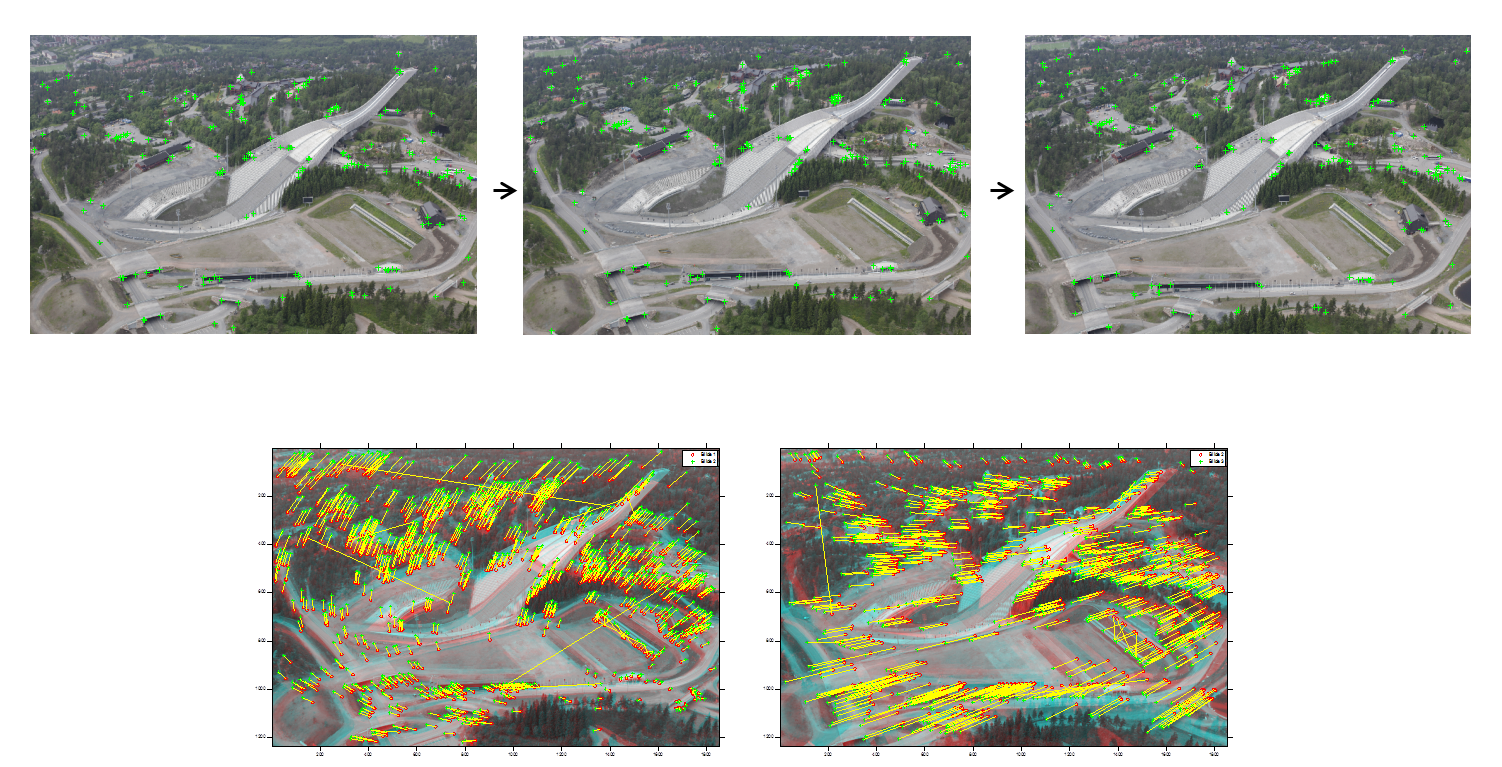
\includegraphics[width=\columnwidth]{figures/keypoint_matches.png}
    \caption{
    Tracking the scene in a sequence of images.
    In the top row, we see an example of how we can repeatedly detect corresponding points in the scene by extracting keypoint features. 
    By computing local descriptors around these points, we can search for putative point matches between the images, such as shown in the bottom row. 
    Outliers can be removed by only keeping matches that fit with the same type of motion hypothesis.
    }
    \label{fig:keypoint-matches}
\end{figure}
\begin{figure}[htb]
    \centering
    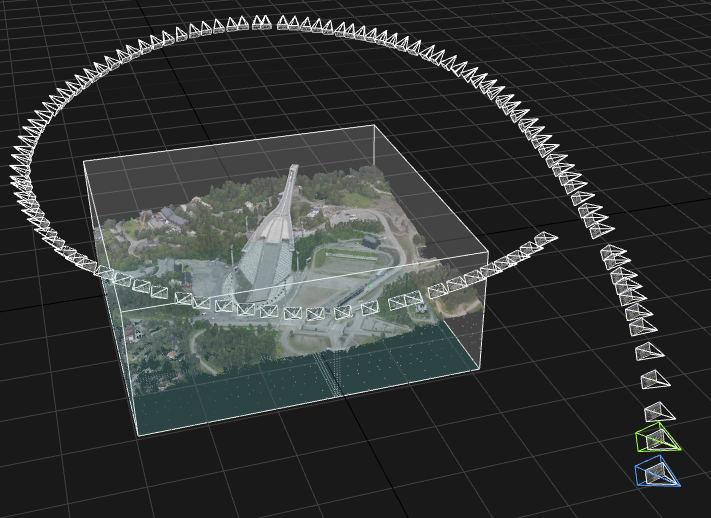
\includegraphics[width=0.75\columnwidth]{figures/holmenkollen-3d.png}
    \caption{An example of estimating motion and a 3D map from a sequence of images.}
    \label{fig:sfm}
\end{figure}

The map can be used to support tasks such as planning robot motion through rough terrain or avoiding obstacles.
It also allows us to limit the error in the motion estimation by serving as a reference for navigation.
By recognising revisited areas and correcting for drift through \emph{loop-closure} constraints, the robot can ``reset'' its localisation error and recover the true topology of the environment, as illustrated in Figure~\ref{fig:topology}.
This approach to navigation is often called \emph{Visual Simultaneous Localisation and Mapping (VSLAM)}.
Approaches that reduce computations and complexity by estimating maps locally without loop-closures are often called \emph{Visual Odometry (VO)} systems, and can be considered as reduced VSLAM systems, with the place recognition module disabled.
Such approaches reduce drift locally, but are unable to correct for drift in the long-term, and will not recover the global topology of the scene.
\begin{figure}[htb]
    \centering
    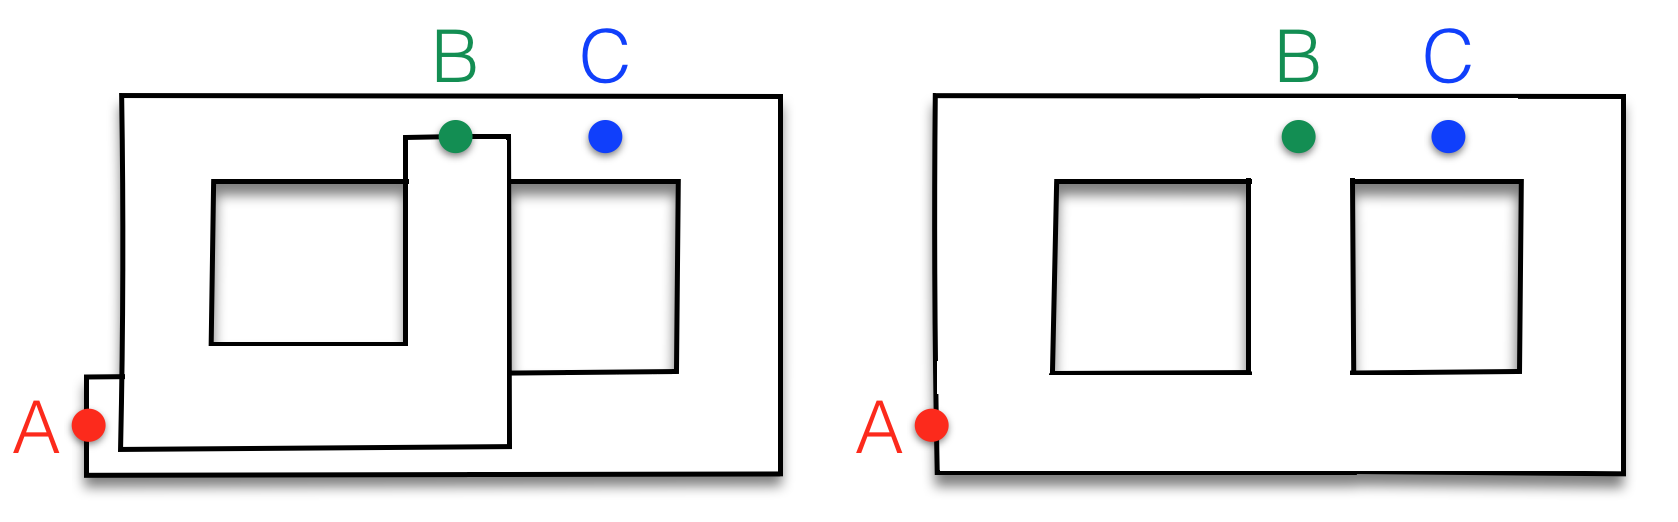
\includegraphics[width=0.75\columnwidth]{figures/topology.png}
    \caption{
    Left: Map built from odometry.
    Points that are close in reality (e.g. B and C) may be arbitrarily far away in the local map.
    Right: By leveraging loop-closures, VSLAM can recover the true topology of the environment, and discover ``shortcuts'' in the map.
    (Image source: \cite{Cadena2016})
    }
    \label{fig:topology}
\end{figure}

\begin{figure}[htb]
    \centering
    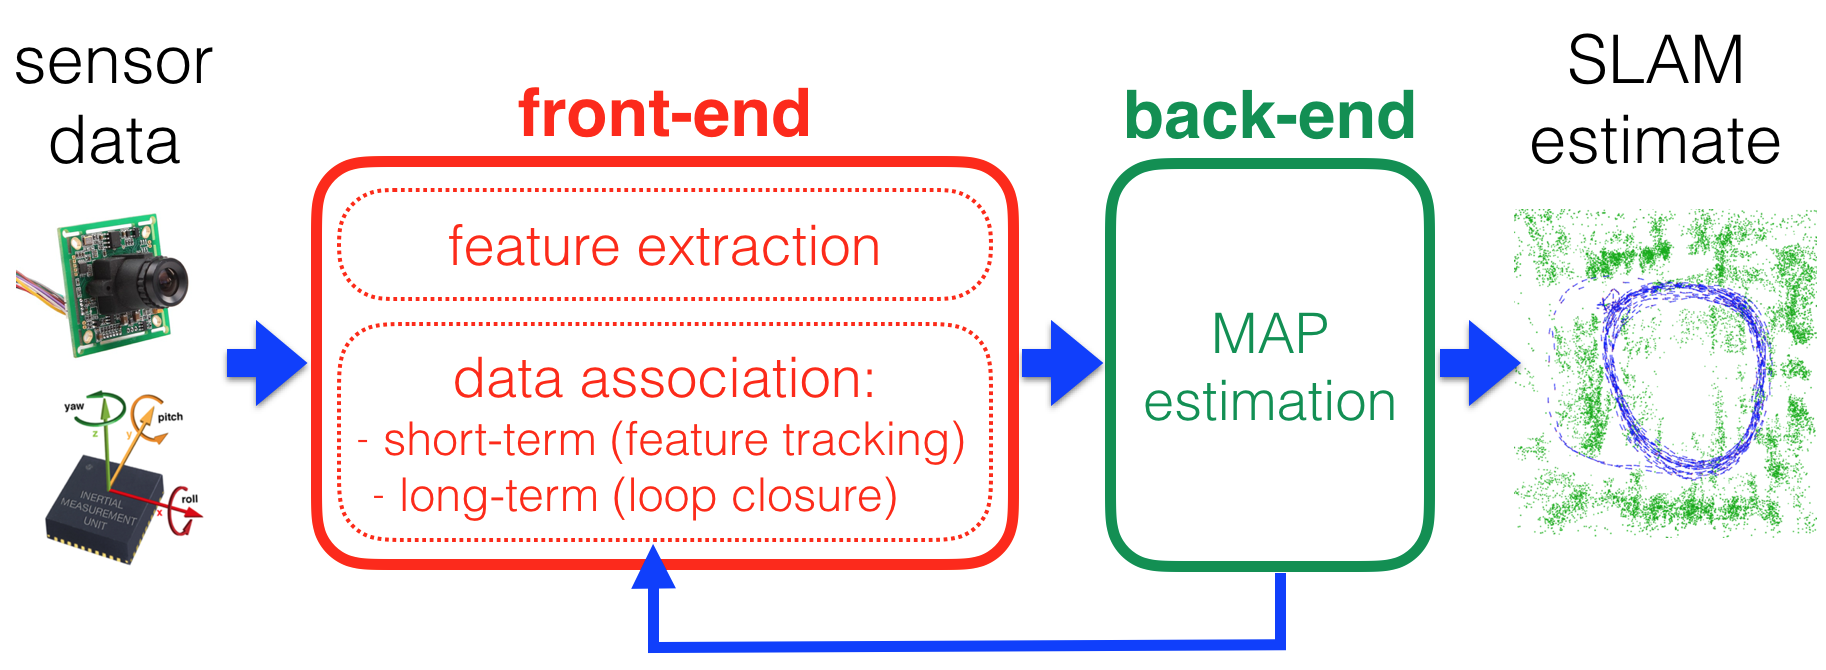
\includegraphics[width=0.75\columnwidth]{figures/frontBack.png}
    \caption{
    Front end and back end in a typical VSLAM system.
    (Image source: \cite{Cadena2016})
    }
    \label{fig:front-and-backend}
\end{figure}
It is customary to separate a SLAM system into two main components: the \emph{front end} and the \emph{back end} \cite{Cadena2016} (Figure~\ref{fig:front-and-backend}).
The front end extracts relevant data from raw sensor measurements, and performs data associations between the measurements and the map.
The back end performs estimation and inference on data from the front end.
Notice that the back end may also incorporate measurements from other types of sensors, such as \emph{inertial measurements units (IMUs)}.
We will here focus on the back end in VSLAM systems.

We may formulate the problem of estimating both motion and structure from noisy sensor measurements by using a Bayesian probabilistic model.
Assume that we want to estimate the unknown set of state variables $X$ that includes both the motion of the camera and the structure of the scene.
Also assume that we are given a set of sensor measurements $Z$ that depend upon the true state of $X$.
The most often used estimator for $X$ is the \emph{maximum a posteriori} (MAP) estimate, which maximises the posterior density $p(X | Z)$ of the states $X$ given the measurements $Z$.
By applying Bayes' law, we get
\begin{align*}
    X^\text{MAP} &= \argmax_X p(X | Z)\\[1em]
    &= \argmax_X \frac{p(Z | X) p(X)}{p(Z)}\\[1em]
    &= \argmax_X l(X;Z) p(X),
\end{align*}
where $l(X;Z) \propto p(Z | X)$ is the likelihood of the states $X$ given the measurements $Z$, defined as any function proportional to $p(Z | X)$.
This can be seen as a form of sensor model, that allows us to evaluate how well the measurements fit with our current hypothesis for the states $X$.
The density $p(X)$ is the prior density over the states, which allows us to evaluate how well our current hypothesis fits with any prior knowledge about $X$.

This handbook is meant to provide a terse, but thorough, introduction to the fundamentals behind how such problems may be expressed and solved.
We will start by covering how we can describe states and sensor models using 3D geometry and Lie theory.
This includes a framework for expressing derivatives of vectors, orientations and poses, and representing uncertainty in such variables.
We will then see how nonlinear least squares can be applied to find the MAP estimate for states, given noisy measurements and corresponding measurement prediction models.
Finally we will cover how this can be applied in estimating pose and structure from images.

Hopefully, this handbook will be useful background when studying Visual odometry and Visual SLAM systems.

%\chapter{Image formation}
Se også Ma.
Kan også droppes, vent med til slutt.
Geometry next chapter.

\begin{itemize}
    \item Photometry, is..., photometric error
    \item Also representation?
    \item Exposure, rolling shutter, 
    \item Noise characteristics, photon noise
    \item Also thermal
    \item Vignetting
    \item Mono vs Bayer, why mono...
    \item Gain, white balance, ...
    \item Model: Photon -> intensity
\end{itemize}

\chapter{3D geometry} \label{ch:3d-geometry}
We will in this chapter describe how we can relate different objects in 3D by defining local coordinate frames and transformations between them.
This will let us express the orientation and pose of objects relative to each other, which we can use to transform points between coordinate frames.
We will also introduce notation that makes the direction of these transformations explicit and easy to deduce.


\section{Points and coordinate frames} \label{sec:points-coordinate-frames}
\begin{figure}[htb]
    \centering
    \tdplotsetmaincoords{60}{110}
\begin{tikzpicture}[scale=2, tdplot_main_coords]
  \coordinate (O) at (0,0,0);
  \coordinate (P) at (0,4,2);
  
  \draw[thick, color=red, ->] (O) -- (1,0,0);
  \draw[thick, color=red, ->] (O) -- (0,1,0);
  \draw[thick, color=red, ->] (O) -- (0,0,1);
  \node[anchor=north, color=red] (Fa) at (0,0.1,-0.1) {$\cF_a \;$};
  
  \path (P) node[circle, fill, inner sep=1]{};
  \draw[-stealth, color=red] (O) -- (P)  node [midway, above] {$\vecx^a$};
  \node[anchor=west] at (P) {$X$};
\end{tikzpicture}

    \caption{A point $X$ represented by a vector $\vecx^a$ in the coordinate frame $\cF_a$.}
    \label{fig:coordinate_frame}
\end{figure}
A point in space may be described by a \emph{coordinate vector}, as shown in Figure \ref{fig:coordinate_frame}.
In this example, the point $X$ is described by the vector $\vecx^a \in \bbR^3$, which represents the displacement of the point in Euclidean space with respect to the \emph{coordinate frame} $\cF_a$.
A \emph{Cartesian coordinate frame} defines a set of orthogonal axes which intersect at a point called the origin.

An alternative to Cartesian coordinates in Euclidean space is to describe points using \emph{homogeneous coordinates} in projective space.
A homogeneous coordinate vector in projective space is given by $\tilde{\vecx} = [\tilde{x}, \tilde{y}, \tilde{z}, \tilde{w}]\trans \in \bbP^3$, where $\tilde{\vecx} = \lambda \tilde{\vecx}$ for all non-zero scalars $\lambda$.

Given a Cartesian coordinate vector $\vecx = [x, y, z]\trans \in \bbR^3$, we can represent the same point as the homogeneous coordinate vector $\tilde{\vecx} = \lambda[x, y, z, 1]\trans$.
This means that we can construct a homogeneous vector from a Cartesian vector with the mapping
\begin{equation} \label{eq:cart-to-homo}
  \vecx = 
  \begin{bmatrix}
  x\\
  y\\
  z
  \end{bmatrix}
  \in \bbR^3
  \quad \mapsto \quad
  \tilde{\vecx} = \breve{\vecx} =
  \begin{bmatrix}
  x\\
  y\\
  z\\
  1
  \end{bmatrix}
  \in \bbP^3,
\end{equation}
where we use the notation $\breve{\vecx}$ for the \emph{normalised} homogeneous coordinate $\breve{\vecx} = \begin{bsmallmatrix}\vecx\\ 1\end{bsmallmatrix}$, according to \emph{Euclidean normalisation}.
We can map a homogeneous vector back into a Cartesian vector with
\begin{equation} \label{eq:homo-to-cart}
  \tilde{\vecx} =
  \begin{bmatrix}
  \tilde{x}\\
  \tilde{y}\\
  \tilde{z}\\
  \tilde{w}
  \end{bmatrix}
  \in \bbP^3
  \quad \mapsto \quad
  \vecx = 
  \begin{bmatrix}
  \tilde{x} / \tilde{w}\\
  \tilde{y} / \tilde{w}\\
  \tilde{z} / \tilde{w}
  \end{bmatrix}
  \in \bbR^3.
\end{equation}
Homogeneous vectors with $\tilde{w} = 0$ have no representation in $\bbR^3$, and correspond to the direction to points infinitely far away from the origin.
As we will see later, homogeneous coordinates are a convenient representation when describing transformations and camera projections of points and directions.
See Hartley and Zisserman \cite{Hartley2004MultipleVision} for a detailed description of projective geometry for computer vision.

\begin{figure}[htb]
    \centering
    \tdplotsetmaincoords{60}{110}
\begin{tikzpicture}[scale=2, tdplot_main_coords]
  \coordinate (O) at (0,0,0);
  \coordinate (P) at (0,4,2);
  
  \draw[thick, color=red, ->] (O) -- (1,0,0);
  \draw[thick, color=red, ->] (O) -- (0,1,0);
  \draw[thick, color=red, ->] (O) -- (0,0,1);
  \node[anchor=north, color=red] (Fa) at (0,0.1,-0.1) {$\cF_a \;$};
  
  \path (P) node[circle, fill, inner sep=1]{};
  \node[anchor=west] at (P) {$X$};
  
  \draw[-stealth, color=red] (O) -- (P)  node [midway, above] {$\vecx^a$};
  
  \coordinate (W) at (3, 3, 1);
  \tdplotsetrotatedcoords{30}{0}{0};
  \tdplotsetrotatedcoordsorigin{(W)};
  
  \draw[thick, color=green!50!black, tdplot_rotated_coords,->] (0,0,0) -- (1,0,0);
  \draw[thick, color=green!50!black, tdplot_rotated_coords,->] (0,0,0) -- (0,1,0);
  \draw[thick, color=green!50!black, tdplot_rotated_coords,->] (0,0,0) -- (0,0,1);
  \node[anchor=north east, color=green!50!black, tdplot_rotated_coords] (Fb) at (0,0,0) {$\cF_b \;$};
  
  \draw[-stealth, tdplot_rotated_coords, color=green!50!black] (0,0,0) -- (P)  node [midway, above] {$\vecx^b$};
  
  \draw[-stealth, densely dotted] (Fa)  to [bend right=60]  node [midway, below] {$\matT_{ab}$} (Fb);
  
  
\end{tikzpicture}

    \caption{A point $X$ represented by a vector $\vecx^a$ in the coordinate frame $\cF_a$, and a corresponding vector $\vecx^b$ in the coordinate frame $\cF_b$.
    The pose $\matT_{ab}$ describes the position and orientation of $\cF_b$ relative to $\cF_a$.}
    \label{fig:more_frames}
\end{figure}
It is sometimes necessary to describe the same point relative to several coordinate frames.
We might for example want to relate a point given in a world frame to the local coordinate frame of a camera.
The relationship between the Cartesian coordinate frames in Figure~\ref{fig:more_frames} can be described by the \emph{position} and \emph{orientation} of $\cF_b$ relative to $\cF_a$.
This is also called the \emph{pose} of $\cF_b$ relative to $\cF_a$, and can be expressed as a transformation $\matT_{ab}$ that lets us map the point's coordinates $\vecx^b$ in $\cF_b$ to coordinates $\vecx^a$ in $\cF_a$.

We will in the following sections see how we can represent and apply such transformations between coordinate frames.


\section{Representing orientation} \label{sec:orientation}
\begin{figure}[htb]
    \centering
    \tdplotsetmaincoords{60}{110}
\begin{tikzpicture}[scale=2, tdplot_main_coords]
  \coordinate (O) at (0,0,0);
  
  \draw[thick, color=red,->] (O) -- (1,0,0) node[anchor=north east]{$\veca_1$};
  \draw[thick, color=red,->] (O) -- (0,1,0) node[anchor=south west]{$\veca_2$};
  \draw[thick, color=red,->] (O) -- (0,0,1) node[anchor=south east]{$\veca_3$};
  \node[anchor=east, color=red] (Fa) at (O) {$\cF_a \;$};
  
  \tdplotsetrotatedcoords{45}{20}{20};
  
  \draw[thick, color=green!50!black, tdplot_rotated_coords,->] (0,0,0) -- (1,0,0) node[anchor=north]{$\vecb_1$};
  \draw[thick, color=green!50!black, tdplot_rotated_coords,->] (0,0,0) -- (0,1,0) node[anchor=west]{$\vecb_2$};
  \draw[thick, color=green!50!black, tdplot_rotated_coords,->] (0,0,0) -- (0,0,1) node[anchor=south west]{$\vecb_3$};
  \node[anchor=north, color=green!50!black] (Fb) at (0.2,0.2,0) {$\cF_b \;$};
  
  \draw[-stealth, densely dotted] (Fa)  to [bend right=60]  node [near start, left] {$\matR_{ab}$} (Fb);
  
\end{tikzpicture}

    \caption{Two coordinate frames $\cF_a$ and $\cF_b$ with the same origin. The orientation of $\cF_b$ relative to $\cF_a$ is described by the rotation matrix $\matR_{ab}.$}
    \label{fig:rotated_frames}
\end{figure}

We can describe the orientation of coordinate frame $\cF_b$ relative to $\cF_a$ by how we should rotate $\cF_a$ in order to align with $\cF_b$.
This rotation has 3 degrees of freedom (DOF), and can be represented by the orthogonal rotation matrix
\begin{equation}
  \matR_{ab} = 
  \begin{bmatrix}
  r_{11} & r_{12} & r_{13}\\
  r_{21} & r_{22} & r_{23}\\
  r_{31} & r_{32} & r_{33}
  \end{bmatrix}
  \in \SO(3).
\end{equation}
Rotation matrices belong to the $\SO(3)$ Lie group (special orthogonal group of dimension 3), which we will cover in more detail in Section \ref{sec:SO3_group}.

Let the coordinate frame $\cF_a$ be defined by the orthonormal basis vectors $\{\veca_1, \veca_2, \veca_3\}$, and the frame $\cF_b$ be defined by the orthonormal basis vectors $\{\vecb_1, \vecb_2, \vecb_3\}$, as illustrated in Figure \ref{fig:rotated_frames}.
The columns of the rotation matrix representing the orientation of $\cF_b$ relative to $\cF_a$ correspond to the basis vectors of $\cF_b$ expressed in frame $\cF_a$
\begin{equation} \label{eq:rot_basis}
  \matR_{ab} = 
  \begin{bmatrix}
    \vecb^a_1 & \vecb^a_2 & \vecb^a_3
  \end{bmatrix}.
\end{equation}
When the coordinate frames have the same origin, this lets us use the orientation of $\cF_b$ relative to $\cF_a$ to transform points $\vecx^b$ given in frame $\cF_b$ to points $\vecx^a$ given in frame $\cF_a$ by
\begin{equation}
  \vecx^a = \matR_{ab} \vecx^b.
\end{equation}

\begin{figure}[htb]
    \centering
    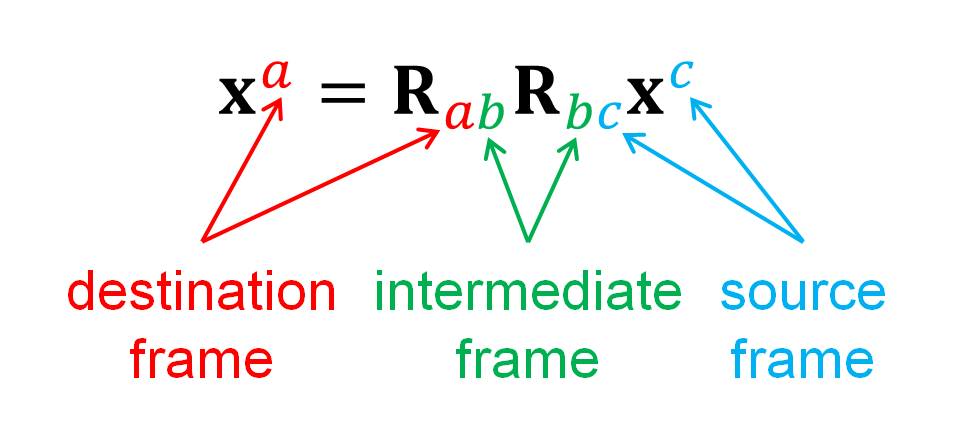
\includegraphics[width=0.5\columnwidth]{figures/coordinate_frame_notation.png}
    \caption{The coordinate frame notation helps us combine transformations in the correct order.}
    \label{fig:coordinate-frame-notation}
\end{figure}

We can also compose relative orientations with matrix multiplication
\begin{equation}
  \matR_{ac} = \matR_{ab} \matR_{bc}.
\end{equation}
The inverse orientation is given by the inverse rotation matrix, and since rotation matrices are orthogonal, we have
\begin{equation}
  \matR_{ba} = \matR_{ab}^{-1} = \matR_{ab}\trans.
\end{equation}
Notice in Figure \ref{fig:coordinate-frame-notation} how the subscript and superscript notation for coordinate frames aligns, and helps us combine transformations in the correct order.

\begin{example}[frametitle=Transforming detections between sensors]
{
  \centering
  \tdplotsetmaincoords{10}{45}
\begin{tikzpicture}[scale=2, tdplot_main_coords]
  \coordinate (O) at (0,0,0);
  \coordinate (P) at (1.75,2.25,0);
  
  \draw[thick, color=green!50!black,->] (O) -- (1,0,0);
  \draw[thick, color=green!50!black,->] (O) -- (0,1,0);
  \draw[thick, color=green!50!black,->] (O) -- (0,0,1);
  \node[anchor=east, color=green!50!black, tdplot_screen_coords] (Fb) at (-0.3, 0, 0) {$\cF_b \;$};
  
  \tdplotsetrotatedcoords{-30}{-10}{0};
  \draw[thick, color=blue, tdplot_rotated_coords,->] (0,0,0) -- (1,0,0);
  \draw[thick, color=blue, tdplot_rotated_coords,->] (0,0,0) -- (0,1,0);
  \draw[thick, color=blue, tdplot_rotated_coords,->] (0,0,0) -- (0,0,1);
  \node[anchor=east, color=blue, tdplot_screen_coords] (Fc) at (-0.3, -0.75) {$\cF_c \;$};
  \draw[-stealth, tdplot_rotated_coords, color=blue] (0,0,0) -- (P)  node [near end, above] {$\vecx^c$};
  \path (P) node[circle, fill, inner sep=1]{};
  \node[anchor=west] at (P) {$X$};
  
  \tdplotsetrotatedcoords{30}{10}{10};
  \draw[thick, color=red, tdplot_rotated_coords,->] (0,0,0) -- (1,0,0);
  \draw[thick, color=red, tdplot_rotated_coords,->] (0,0,0) -- (0,1,0);
  \draw[thick, color=red, tdplot_rotated_coords,->] (0,0,0) -- (0,0,1);
  \node[anchor=east, color=red, tdplot_screen_coords] (Fa) at (-0.3, 0.75) {$\cF_a \;$};
  
  \draw[-stealth, densely dotted] (Fb)  to [bend left=60]  node [midway, left] {$\matR_{ba}$} (Fa);
  \draw[-stealth, densely dotted] (Fb)  to [bend right=60]  node [midway, left] {$\matR_{bc}$} (Fc);
  
  
\end{tikzpicture}

  \captionsetup{type=figure}
  \captionof{figure}{Three differently oriented sensors.}
  \label{fig:orientation_example}
  \par
}

Assume that we have three coordinate frames $\cF_a$, $\cF_b$ and $\cF_c$ at the same origin, as shown in Figure~\ref{fig:orientation_example}.
These correspond to three co-located, but differently oriented sensors.
The sensor system has been calibrated with regards to sensor $b$, so we are given $\matR_{ba}$ and $\matR_{bc}$.
When the sensor $c$ detects a point $\vecx^c$ represented in frame $\cF_c$, what is the corresponding position in the coordinate frame of sensor $a$?

We can represent the relative orientation between $\cF_c$ and $\cF_a$ using the calibrated orientations by
\begin{equation}
  \matR_{ac} = \matR_{ab} \matR_{bc} = \matR_{ba}\trans \matR_{bc}.
\end{equation}
This lets us compute the point represented in $\cF_a$ as
\begin{equation}
  \vecx^a = \matR_{ac} \vecx^c = \matR_{ba}\trans \matR_{bc} \vecx^c.
\end{equation}
\end{example}

Since $\matR_{ba} = \matR_{ab}\trans$, we see from \eqref{eq:rot_basis} that the rows of $\matR_{ba}$ are given by the basis vectors of $\cF_a$ expressed in frame $\cF_b$
\begin{equation} \label{eq:rot_basis_rows}
  \matR_{ab} = 
  \begin{bmatrix}
    {\veca^b_1}\trans\\
    {\veca^b_2}\trans\\
    {\veca^b_3}\trans
  \end{bmatrix}.
\end{equation}
This is sometimes useful when assessing how coordinate systems relate to each other.

\begin{example}[frametitle=Rotation matrix from basis vector perturbations]
{
  \centering
  \tdplotsetmaincoords{-120}{70}
\begin{tikzpicture}[scale=2, tdplot_main_coords]
  \coordinate (O) at (0,0,0);
  
  \draw[thick, color=red,->] (O) -- (1,0,0) node[anchor=south east]{$\veca_1$};
  \draw[thick, color=red,->] (O) -- (0,1,0) node[anchor=south west]{$\veca_2$};
  \draw[thick, color=red,->] (O) -- (0,0,1) node[anchor=north west]{$\veca_3$};
  \node[anchor=east, color=red] (Fa) at (0.2, -0.1, 0) {$\cF_a \;$};
  
  \tdplotsetrotatedcoords{0}{90}{90};
  
  \draw[thick, dashed, color=green!50!black, tdplot_rotated_coords,->] (0,0,0) -- (1,0,0) node[anchor=north]{$\vecb_1$};
  \draw[thick, dashed, color=green!50!black, tdplot_rotated_coords,->] (0,0,0) -- (0,1,0) node[anchor=east]{$\vecb_2$};
  \draw[thick, dashed, color=green!50!black, tdplot_rotated_coords,->] (0,0,0) -- (0,0,1) node[anchor=west]{$\vecb_3$};
  \node[anchor=north, color=green!50!black] (Fb) at (0,0.2,0.1) {$\cF_b \;$};
  
  \draw[-stealth, densely dotted] (Fa)  to [bend right=60]  node [midway, left] {$\matR_{ab}$} (Fb);
  
\end{tikzpicture}

  \captionsetup{type=figure}
  \captionof{figure}{Two coordinate frames with their corresponding basis vectors.}
  \label{fig:perturbed_basis_example}
  \par
}

As shown in Figure \ref{fig:perturbed_basis_example}, we have a coordinate frame $\cF_a$, where the $x$-axis points forwards, the $y$-axis points right and the $z$-axis points down.
We also have a coordinate frame $\cF_b$ where the $z$-axis points forwards and the $x$-axis points right.
What is the orientation $\matR_{ab}$ of $\cF_b$ relative to $\cF_a$?

From \eqref{eq:rot_basis} we know that the columns of $\matR_{ab}$ correspond to the basis vectors of $\cF_b$ relative to $\cF_a$.
Since $\vecb^a_1 = \veca_2$, $\vecb^a_2 = \veca_3$ and $\vecb^a_3 = \veca_1$, we get
\begin{equation} \label{eq:rot_basis_example}
  \matR_{ab} = 
  \begin{bmatrix}
    \veca_2 & \veca_3 & \veca_1
  \end{bmatrix}
  =
  \begin{bmatrix}
    0 & 0 & 1\\
    1 & 0 & 0\\
    0 & 1 & 0
  \end{bmatrix}.
\end{equation}

With \eqref{eq:rot_basis_rows}, we can now also confirm that the rows of \eqref{eq:rot_basis_example} correspond to the basis vectors of $\cF_a$ relative to $\cF_b$.
\end{example}

Rotations about the basis vectors are called \emph{principal rotations}.
The rotation matrices for a rotation $\theta$ about the $x$-, $y$- and $z$-axes are given by
\begin{align}
  \matR_x(\theta) &= 
  \begin{bmatrix}
    1 & 0 & 0\\
    0 & \cos \theta & -\sin \theta\\
    0 & \sin \theta & \cos \theta
  \end{bmatrix}\\[1em]
  %
  \matR_y(\theta) &= 
  \begin{bmatrix}
    \cos \theta & 0 & \sin \theta\\
    0 & 1 & 0\\
    -\sin \theta & 0 & \cos \theta
  \end{bmatrix}\\[1em]
  %
  \matR_z(\theta) &= 
  \begin{bmatrix}
    \cos \theta & -\sin \theta & 0\\
    \sin \theta & \cos \theta & 0\\
    0 & 0 & 1
  \end{bmatrix}.
\end{align}
Any orientation can be represented by a sequence of three principal rotations, where no two successive rotations are about the same axis.
This lets us specify an orientation as a set of three angles $(\theta_1, \theta_2, \theta_3)$ and a corresponding sequence of principal rotations, which is often referred to as the Euler angle representation.

\begin{example}[frametitle={Orientation represented as roll, pitch and yaw}]
{
  \centering
  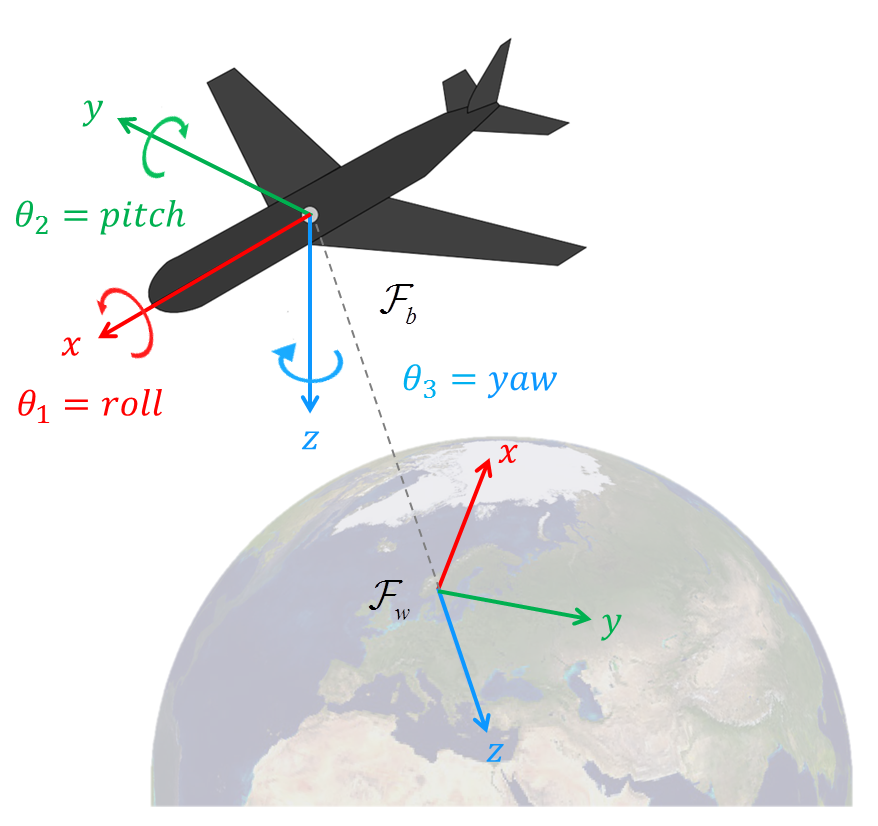
\includegraphics[width=0.5\columnwidth]{figures/roll-pitch-yaw_NED.png}
  \captionsetup{type=figure}
  \captionof{figure}{The orientation of the body frame $\cF_b$ (front, right, down) relative to the world frame $\cF_w$ (north, east, down) is represented with roll-, pitch- and yaw-angles about the body axes.}
  \label{fig:roll-pitch-yaw_example}
  \par
}

We have an aircraft with body coordinate frame $\cF_b$, where the $x$-axis points forward, the $y$-axis points right and the $z$-axis points down.
The world coordinate frame $\cF_w$ is given as a NED frame, where the $x$-axis points north, the $y$-axis points east and the $z$-axis points down.
The roll-, pitch- and yaw-angles around the principal axes of $\cF_b$ are given as $(\theta_1, \theta_2, \theta_3)$, as shown in Figure \ref{fig:roll-pitch-yaw_example}.

We can compute the rotation matrix corresponding to the orientation of $\cF_b$ relative to $\cF_w$ with the roll-pitch-yaw sequence of principal rotations
\begin{equation}
  \matR_{wb} = \matR_z(\theta_3) \matR_y(\theta_2) \matR_x(\theta_1).
\end{equation}
\end{example}

It is also possible to describe any orientation as a rotation about a given axis.
This is called the \emph{angle-axis} representation, and can be expressed as
\begin{equation}
  \vectheta = \theta \vecu,
\end{equation}
where $\theta$ is the angle of rotation and $\vecu$ is the unit-length axis of rotation.
The corresponding rotation matrix is given by Rodrigues' rotation formula
\begin{equation} \label{eq:rot-from-axis-angle}
  \matR(\vectheta) = \matI + \sin \theta [\vecu]_\times + (1 - \cos \theta) [\vecu]^2_\times, 
\end{equation}
where $[\vecu]_\times$ is the skew-symmetric matrix\footnotemark
\begin{equation}
  [\vecu]_\times =
  \begin{bmatrix}
    u_1\\
    u_2\\
    u_3
  \end{bmatrix}_\times \triangleq
  \begin{bmatrix}
    0 & -u_3 & u_2\\
    u_3 & 0 & -u_1\\
    -u_2 & u_1 & 0
  \end{bmatrix}.
\end{equation}
When the angle $\theta$ is small, the corresponding rotation matrix can be approximated with the matrix
\begin{equation} \label{eq:infinitesimal-rotaton}
  \matR(\vectheta) \approx \matI + [\vectheta]_\times.
\end{equation}
This is sometimes called an \emph{infinitesimal rotation}.
\footnotetext{The cross product between two vectors can also be represented as a matrix multiplication using this skew-symmetric matrix: $\veca \times \vecb = [\veca]_\times \vecb$. This explains the common $[\cdot]_\times$ notation.}

Another similar and very popular representation for rotation is the \emph{unit quaternion}, which is covered in detail in e.g. \cite{barfoot2017state}.

The orthogonal rotation matrix has 9 elements that parameterise the 3 DOF rotation.
The Euler angle and angle-axis representations are both minimal representations, in that they both can be represented by 3 parameters, but they suffer from singularities.
In fact, there is no perfect representation that is minimal and also free of singularities.
This is because 3D rotations lie on a 3D manifold embedded in a higher dimensional space.
We will in Chapters~\ref{sec:Lie-theory},~\ref{ch:jacobians} and \ref{ch:uncertainty} see how we can describe perturbations, derivatives and probability distributions on this manifold.

\section{Representing pose}
\begin{figure}[htb]
    \centering
    \tdplotsetmaincoords{60}{110}
\begin{tikzpicture}[scale=2, tdplot_main_coords]
  \coordinate (O) at (0,0,0);
  
  \draw[thick, color=red, ->] (O) -- (1,0,0);
  \draw[thick, color=red, ->] (O) -- (0,1,0);
  \draw[thick, color=red, ->] (O) -- (0,0,1);
  \node[anchor=north, color=red] (Fa) at (0,0.1,-0.1) {$\cF_a \;$};
  
  \coordinate (W) at (3, 3, 1);
  \tdplotsetrotatedcoords{30}{0}{0};
  \tdplotsetrotatedcoordsorigin{(W)};
  
  \draw[thick, color=green!50!black, tdplot_rotated_coords,->] (0,0,0) -- (1,0,0);
  \draw[thick, color=green!50!black, tdplot_rotated_coords,->] (0,0,0) -- (0,1,0);
  \draw[thick, color=green!50!black, tdplot_rotated_coords,->] (0,0,0) -- (0,0,1);
  \node[anchor=north east, color=green!50!black, tdplot_rotated_coords] (Fb) at (0,0,0) {$\cF_b \;$};
  
  \draw[-stealth, densely dotted] (Fa)  to [bend right=60]  node [midway, below] {$\matR_{ab}$} (Fb);
  \draw[-stealth, color=red] (O) -- (W)  node [near end, above] {$\vect^a_{ab}$};
  
\end{tikzpicture}

    \caption{Two coordinate frames $\cF_a$ and $\cF_b$ with different position and orientation. The pose of $\cF_b$ relative to $\cF_a$ is described by the orientation $\matR_{ab}$ and the translation $\vect^a_{ab}$ between the frame origins.}
    \label{fig:pose-illustration}
\end{figure}

When coordinate frames do not share a common origin, we also need to take the relative position between frames into account.
The \emph{pose} of $\cF_b$ relative to $\cF_a$ describes how $\cF_a$ should be rotated \emph{and} translated in order to coincide with $\cF_b$.
This can be represented with the homogeneous transformation matrix
\begin{equation}
  \matT_{ab} = 
  \begin{bmatrix}
  \matR_{ab} & \vect^a_{ab}\\[0.3em]
  \matr{0}\trans & 1
  \end{bmatrix}
  \in \SE(3),
\end{equation}
where $\matR_{ab} \in \SO(3)$ represents the orientation of $\cF_b$ relative to $\cF_a$, and $\vect^a_{ab} \in \bbR^3$ is a translation vector given in the coordinate frame of $\cF_a$.
This vector represents the position of $\cF_b$ relative to $\cF_a$, as shown in Figure \ref{fig:pose-illustration}.
The $4 \times 4$ pose matrices are known as \emph{3D Euclidean} or \emph{3D rigid body} transformations, and belong to the $\SE(3)$ Lie group (special Euclidean group of dimension 3), which we will cover in more detail in Section \ref{sec:SE3_group}.

The fact that $\matT$ is a homogeneous transformation matrix means that we can express the Euclidean transformation linearly using homogeneous vectors.
Given a point $\vecx^b$ represented in $\cF_b$ and the pose $\matT_{ab}$ of $\cF_b$ relative to $\cF_a$, we can convert to the homogeneous representation $\tilde{\vecx}^b$ using \eqref{eq:cart-to-homo}, and transform the point to coordinates given in frame $\cF_a$ by
\begin{equation} \label{eq:homo-pose-transf}
  \tilde{\vecx}^a = \matT_{ab} \tilde{\vecx}^b.
\end{equation}
We get the Cartesian coordinate $\vecx^a$ by normalising $\tilde{\vecx}^a$ according to \eqref{eq:homo-to-cart}.

The transformation in \eqref{eq:homo-pose-transf} corresponds to rotating $\vecx^b$ into frame $\cF_a$, and translating according to the position of $\cF_b$ relative to $\cF_a$.
We can therefore express the transformation equivalently on Cartesian form as
\begin{equation}
  \vecx^a = \matR_{ab} \vecx^b + \vect^a_{ab}.
\end{equation}
%Although this form is less concise, we avoid the use of homogeneous coordinates, and can operate on the orientation $\matR$ and translation $\vect$ directly.
We will call this transformation the \emph{action} of the pose $\matT$ on the vector $\vecx$, and denote it as $\matT \cdot \vecx$, where
\begin{equation}
  \vecx^a = \matT_{ab} \cdot \vecx^b = \matR_{ab} \vecx^b + \vect^a_{ab}.
\end{equation}

As for rotations, we can compose relative poses with matrix multiplication.
This can also be expressed directly as operations on $\matR$ and $\vect$ by
\begin{equation}
  \matT_{ac} = \matT_{ab} \matT_{bc} =
  \begin{bmatrix}
    \matR_{ab} \matR_{bc} & \matR_{ab} \vect^b_{bc} + \vect^a_{ab}\\[0.3em]
    \matr{0}\trans & 1
  \end{bmatrix}
\end{equation}
The inverse pose is given by
\begin{equation}
  \matT_{ba} = \matT_{ab}^{-1} = 
  \begin{bmatrix}
    \matR_{ab}\trans  & -\matR_{ab}\trans \vect^a_{ab}\\[0.3em]
    \matr{0}\trans & 1
  \end{bmatrix}.
\end{equation}

Since all pose operations can be expressed as operations on the orientation and position directly, it is common to implement poses in practice as a pair $(\matR, \vect)$, rather than the full matrix $\matT$.
This avoids the use of homogeneous coordinates, and allows alternative representations for orientation, such as quaternions.
This dual representation lets us exploit the mathematical properties of $\matT$, while simultaneously reaping the benefits of the chosen implementation for orientation and pose operations.

\begin{example}[frametitle=Seeing a point in the world with a camera]
{
  \centering
  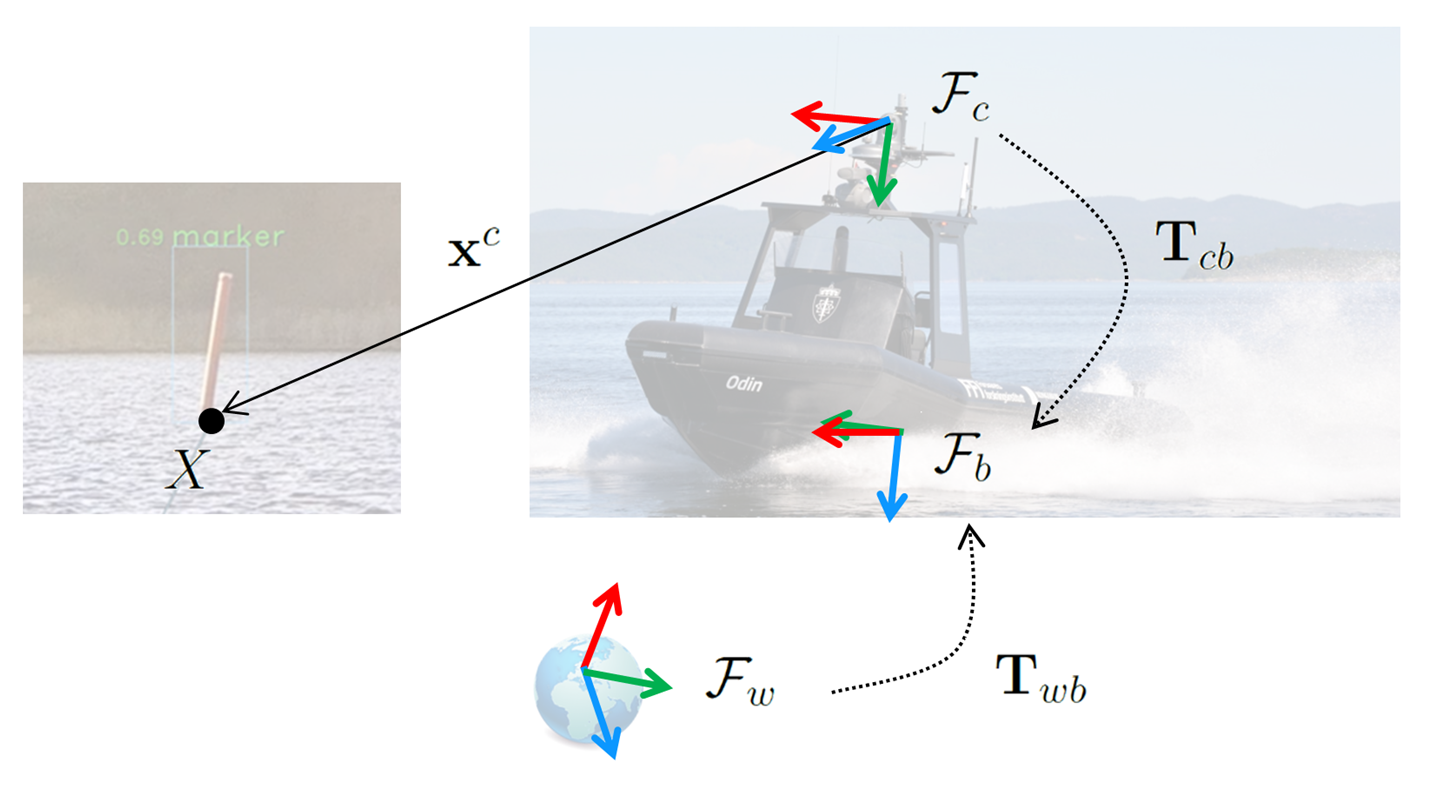
\includegraphics[width=0.75\columnwidth]{figures/odin_pose_example.png}
  \captionsetup{type=figure}
  \captionof{figure}{A camera observes a sea marker in the camera frame $\cF_c$. A navigation system estimates the pose of the boat relative to the world frame $\matT_{wb}$, and the pose of the boat relative to the camera $\matT_{cb}$ is known.}
  \label{fig:odin_pose_example}
  \par
}

An autonomous boat observes a sea marker in its camera frame $\cF_c$.
As illustrated in Figure~\ref{fig:odin_pose_example}, we are given the pose of the boat relative to the world frame $\matT_{wb}$, as well as the pose of the boat relative to the camera frame $\matT_{cb}$.
Where is the sea marker relative to the world frame $\cF_w$?

We can compute the pose of the camera relative to the world by
\begin{subequations}
\begin{align}
  \matT_{wc} &= \matT_{wb} \matT_{bc}\\
  &= \matT_{wb} \matT_{cb}^{-1}\\
  &=
  \begin{bmatrix}
    \matR_{wb} \matR_{cb}\trans  & -\matR_{wb} \matR_{cb}\trans \vect^c_{cb} + \vect^w_{wb}\\[0.3em]
    \matr{0}\trans & 1
  \end{bmatrix}.
\end{align}
\end{subequations}
The coordinate of the sea marker in the world frame is then
\begin{equation}
  \tilde{\vecx}^w = \matT_{wc} \tilde{\vecx}^c = \matT_{wb} \matT_{cb}^{-1} \tilde{\vecx}^c,
\end{equation}
or equivalently
\begin{subequations}
\begin{align}
  \vecx^w &= \matT_{wc} \cdot \vecx^c\\
  &= \matR_{wc} \vecx^c + \vect^w_{wc}\\
  &= \matR_{wb} \matR_{cb}\trans \vecx^c - \matR_{wb} \matR_{cb}\trans \vect^c_{cb} + \vect^w_{wb}.
\end{align}
\end{subequations}
\end{example}

\chapter{Camera geometry}
This chapter will introduce two important topics in camera geometry: The \emph{geometric camera model}, that describes the camera projection process, and the \emph{epipolar geometry}, that describes the geometry when seeing the same points from two different views.
Most of this chapter is based on the wonderful books by Hartley and Zisserman, and Ma et al. \cite{Hartley2004MultipleVision, Ma2004AnVision}.

\section{Geometric camera models}
In the general case, a geometric camera model is a  \emph{projection} $\pi: \bbR^3 \to \Omega$, which projects 3D points $\vecx^c \in \bbR^3$ in the camera frame $\cF_c$ onto pixels $\vecu \in \Omega$ in the image, so that
\begin{equation}
  \vecu = 
  \begin{bmatrix}
  u\\
  v
  \end{bmatrix}
  = \pi(\vecx^c).
\end{equation}
Here, $\Omega \subset \bbR^2,$ is the \emph{image domain} of all valid pixels.
The inverse of this function is the \emph{backprojection} $\pi^{-1}: \Omega \times \bbR^+ \to \bbR^3$, which maps pixels and a corresponding depth $z$ back to 3D points:
\begin{equation}
  \vecx^c =
  \begin{bmatrix}
  x^c\\
  y^c\\
  z^c
  \end{bmatrix}
  = \pi^{-1}(\vecu, z).
\end{equation}
We will in the following let $\vecu \in \bbR^2$, and assume that there is an implicit second step that ensures that $\vecu$ is a valid pixel $\in \Omega$.

When describing camera projections, it is often convenient to exploit the homogeneous point representation.
Equivalent to the homogeneous representation of 3D coordinates in Section~\ref{sec:points-coordinate-frames}, we can construct a homogeneous 2D vector from a 2D Cartesian vector with the mapping
\begin{equation} \label{eq:cart-to-homo-2d}
  \vecu = 
  \begin{bmatrix}
  u\\
  v
  \end{bmatrix}
  \in \bbR^2
  \quad \mapsto \quad
  \tilde{\vecu} = \breve{\vecu} =
  \begin{bmatrix}
  u\\
  v\\
  1
  \end{bmatrix}
  \in \bbP^2,
\end{equation}
and we can map a homogeneous vector back into a Cartesian vector with
\begin{equation} \label{eq:homo-to-cart-2d}
  \tilde{\vecu} =
  \begin{bmatrix}
  \tilde{u}\\
  \tilde{v}\\
  \tilde{w}
  \end{bmatrix}
  \in \bbP^2
  \quad \mapsto \quad
  \vecu = 
  \begin{bmatrix}
  \tilde{u} / \tilde{w}\\
  \tilde{v} / \tilde{w}
  \end{bmatrix}
  \in \bbR^2.
\end{equation}

\begin{figure}[htb]
    \centering
    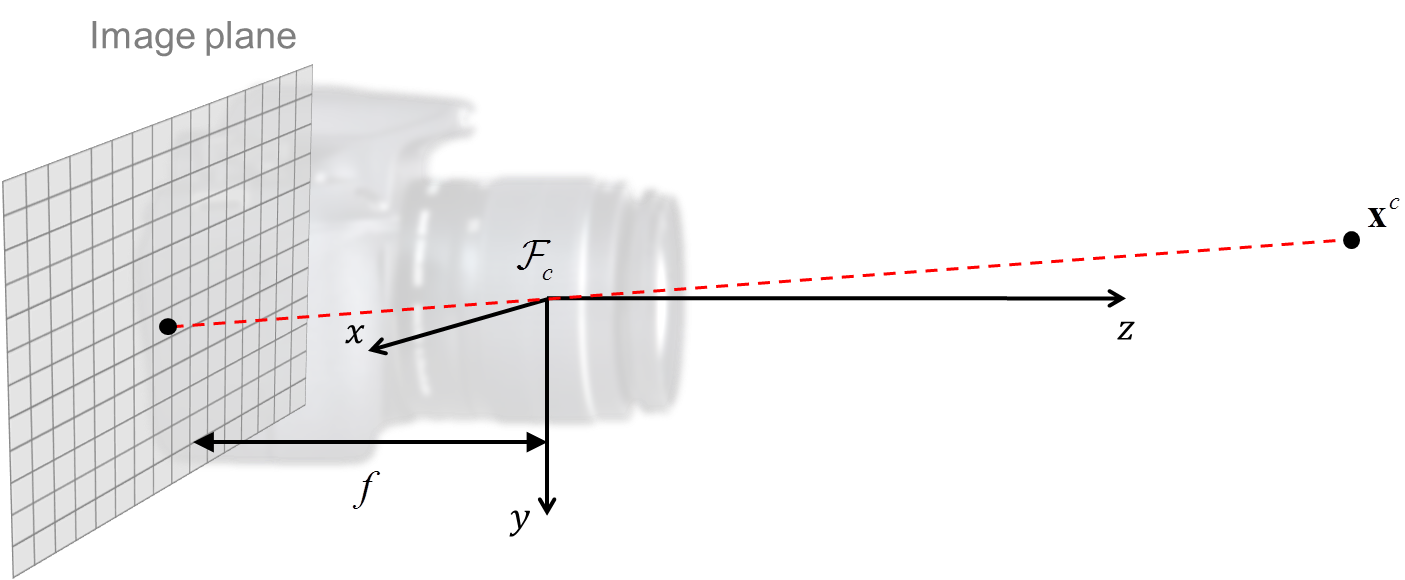
\includegraphics[height=5.5cm]{figures/perspective-camera-model-geometry.png}
    \caption{The imaging geometry in the perspective camera model.
    The camera is represented by the camera frame $\cF_c$.
    Points $\vecx^c$ in the camera frame are projected through the origin and onto the image plane at a distance $f$ behind the projective centre, where $f$ is the focal length.
    }
    \label{fig:perspective-camera-model-geometry}
\end{figure}
%
The most commonly used geometric camera model is the \emph{perspective camera model}\footnotemark.
As shown in Figure~\ref{fig:perspective-camera-model-geometry}, the camera is represented by a 3D coordinate frame $\cF_c$, with its origin at the camera's projective centre.
The $x$-axis is pointing right, the $y$-axis is pointing down, and the $z$-axis is pointing forwards along the \emph{optical axis} of the camera.
The imaging process is modelled as a central projection onto the image plane at $z = -f$, where $f$ is the \emph{focal length}.
\footnotetext{Sometimes also called the \emph{pinhole model}.}

Since the projection in Figure~\ref{fig:perspective-camera-model-geometry} results in images that are flipped upside down, it is more convenient to put the imaging plane in front of the projection centre using the \emph{frontal projection model}.
It is also convenient to define a \emph{normalised image plane} at $z = 1$, which represents an \emph{idealised camera} with focal length $1$, as illustrated in Figure~\ref{fig:perspective-camera-model_normalised}.
This lets us describe the imaging process at a fixed imaging plane, independently of the camera-specific focal length parameter $f$.

\begin{figure}[htb]
    \centering
    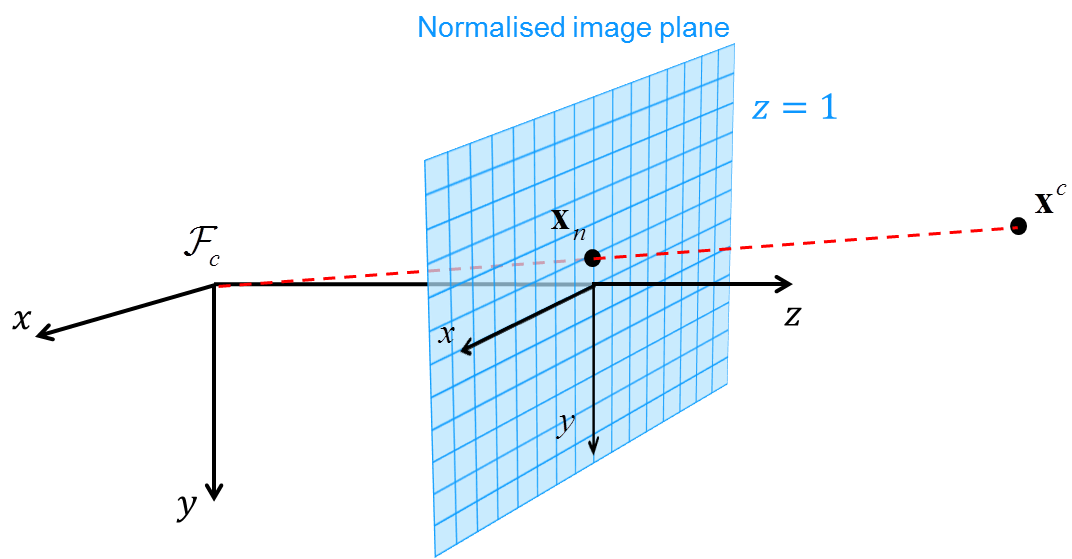
\includegraphics[height=5.5cm]{figures/perspective-camera-model_normalised.png}
    \caption{The normalised image plane is set at $z=1$ in front of the projective centre.
    This represents the perspective camera model for an idealised camera with $f = 1$.
    The point where the $z$-axis of $\cF_c$ intersects the normalised image plane is called the principal point.
    The central projection of the 3D point $\vecx^c$ onto the normalised image plane is the point $\vecx_n$, which is called the normalised image coordinate.
    }
    \label{fig:perspective-camera-model_normalised}
\end{figure}
%
We can project $\vecx^c$ onto the normalised image plane with the homogeneous \emph{perspective projection} matrix $\matPi_0$, by
\begin{equation}
  \tilde{\vecx}_n = \matPi_0 \tilde{\vecx}^c =
  \begin{bmatrix}
    1 & 0 & 0 & 0\\
    0 & 1 & 0 & 0\\
    0 & 0 & 1 & 0
  \end{bmatrix}
  \tilde{\vecx}^c = \vecx^c.
\end{equation}
On normalised form, we have that
\begin{equation} \label{eq:normalised-normalised-coordinate}
  \breve{\vecx}_n = 
  \begin{bmatrix}
    x_n\\
    y_n\\
    1
  \end{bmatrix} = 
  \begin{bmatrix}
    x^c / z^c\\
    y^c / z^c\\
    1
  \end{bmatrix}
  = \frac{1}{z^c}\vecx^c.
\end{equation}
The projected point $\tilde{\vecx}_n$ in the normalised image plane can be seen both as a Cartesian representation of the 3D point on the plane when normalised as in \eqref{eq:normalised-normalised-coordinate}, \emph{as well} as a homogeneous representation of the 2D point in the frame of the normalised image plane.
As illustrated in Figure~\ref{fig:perspective-camera-model_normalised}, this 2D frame is aligned with the $x$ and $y$ axes of the camera frame $\cF_c$, and its origin is at the \emph{principal point}, where the $z$-axis of $\cF_c$ intersects the plane.
Since $\vecx_n$ represents the image point for the idealised camera model, it is called the \emph{normalised image coordinate}, and we give it the special subscript $n$ notation.

\begin{figure}[htb]
    \centering
    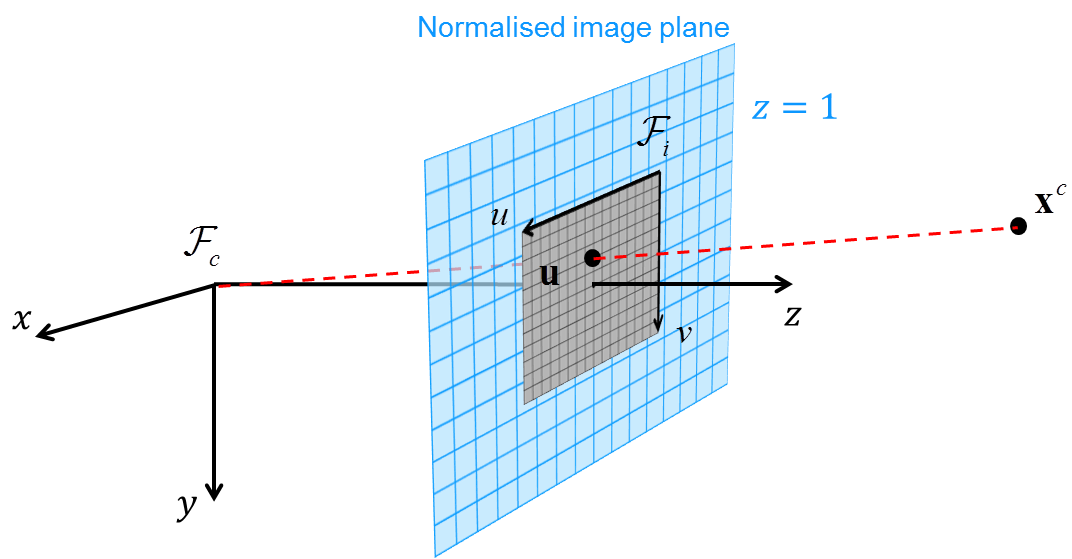
\includegraphics[height=5.5cm]{figures/perspective-camera-model.png}
    \caption{The image frame $\cF_i$, given in pixels, spans the normalised image plane.
    Its origin is at the upper-left corner of the image, its $u$-axis points right along the rows, and its $v$-axis points down along the columns.
    The mapping between normalised image coordinates and pixels is given by an affine transformation.
    }
    \label{fig:perspective-camera-model}
\end{figure}
%
As shown in Figure~\ref{fig:perspective-camera-model}, the image is represented by a 2D coordinate frame $\cF_i$ that spans the normalised image plane, with the origin at the upper-left corner of the image.
We recover the pixel coordinate $\vecu$ by mapping the normalised image coordinate $\tilde{\vecx}_n$ to the image frame $\cF_i$ with the affine transformation
\begin{equation}
  \tilde{\vecu} = \matK \tilde{\vecx}_n.
\end{equation}

The upper triangular matrix $\matK$ takes us from the idealised case to the camera-specific model.
It collects all parameters that are \emph{intrinsic} to a particular camera, and it is therefore known as the \emph{intrinsic matrix} or the \emph{calibration matrix}.
The affine transformation matrix is a combined scaling, shear and translation, and is given by
\begin{equation}
  \matK = 
  \begin{bmatrix}
    f_u & s_\theta & c_u\\
    0 & f_v & c_v\\
    0 & 0 & 1
  \end{bmatrix},
\end{equation}
where the elements of $\matK$ have the following geometric interpretation:
\begin{itemize}
  \item $f_u$ is the size of unit length in horizontal pixels.\\
  It can be expressed as $f_u = f s_u$, where $f$ is the focal length in metric units, and $s_u$ is the scaling factor that describes the horizontal pixel density in pixels per metric unit.
  \item $f_v$ is the size of unit length in vertical pixels.\\
  It can be expressed as $f_v = f s_v$, where $f$ is the focal length in metric units, and $s_v$ is the scaling factor that describes the vertical pixel density in pixels per metric unit.
  \item $c_u$ is the $u$-coordinate of the principal point in $\cF_i$.
  \item $c_v$ is the $v$-coordinate of the principal point in $\cF_i$.
  \item $s_\theta$ is the \emph{skew factor}, proportional to $\cot(\theta)$, where $\theta$ is the angle between the $u$ and $v$ axes in $\cF_i$.
\end{itemize}
Because of the structure of $\matK$, we preserve the normalised form of the homogeneous coordinates through the transformation:
\begin{equation}
  \breve{\vecu} = \matK \breve{\vecx}_n.
\end{equation}
We can estimate a calibration matrix $\matK$ by performing a camera calibration procedure such as \cite{Zhang2000ACalibration}.
It is common practise to reduce the number of parameters by dropping the skew factor.

When $\matK$ is known, we can obtain the \emph{calibrated} normalised image coordinates from the pixel $\vecu$ by applying the inverse transformation
\begin{equation}
  \tilde{\vecx}_n = \matK^{-1} \tilde{\vecu}.
\end{equation}
The inverse transformation also preserves the normalised form:
\begin{equation} \label{eq:normalised-from-pixel}
  \breve{\vecx}_n = \matK^{-1} \breve{\vecu}.
\end{equation}

If we crop or resample images from a calibrated camera, these transformations can be encoded directly in the calibration matrix.
Since cropping corresponds to a possible translation of the principal point, and resampling corresponds to scaling, we can update the calibration matrix by applying the corresponding transformations to $\matK$.

\begin{example}[frametitle=Camera calibration matrix for downsampled images]
We calibrate a camera using $1600 \times 1200$ pixel images, and we get the following camera calibration matrix:
\begin{equation}
  \matK =
  \begin{bmatrix}
    100 &   0 & 800\\
      0 & 100 & 600\\
      0 &   0 &   1
  \end{bmatrix}.
\end{equation}
If we downscale our images with a scale factor $s = 0.5$ to $800 \times 600$ pixels, how should we modify $\matK$ in order for it to be a valid calibration matrix for the downsampled images?

Since the camera calibration matrix is an affine transformation that transforms points on the normalised image plane to pixels in the image, we can apply the scaling to $\matK$ with the homogeneous transformation matrix
\begin{equation}
    \matS_s = 
  \begin{bmatrix}
    s & 0 & 0\\
    0 & s & 0\\
    0 & 0 & 1
  \end{bmatrix}.
\end{equation}
This results in the camera calibration matrix
\begin{equation}
  \matK_{0.5} = \matS_{0.5} \matK = 
    \begin{bmatrix}
    0.5 & 0 & 0\\
    0 & 0.5 & 0\\
    0 & 0 & 1
  \end{bmatrix}
  \begin{bmatrix}
    100 &   0 & 800\\
      0 & 100 & 600\\
      0 &   0 &   1
  \end{bmatrix}
  =
  \begin{bmatrix}
    50 &   0 & 400\\
      0 & 50 & 300\\
      0 &   0 &   1
  \end{bmatrix}.
\end{equation}
\end{example}

Putting it all together, the perspective camera model on homogeneous form gives us the projection
\begin{equation}
  \tilde{\vecu} = \matK \matPi_0 \tilde{\vecx}^c = \matK \vecx^c =
  \begin{bmatrix}
    f_u & s_\theta & c_u\\
    0 & f_v & c_v\\
    0 & 0 & 1
  \end{bmatrix}
  \vecx^c,
\end{equation}
which first projects $\vecx^c$ onto the normalised image plane, and then applies a 2D affine transformation that maps points on the normalised image plane to pixels in the image frame $\cF_i$.
The equivalent projection function on Euclidean form is given by
\begin{equation} \label{eq:projection-function}
  \vecu = \pi_p(\vecx^c; \matK) =
  \begin{bmatrix}
    1 & 0 & 0 \\
    0 & 1 & 0 \\
  \end{bmatrix}
  \matK \frac{1}{z^c} \vecx^c =
  \renewcommand\arraystretch{2}
  \begin{bmatrix}
    f_u \dfrac{x^c}{z^c} + s_\theta \dfrac{y^c}{z^c} + c_u\\
    f_v \dfrac{y^c}{z^c} + c_v \\
  \end{bmatrix}.
\end{equation}
For normalised image coordinates, we have
\begin{equation} \label{eq:normalised-projection-function}
  \vecx_n = \pi_n(\vecx^c) =
  \begin{bmatrix}
    1 & 0 & 0 \\
    0 & 1 & 0 \\
  \end{bmatrix}
  \frac{1}{z^c} \vecx^c =
  \begin{bmatrix}
    x^c / z^c\\
    y^c / z^c \\
  \end{bmatrix}.
\end{equation}

From \eqref{eq:normalised-normalised-coordinate} and \eqref{eq:normalised-from-pixel} we get the corresponding backprojection function
\begin{equation}
  \vecx^c = \pi^{-1}_p(\vecu, z; \matK) = z \matK^{-1} \breve{\vecu} = z
  \renewcommand\arraystretch{2}
  \begin{bmatrix}
    \dfrac{u - c_u}{f_u} - \dfrac{s_\theta}{f_u} \cdot \dfrac{v - c_v}{f_v}\\
    \dfrac{v - c_v}{f_v}\\
    1
  \end{bmatrix}.
\end{equation}
For normalised image coordinates, we have
\begin{equation} \label{eq:normalised-backprojection-function}
  \vecx^c = \pi^{-1}_n(\vecx_n, z) = z \breve{\vecx}_n = z
  \begin{bmatrix}
    x_n\\
    y_n\\
    1
  \end{bmatrix}.
\end{equation}

\begin{figure}[htb]
    \centering
    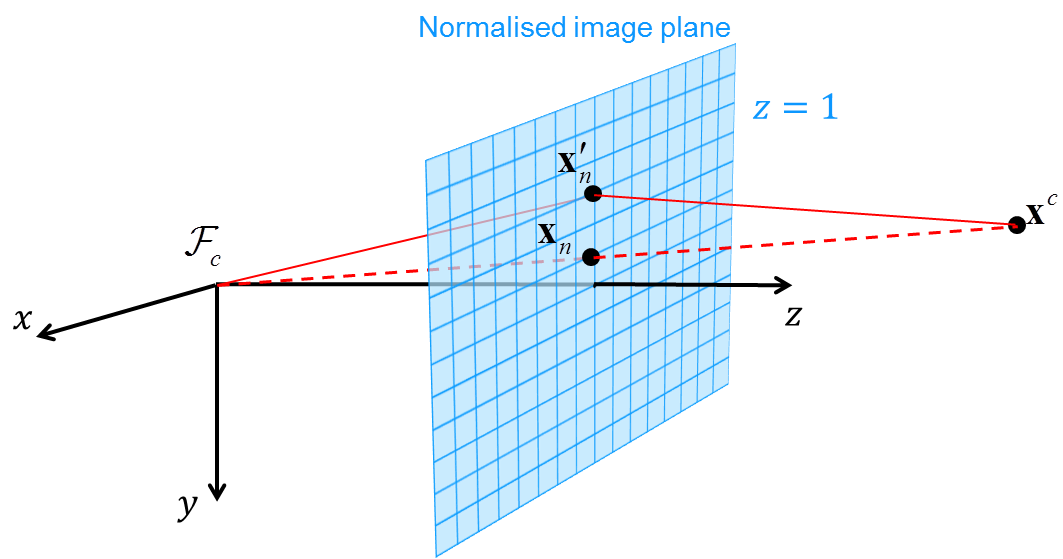
\includegraphics[height=5.5cm]{figures/radial-distortion.png}
    \caption{Typical cameras deviate from the perspective camera model geometry.
    A distortion model describes the relationship between undistorted points $\vecx_n$ and distorted points $\vecx'_n$ in the normalised image plane.
    By correcting for these deviations in the normalised image plane, the perspective camera model can still be applied in these situations.
    }
    \label{fig:radial-distortion}
\end{figure}
Practical cameras seldom fit perfectly with the perspective camera model, because they typically suffer from some kind of geometric distortion through the optical system.
This is illustrated in Figure~\ref{fig:radial-distortion}.
A \emph{distortion model} describes how a camera deviates from the perspective camera geometry, and is typically used to express the relationship between undistorted points $\vecx_n$ and distorted points $\vecx'_n$ in the normalised image plane.
A typical example is the \emph{radial distortion model}
\begin{align}
  r'{}^2 &= x'_n{}^2 + y'_n{}^2\\
  x_n &= x'_n (1 + k_1 r'{}^2 + k_2 r'{}^4)\\
  y_n &= y'_n (1 + k_1 r'{}^2 + k_2 r'{}^4),
\end{align}
where the parameters $k_1$ and $k_2$ can be estimated as part of the camera calibration process.

We will finish this discussion on geometric camera models by mentioning that there are several other models that may be more suitable than the perspective camera model in certain situations.
Examples include omnidirectional models \cite{Caruso2015Large-scaleCameras, Barreto2006UnifyingCameras} and models for underwater cameras \cite{uczynski2017TheHousings}.

\section{Epipolar geometry} \label{sec:epipolar-geometry}
\begin{figure}[htb]
    \centering
    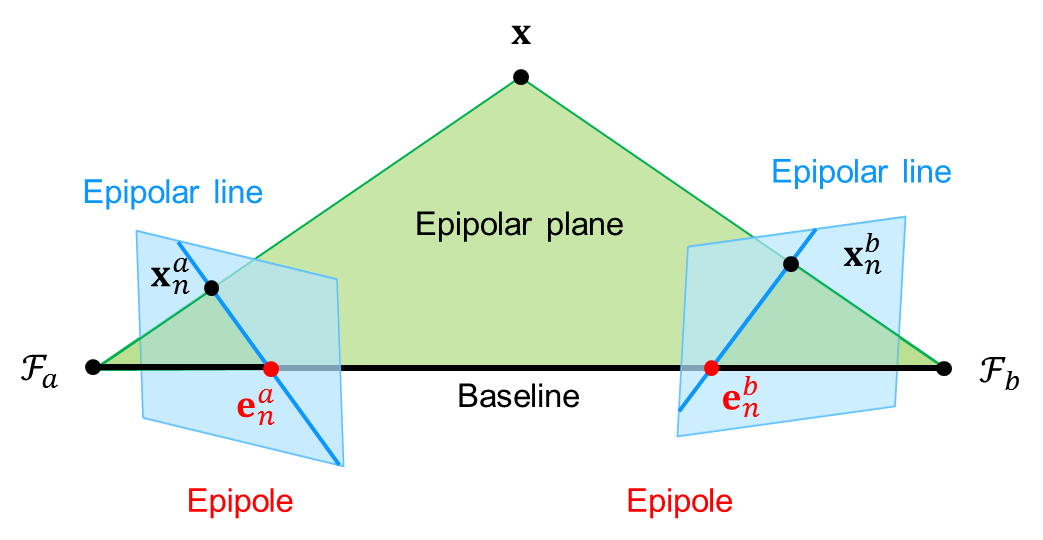
\includegraphics[width=0.75\columnwidth]{figures/epipolar-geometry.png}
    \caption{An illustration of the epipolar geometry between two perspective cameras, represented by the camera frames $\cF_a$ and $\cF_b$.
    The epipolar plane contains the point $\vecx$ and the two camera centres.
    The baseline is the line connecting the camera centres.
    The epipoles $\vece^a_n$ and $\vece^b_n$ are where the baseline intersects the image planes.
    The epipolar lines are where the epipolar plane intersects the image planes.
    Projected image points $\vecx^a_n$ and $\vecx^b_n$ corresponding to the same 3D point $\vecx$ must lie on the corresponding epipolar lines.
    This is called the epipolar constraint.
    }
    \label{fig:epipolar-geometry}
\end{figure}
Consider two perspective cameras, represented by the camera frames $\cF_a$ and $\cF_b$, as shown in Figure~\ref{fig:epipolar-geometry}.
The camera frames are related by the relative pose
\begin{equation} \label{eq:epipolar-pose-ab}
  \matT_{ab} =
  \begin{bmatrix}
    \matR_{ab} & \vect^a_{ab}\\
    \matr{0} & 1
  \end{bmatrix},
\end{equation}
or, equivalently, the inverse pose
\begin{equation}
  \matT_{ba} = \matT_{ab}^{-1} =
  \begin{bmatrix}
    \matR_{ba} & \vect^b_{ba}\\
    \matr{0} & 1
  \end{bmatrix}.
\end{equation}
Observing the same point $\vecx$ with these two cameras puts a strong geometric constraint on the point correspondence in the two images.
This constraint is called the \emph{epipolar constraint}.

Figure~\ref{fig:epipolar-geometry} shows the \emph{epipolar plane}, which is the plane containing the point $\vecx$ and the two camera centres of $\cF_a$ and $\cF_b$.
The line joining the camera centres is the \emph{baseline}, and the \emph{epipoles} are where the baseline intersects the image planes.
This means that the epipoles are the images of the other camera centre.
In normalised image coordinates, they are given by
\begin{align}
  \tilde{\vece}^a_n &= \vect^a_{ab}\\
  \tilde{\vece}^b_n &= \vect^b_{ba}.
\end{align}
Given the camera calibration matrices $\matK_a$ and $\matK_b$, the corresponding pixel points in the images are given by
\begin{align}
  \tilde{\vece}^a &= \matK_a \vect^a_{ab}\\
  \tilde{\vece}^b &= \matK_b \vect^b_{ba}.
\end{align}

\begin{figure}[htb]
    \centering
    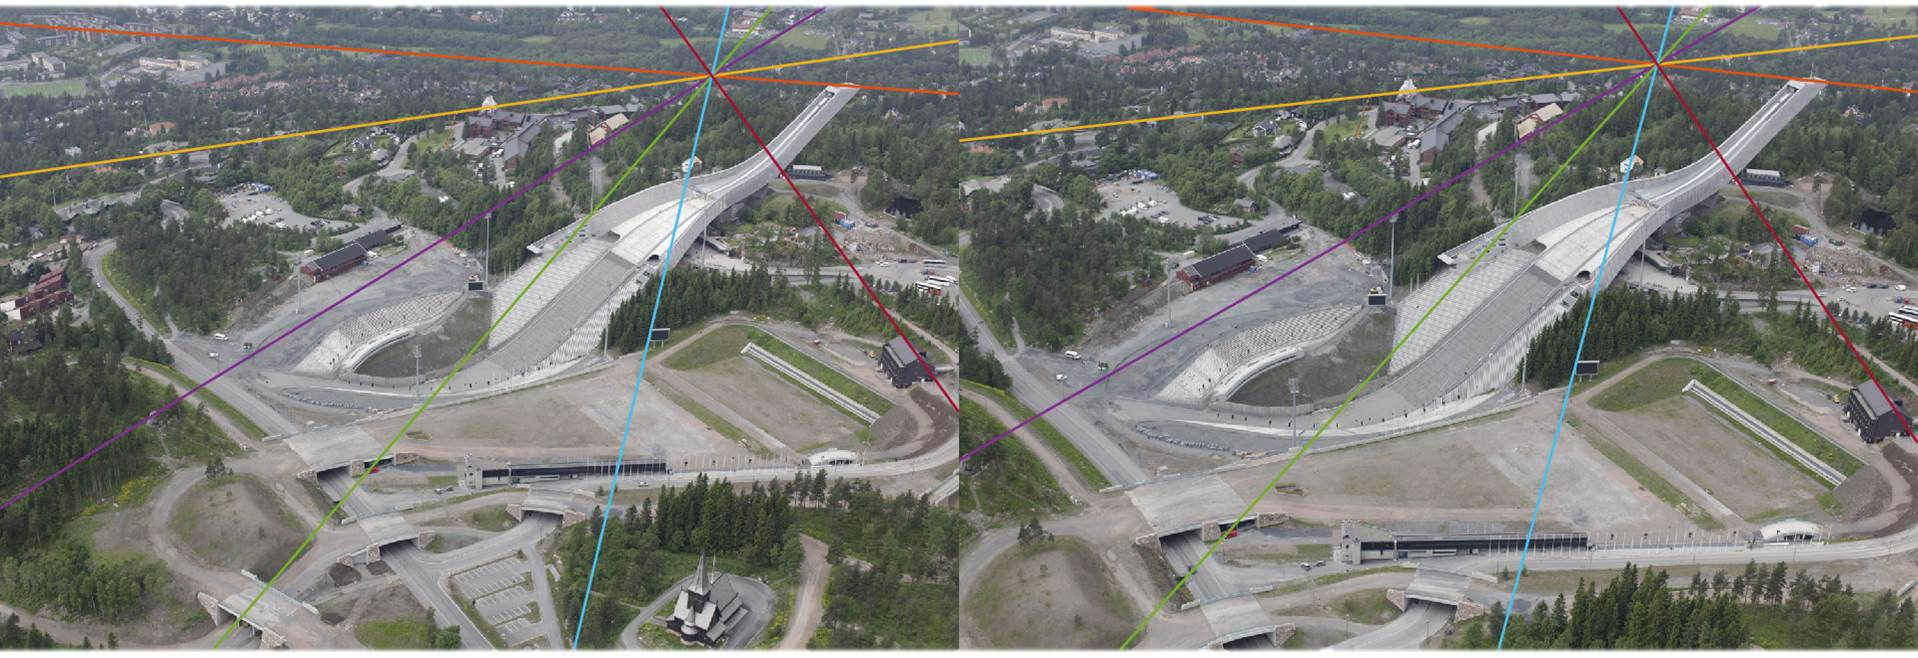
\includegraphics[width=\columnwidth]{figures/epipoles-example.jpg}
    \caption{An example of epipolar lines between two images that was captured sequentially while moving towards the Holmenkollen ski jump.
    In the left image, we see the epipolar lines intersect at the epipole, corresponding to the image of the camera centre in the second position (when the right image was captured).
    In the right image, we see the epipole corresponding to the the first camera position, projected in from behind.
    Corresponding epipolar lines are given the same colour.
    Notice that objects in the scene lie on corresponding epipolar lines, in accordance with the epipolar constraint.
    }
    \label{fig:epipoles-example}
\end{figure}
The lines where the epipolar plane intersects the image planes is called the \emph{epipolar lines}.
Informally, the epipolar constraint says that corresponding points in the two images \emph{must} lie on corresponding epipolar lines, since the cameras and the associated 3D point form a common epipolar plane.
Figure~\ref{fig:epipoles-example} shows a few examples of corresponding epipolar lines in two different images.


\begin{figure}[htb]
    \centering
    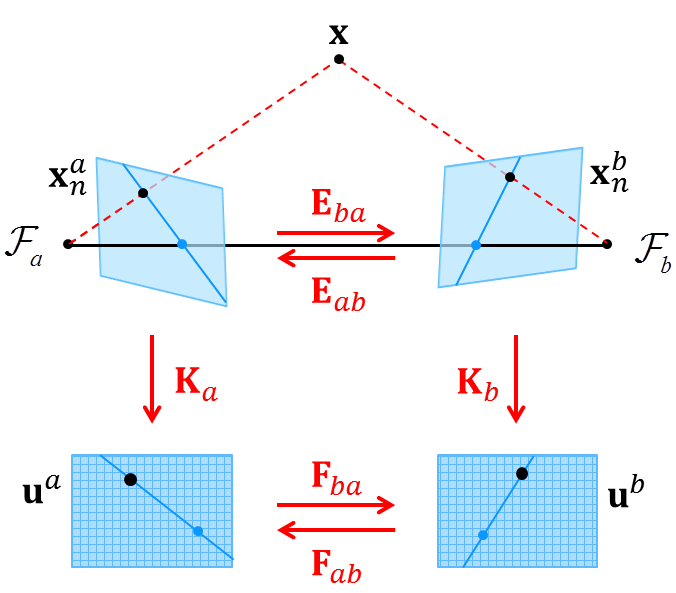
\includegraphics[width=0.5\columnwidth]{figures/essential-and-fundamental-matrices.png}
    \caption{The essential matrices $\matE_{ab}$ and $\matE_{ba}$ represent the epipolar constraint in the normalised image planes.
    The fundamental matrices $\matF_{ab}$ and $\matF_{ba}$ represent the same epipolar constraint in the images.
    They can be computed from the essential matrices via the camera calibration matrices $\matK_a$ and $\matK_b$.
    }
    \label{fig:essential-and-fundamental-matrices}
\end{figure}
The epipolar constraint can be represented mathematically by the \emph{essential matrix} $\matE \in \bbR^{3 \times 3}$ in the normalised image plane, and by the \emph{fundamental matrix} $\matF \in \bbR^{3 \times 3}$ in the image.
A correspondence $\vecx^a_n \leftrightarrow \vecx^b_n$ in the normalised image planes of the two cameras $\cF_a$ and $\cF_b$ must satisfy the equation
\begin{equation} \label{eq:essential-epipolar-constraint}
  \tilde{\vecx}^a_n{}\trans \matE_{ab} \tilde{\vecx}^b_n = 0.
\end{equation}
The essential matrix $\matE_{ab}$ is given by
\begin{equation} \label{eq:essential-structure}
  \matE_{ab} = \skewsymm{\vect^a_{ab}} \matR_{ab},
\end{equation}
which is related to the pose $\matT_{ab}$ in \eqref{eq:epipolar-pose-ab}.
The equation
\begin{equation}
  \tilde{\vecx}^b_n{}\trans \matE_{ba} \tilde{\vecx}^a_n = 0,
\end{equation}
with the essential matrix
\begin{equation}
  \matE_{ba} = \matE_{ab}\trans = \skewsymm{\vect^b_{ba}} \matR_{ba},
\end{equation}
is an equivalent representation of the constraint in \eqref{eq:essential-epipolar-constraint}.

As illustrated in Figure~\ref{fig:essential-and-fundamental-matrices}, the epipolar constraint extends naturally to pixel correspondences $\tilde{\vecu}^a \leftrightarrow \tilde{\vecu^b}$ via the camera calibration matrices $\matK_a$ and $\matK_b$.
The pixel correspondences must satisfy the equation
\begin{equation} \label{eq:fundamental-epipolar-constraint}
  \tilde{\vecu}^a{}\trans \matF_{ab} \tilde{\vecu}^b = 0,
\end{equation}
where the fundamental matrix $\matF_{ab}$ is given by
\begin{equation}
  \matF_{ab} = \matK_a\invtrans \matE_{ab} \matK_b^{-1}.
\end{equation}
The equivalent fundamental matrix $\matF_{ba}$ is similarly given by
\begin{equation}
    \matF_{ba} = \matF_{ab}\trans = \matK_b\invtrans \matE_{ba} \matK_a^{-1}.
\end{equation}

\begin{figure}[htb]
    \centering
    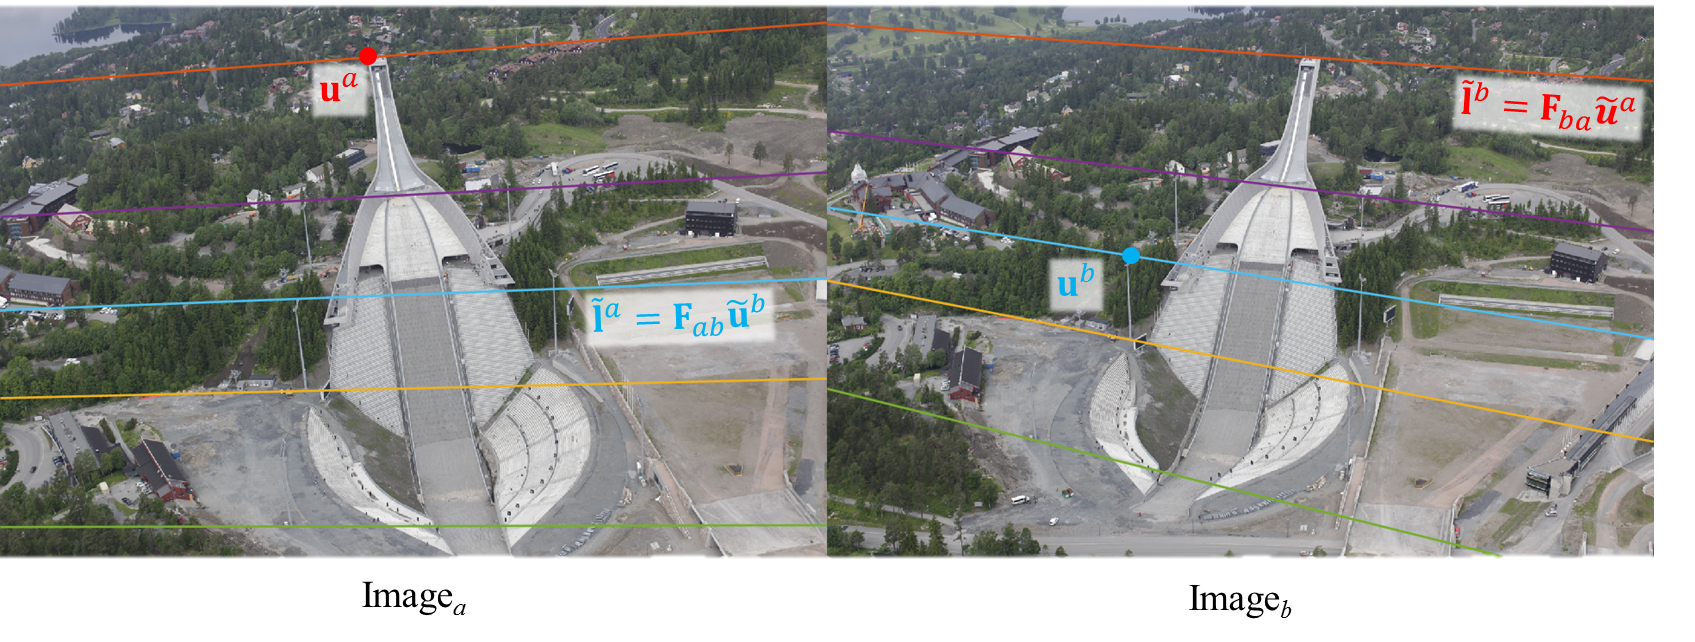
\includegraphics[width=\columnwidth]{figures/epipolar-lines-example.png}
    \caption{An example of computing epipolar lines in one image, given a point in the other image and the fundamental matrix.
    Corresponding epipolar lines are given the same colour.
    Notice that objects in the scene lie on corresponding epipolar lines in the images.
    }
    \label{fig:epipolar-lines-example}
\end{figure}
Since
\begin{equation}
  \tilde{\vecx}\trans \tilde{\vecl} = 0, \qquad \tilde{\vecl} =
  \begin{bmatrix}
    a\\
    b\\
    c
  \end{bmatrix}
  \in \bbP^2
\end{equation}
is the homogeneous representation of the line
\begin{equation}
  ax + by + c = 0,
\end{equation}
we see from \eqref{eq:essential-epipolar-constraint} that
\begin{equation}
  \tilde{\vecl}^a_n = \matE_{ab} \tilde{\vecx}^b_n
\end{equation}
is the epipolar line in the normalised image plane of $\cF_a$ corresponding to the point $\tilde{\vecx}^b_n$ in $\cF_b$.
Equivalently, we see from \eqref{eq:fundamental-epipolar-constraint} that
\begin{equation}
  \tilde{\vecl}^a = \matF_{ab} \tilde{\vecu}^b
\end{equation}
is the corresponding epipolar line in the image of $\cF_a$.
As illustrated in Figure~\ref{fig:epipolar-lines-example}, we can find the corresponding epipolar lines in $\cF_b$ by using $\matE_{ba}$ and $\matF_{ba}$.

We can restrict the search for correspondences by traversing along the epipolar line.
Given a set of putative point correspondences, we can test their validity by computing the distances to their corresponding epipolar lines.
The distance $d(\tilde{\vecu}, \tilde{\vecl})$ between a homogeneous point $\tilde{\vecu}$ and a homogeneous line $\tilde{\vecl}$ is given by
\begin{equation}
  d(\tilde{\vecu}, \tilde{\vecl}) = \frac{\tilde{\vecu}\trans \tilde{\vecl}}{\sqrt{{\tilde{l}_1}^2 + {\tilde{l}_2}^2}}.
\end{equation}
Although it is a necessary requirement that $d(\tilde{\vecu}^a, \matF_{ab} \tilde{\vecu}^b)$ is small for $\tilde{\vecu}^a$ and $\tilde{\vecu}^b$ to be a valid point correspondence, it important to emphasise that this is not sufficient to guarantee its validity.
It only suggests that the two points lie in the same epipolar plane.

We can estimate the fundamental matrix $\matF$ from point correspondences using the 7- or 8-point algorithms \cite{Hartley2004MultipleVision}.
The essential matrix $\matE$ can be estimated from point correspondences with the 5-point algorithm \cite{Nister2004AnProblem}.
We can also compute the essential matrix from the fundamental matrix by
\begin{align}
  \matE_{ab} = \matK_a\trans \matF_{ab} \matK_b.
\end{align}
We will see in Chapter~\ref{ch:estimating-pose-and-structure} that the structure of the essential matrix \eqref{eq:essential-structure} can be exploited to estimate the relative pose between images up to scale.

\begin{figure}[htb]
    \centering
    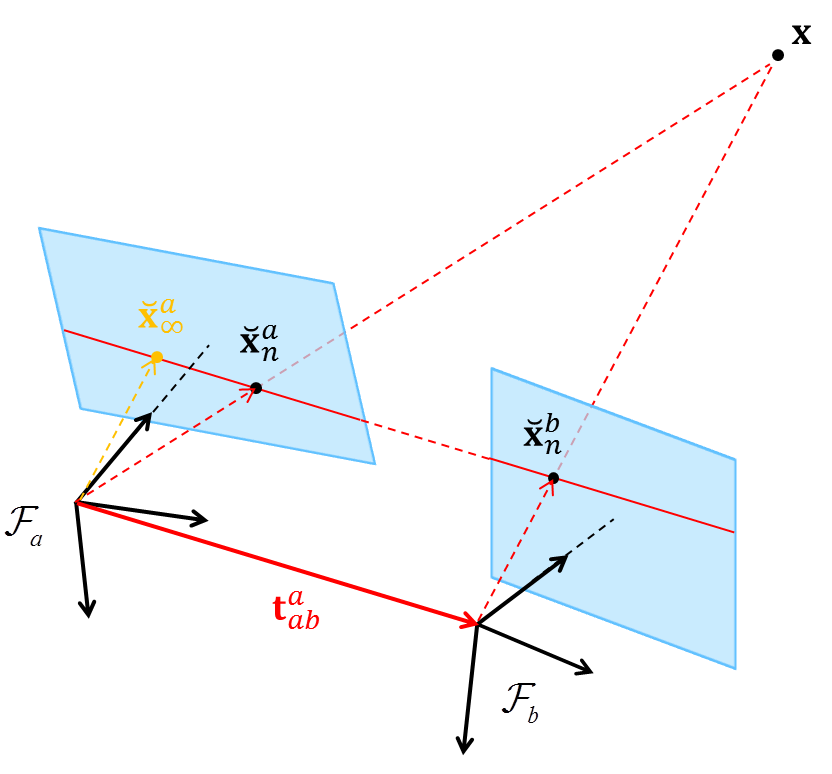
\includegraphics[width=0.6\columnwidth]{figures/epipolar-known-pose.png}
    \caption{When we know the pose of $\cF_b$ relative to $\cF_a$, we can map the image point $\breve{\vecx}^b_n$ into $\cF_a$ by $\tilde{\vecx}^a_{\infty} = \matR_{ab} \breve{\vecx}^b$.
    This corresponds to the image of $\vecx$ when $\vecx$ is infinitely far away.
    The point $\breve{\vecx}^a_n$ will in this example lie on the epipolar line to the right of $\tilde{\vecx}^a_{\infty}$ (in the direction of $\vect^a_{ab}$) for all other depths, restricting the search for valid correspondences further.
    }
    \label{fig:epipolar-known-pose}
\end{figure}
When the relative pose between the cameras are known, we can also express the epipolar line as a function of depth from the other camera.
This can for $\cF_a$ be expressed as as
\begin{equation} \label{eq:epipolar-line-known-pose-normalised}
  \tilde{\vecx}^a_n = \matR_{ab} \breve{\vecx}^b_n + \frac{1}{z^b} \vect^a_{ab},
\end{equation}
where $\breve{\vecx}^b_n$ is the normalised point correspondence in the normalised image plane of $\cF_b$ and $z^b$ is the depth from $\cF_b$.
Since we can think of $\breve{\vecx}^b_n$ as a 3D vector on the normalised image plane of $\cF_b$, the first term in \eqref{eq:epipolar-line-known-pose-normalised} rotates $\breve{\vecx}^b_n$ into the frame $\cF_a$ of the other camera (Figure~\ref{fig:epipolar-known-pose}).
These lines of sight are parallel, and correspond to the projections of a 3D point without observable depth.
This is because the motion between the cameras were without translation, or because the 3D point is ``infinitely'' far away.
We therefore write this projection as
\begin{equation}
  \tilde{\vecx}^a_{\infty} = \matR_{ab} \breve{\vecx}^b_n.
\end{equation}

The second term in \eqref{eq:epipolar-line-known-pose-normalised} moves $\tilde{\vecx}^a_n$ along the epipolar line defined by $\tilde{\vecx}^a_{\infty}$ and the epipole $\vect^a_{ab}$.
By increasing the \emph{inverse depth} $1/z^b$, we move away from $\tilde{\vecx}^a_{\infty}$, faster and faster as the depth decreases.

\begin{figure}[htb]
    \centering
    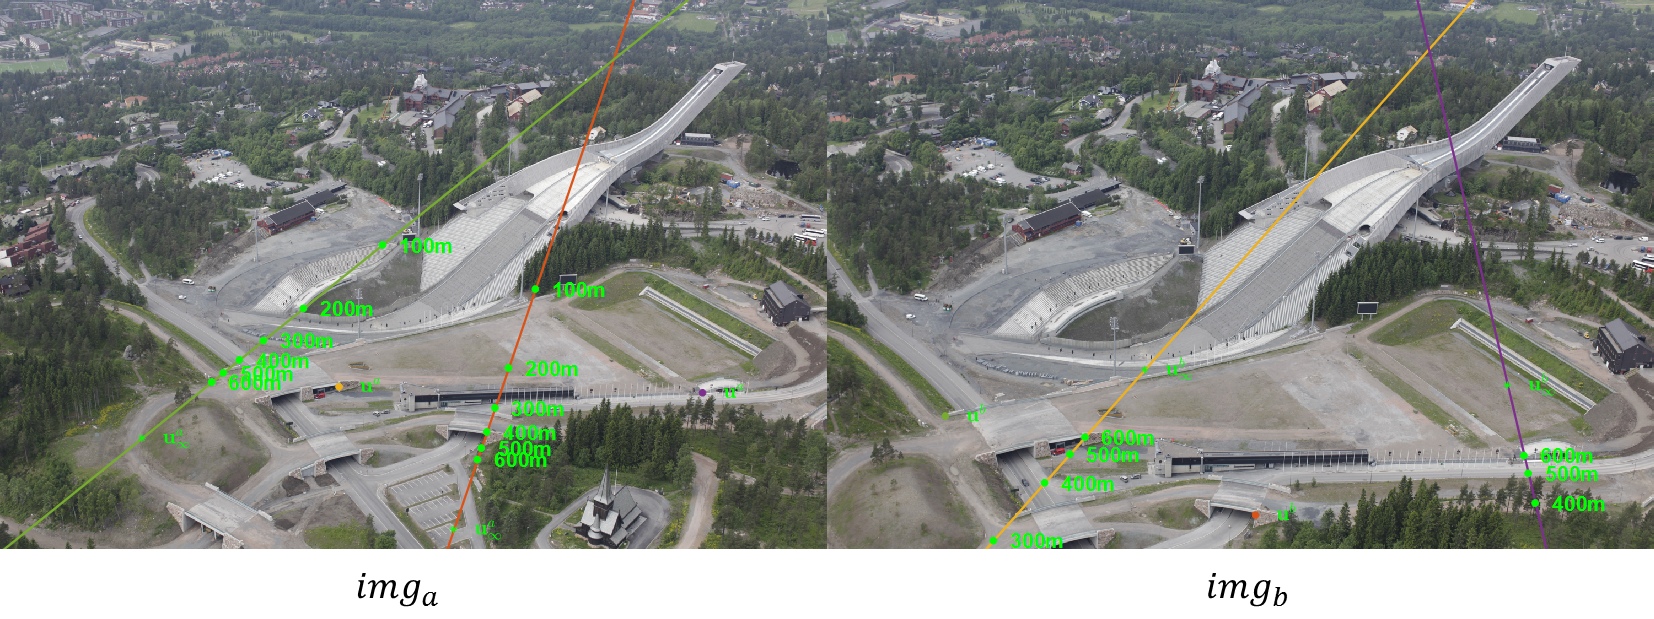
\includegraphics[width=\columnwidth]{figures/epipolar-range-example.png}
    \caption{Epipolar lines with depth.
    This example shows two chosen points in each image, with the corresponding epipolar lines in the other image given the same colour.
    The corresponding depth for the chosen points along the epipolar lines according to \eqref{eq:epipolar-line-known-pose-image} are shown, together with the limit at $\vecu_\infty$. 
    }
    \label{fig:epipolar-range-example}
\end{figure}
The corresponding representation of the epipolar line in the image is given by
\begin{equation} \label{eq:epipolar-line-known-pose-image}
\tilde{\vecu}^{a} = \tilde{\vecu}^a_{\infty} + \frac{1}{z^b}\matK_{a} \vect^a_{ab},
\end{equation}
with
\begin{equation}
  \tilde{\vecu}^a_{\infty} = \matK_a \matR_{ab} \matK^{-1}_b \breve{\vecu}^b
\end{equation}
The distance between the pixels 
\begin{equation}
  d = \norm{\vecu^a - \vecu^a_\infty}
\end{equation}
is called the \emph{disparity}, and is a measure of the observed parallax between the cameras.

\begin{example}[frametitle=Stereo geometry]
{
  \centering
  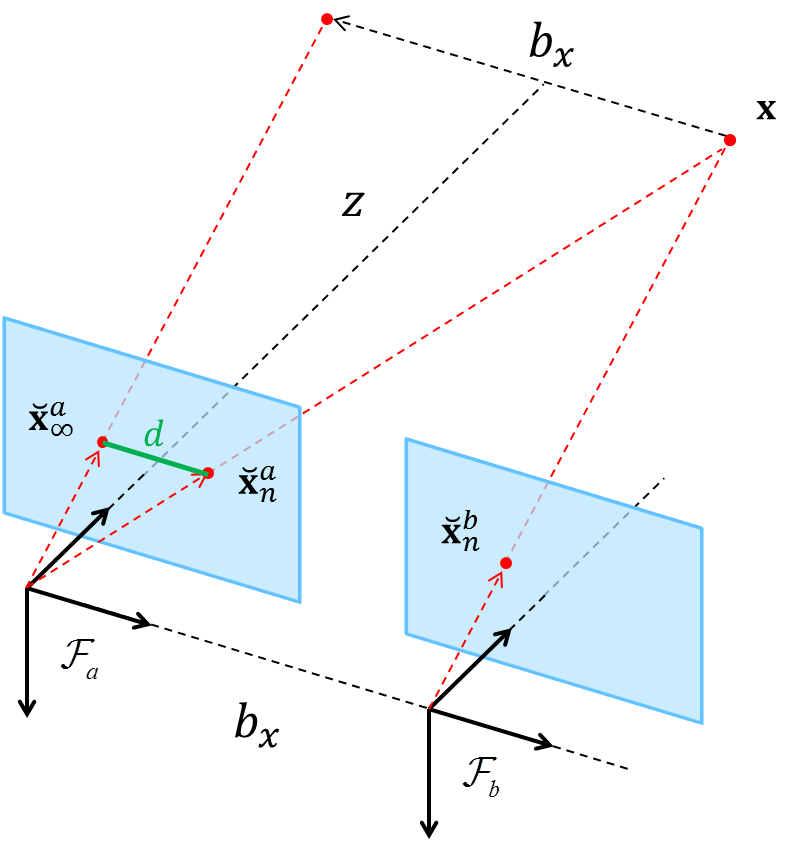
\includegraphics[width=0.6\columnwidth]{figures/stereo-geometry.png}
  \captionsetup{type=figure}
  \captionof{figure}{The ideal stereo geometry.
    The cameras have identical orientation, and baseline along the $x$-axis with distance $b_x$.}
  \label{fig:stereo-geometry}
  \par
}
Stereo imaging exploits a special case of the epipolar geometry presented in this section.
In stereo geometry
\begin{equation}
  \matK_a = \matK_b = \matK,
\end{equation}
\begin{equation}
  \matR_{ab} = \matR_{ba} = \matI, 
\end{equation}
and the translation between the cameras are typically along the $x$-axis
\begin{equation}
  \vect^a_{ab} = 
  \begin{bmatrix}
    b_x\\
    0\\
    0
  \end{bmatrix},
\end{equation}
where $b_x$ is the length of the baseline.
This means that the epipoles are at the infinity, 
\begin{equation}
  \breve{\vecu}^a_{\infty} = \breve{\vecu}^b,
\end{equation}
and the epipolar lines are horizontal along the rows in the images:
\begin{equation}
  \breve{\vecu}^{a} = \breve{\vecu}^b + 
  \renewcommand\arraystretch{1.5}
  \begin{bmatrix}
    f_u\dfrac{b_x}{z}\\
    0\\
    0
  \end{bmatrix}.
\end{equation}
The disparity is therefore given as
\begin{equation}
  d = \norm{\vecu^a - \vecu^a_\infty} = u^a - u^b = f_u\dfrac{b_x}{z}.
\end{equation}
This results in a simple expression for the depth given the disparity $d = u^a - u^b$:
\begin{equation}
  z = f_u\dfrac{b_x}{d}.
\end{equation}
\end{example}

We can use this representation of the epipolar lines to restrict the search for correspondences between images even further.
Clearly, the relevant part of the epipolar line can always be restricted on one end by $\tilde{\vecu}^a_{\infty}$ (or $\tilde{\vecx}^a_{\infty}$ on the normalised image plane), if it is visible in the image.
With information about the relevant interval of the depth $z^b$, we can use \eqref{eq:epipolar-line-known-pose-normalised} and \eqref{eq:epipolar-line-known-pose-image} to define the corresponding relevant segment on the epipolar line.
We will see in Chapter~\ref{ch:estimating-pose-and-structure} that this representation can also be used to estimate the depth to a point, given the relative pose and point correspondence.


\chapter{A brief introduction to Lie theory} \label{sec:Lie-theory}
In Chapter \ref{ch:3d-geometry} we saw that orientations and poses lie on manifolds in higher-dimensional spaces.
This makes it complicated to add increments, represent uncertainty and perform differentiation for such variables, since they do not have the same properties as vectors in vector spaces.

As an example, consider perturbing a rotation matrix $\matR \in \SO(3)$ by adding a matrix $\delta \matR \in \bbR^{3 \times 3}$.
This is problematic since for some $\delta \matR$ we have $\matR + \delta \matR \notin \SO(3)$, which means that the perturbation in general will not produce a new rotation matrix.
This also means that such perturbations is not a proper way to express the derivative of functions of rotation matrices.

We will in this chapter give a very brief introduction to a selection of extremely useful principles of \emph{Lie theory}.
The resulting mathematical framework will enable us to formulate estimation problems properly and with ease, by giving us the tools needed to work with rotations and poses \emph{on the manifold}.

Most of this chapter is heavily based on \cite{SolaARobotics}, as well as  \cite{Eade2013LieTransformations, barfoot2017state}.
It is meant as a practical introduction to the subject, and is not a proper introduction to the underlying theory as such.
Please see to the references above for more information.


\section{The Lie group}
\begin{figure}[htb]
    \centering
    \adjincludegraphics[width=0.5\columnwidth, trim={0 0 {.45\width} 0}, clip]{figures/manifold_tg.pdf}
    \caption{A manifold $\cM$ with the tangent vector space $\cT\cM_\cX$ at the point $\cX$. 
    In Lie groups, the manifold looks the same at every point, and all tangent spaces at any point are therefore alike.\\
    (Image source: \cite{SolaARobotics}; Cropped; licensed under \href{https://creativecommons.org/licenses/by-nc-sa/4.0/}{CC BY-NC-SA 4.0})}
    \label{fig:smooth-manifold}
\end{figure}
%
Informally, a Lie group is both a smooth differentiable manifold and a group satisfying the group axioms.
A group $(\cG, \circ)$ is a set $\cG$ with a composition operation $\circ$ that satisfies the axioms
\begin{align}
  \text{Closure under $\circ$} \; &: \quad \cX \circ \cY \in \cG\\
  \text{Identity $\cE$} \; &: \quad \cE \circ \cX = \cX \circ \cE = \cX \label{eq:lie-identity}\\
  \text{Inverse $\cX^{-1}$} \; &: \quad \cX^{-1} \circ \cX = \cX \circ \cX^{-1} = \cE\\
  \text{Associativity} \; &: \quad (\cX \circ \cY) \circ \cZ = \cX \circ (\cY \circ \cZ)
\end{align}
for elements $\cX, \cY, \cZ \in \cG$.

Lie groups can also transform elements of other sets.
Given a Lie group $\cM$ and a set $\cV$, we denote by $\cX \cdot v$ the \emph{action} of $\cX \in \cM$ on $v \in \cV$.
A group action must satisfy the axioms
\begin{align}
  \text{Identity} \; &: \quad \cE \cdot v = v\\
  \text{Compatibility} \; &: \quad (\cX \circ \cY) \cdot v = \cX \cdot (\cY \cdot v).
\end{align}

Since Lie groups are smooth manifolds, the group operations and actions are smooth, and look like operations on a vector space locally.
In fact, there is a unique tangent space at each point on the manifold that captures the local structure of the group (Figure~\ref{fig:smooth-manifold}).
This tangent space is a vector space that allows linear algebra and calculus.

In Lie groups, the local properties of smooth manifolds, which lets us do calculus, are combined with the global properties of groups, which lets us perform nonlinear composition and transformations on different objects.
We will in this chapter see how we can exploit these properties to perform perturbations and handle uncertainty on any element of the Lie group manifolds.
In Chapter~\ref{ch:jacobians} we will build upon this to define and compute derivatives on the manifolds. 

The orientation group $\SO(3)$ and pose group $\SE(3)$ introduced in chapter~\ref{ch:3d-geometry} are both examples of \emph{matrix Lie groups}.
These are Lie groups where the elements of the group are matrices, the composition operation is matrix multiplication, and the inversion operation is matrix inversion.
The action on vectors is $\matR \cdot \vecx \triangleq \matR \vecx$ for rotations $\matR \in \SO(3)$ and $\matT \cdot \vecx \triangleq \matR \vecx + \vect$ for poses $\matT \in \SE(3)$.
We will continue with a general introduction to Lie theory, before the properties of these groups are summarised in Sections \ref{sec:SO3_group} and \ref{sec:SE3_group}.


\section{The Lie algebra}
\begin{figure}[htb]
    \centering
    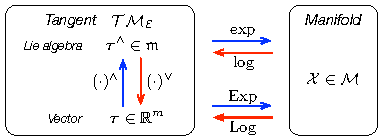
\includegraphics[width=0.8\columnwidth]{figures/maps.pdf}
    \caption{Mappings between the manifold $\cM$ and the representations of its tangent space at the identity $\cT \cM_\cE$.
    The hat $(\cdot)^\wedge$ and vee $(\cdot)^\vee$ operators map to/from the Lie algebra $\fm$ and tangent vector space $\bbR^m$. $\exp(\cdot)$ and $\log(\cdot)$ map the Lie algebra to/from the manifold, and $\Exp(\cdot)$ and $\Log(\cdot)$ are shortcuts to map the tangent vector space directly to/from $\cM$.\\
    (Image source: \cite{SolaARobotics}; licensed under \href{https://creativecommons.org/licenses/by-nc-sa/4.0/}{CC BY-NC-SA 4.0})}
    \label{fig:lie-maps}
\end{figure}
The structure of the tangent spaces on a Lie group manifold $\cM$ is the same everywhere.
We will denote the tangent space to $\cM$ at $\cX$ as $\cT \cM_\cX$, as illustrated in Figure~\ref{fig:smooth-manifold}.
The tangent space at the identity $\cT \cM_\cE$ is called the \emph{Lie algebra} of $\cM$, and is denoted $\fm$:
\begin{equation}
  \text{Lie algebra} \; : \quad \fm \triangleq \cT \cM_\cE.
\end{equation}

The Lie algebra $\fm$ is a vector space, and although its elements $\vectau^\wedge \in \fm$ can have non-trivial structures, they can be \emph{identified} with vectors $\vectau \in \bbR^m$, where $m$ is the dimensionality of $\cM$.
This is done by expressing $\vectau^\wedge$ as a linear combination of some base elements $\matE_i$, where $\matE_i$ are called the \emph{generators} of $\fm$.
We may in this way map between $\bbR^m$ to $\fm$ and vice versa with two mutually inverse linear maps called \emph{hat} and \emph{vee}:
\begin{align}
  \text{Hat:} \;& (\cdot)^\wedge : \bbR^m \to \fm ; \quad\quad \vectau^\wedge = \sum_{i = 1}^m \tau_i \matE_i\\
  \text{Vee:} \;& (\cdot)^\vee : \fm \to \bbR^m ; \quad\quad \vectau = (\vectau^\wedge)^\vee = \sum_{i = 1}^m \tau_i \vece_i,
\end{align}
where $\vece_i$ are the basis vectors of $\bbR^m$ so that $\vece^\wedge_i = \matE_i$ (Figure~\ref{fig:lie-maps}).
This lets us represent elements in the Lie algebra using vectors in a Cartesian vector space, which may be manipulated with linear algebra using matrix operations.


\section{The exponential map}
\begin{figure}[htb]
    \centering
    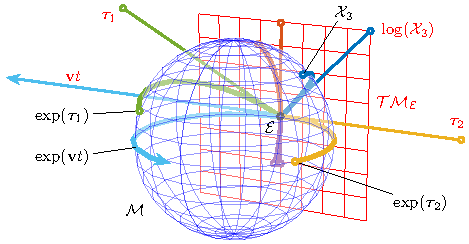
\includegraphics[width=0.9\columnwidth]{figures/exponential.pdf}
    \caption{An illustration of the relation between the Lie group and the Lie algebra.
    The Lie algebra $\cT\cM_\cE$ is the tangent space to the Lie group's manifold $\cM$ at the identity $\cE$.
    The exponential map wraps straight paths through the origin on the Lie algebra over the manifold along the corresponding geodesic.
    The logarithmic map unwraps curved and nonlinear paths on the manifold onto the linear Lie algebra.
    All points on the manifold has an exact equivalent on the tangent space.\\
    (Image source: \cite{SolaARobotics}; licensed under \href{https://creativecommons.org/licenses/by-nc-sa/4.0/}{CC BY-NC-SA 4.0})}
    \label{fig:lie-exponential}
\end{figure}
%
The \emph{exponential map} transfers elements of the Lie algebra $\vectau^\wedge \in \fm$ to elements of the group $\cX \in \cM$:
\begin{equation}
  \exp: \fm \to \cM; \quad\quad \cX = \exp(\vectau^\wedge).
\end{equation}
Intuitively, it wraps the tangent element over the manifold following the \emph{geodesic}, which in some sense is the shortest route along the manifold (Figure~\ref{fig:lie-exponential}).
The exponential map is \emph{exact} for all tangent elements, but does not always have a closed form expression.

The inverse transformation is the \emph{logarithmic map},
\begin{equation}
  \log: \cM \to \fm; \quad\quad \vectau^\wedge = \log(\cX),
\end{equation}
which unwraps elements on the manifold onto the tangent space (Figure~\ref{fig:lie-exponential}).

The \emph{capitalised exponential and logarithmic maps} are convenient compositions that lets us map vector elements $\vectau \in \bbR^m$ directly to group elements $\cX \in \cM$, and vice versa.
These are given by
\begin{alignat}{3}
  &\Exp: \bbR^m \to \cM; \quad\quad \cX &&= \Exp(\vectau) &&\triangleq \exp(\vectau^\wedge)\\
  &\Log: \cM \to \bbR^m; \quad\quad \vectau &&= \Log(\cX) &&\triangleq \log(\cX)^\vee.
\end{alignat}

Figure~\ref{fig:lie-maps} gives an overview of the different operators we can use to map between the manifold $\cM$ and the representations of its tangent space at the identity $\cT\cM_\cE$.
Additional properties of the exponential map is given in \cite{SolaARobotics, barfoot2017state}.

\section{Right and left perturbations} \label{sec:lie-right-left-perturbations}
The exponential map allows us to perform perturbations on elements $\cX$ on the manifold expressed as tangent space vectors $\vectau$ by combining one $\Exp$/$\Log$ operation with one composition.
Since the composition is non-commutative, the order of the operands is important for how the perturbations are performed.

With the combination
\begin{equation}
  \cX \circ \Exp(\prescript{\cX}{}{\vectau}),
\end{equation}
the perturbation is on the right side of the composition.
The tangent space vector $\prescript{\cX}{}{\vectau}$ therefore belongs to the tangent space at $\cX$, as denoted by the left superscript.
Following the convention we have used in Chapter~\ref{ch:3d-geometry}, we say that $\prescript{\cX}{}{\vectau}$ is expressed in the \emph{local} frame at $\cX$.

When we perform the perturbation on the left
\begin{equation}
 \Exp(\prescript{\cE}{}{\vectau}) \circ \cX,
\end{equation}
we have $\prescript{\cE}{}{\vectau} \in \cT\cM_\cE$, and we say that $\prescript{\cE}{}{\vectau}$ is expressed in the \emph{global} frame.

\begin{example}[frametitle=Local and global perturbations on poses] \label{ex:local-global-pert}
{
  \centering
  \adjincludegraphics[width=0.9\columnwidth, trim={{.1\width} {.25\height} {.15\width} {.15\height}}, clip]{figures/perturbation_illustration.pdf}
  \captionsetup{type=figure}
  \captionof{figure}{A world frame $\cF_w$ and a camera frame $\cF_c$. 
  A perturbation along the $x$-axis is performed on the right- and left-hand sides of the pose $\matT_{wc}$. 
  This corresponds to perturbations locally in the camera frame, and globally in the world frame, respectively.}
  \label{fig:perturbation-example}
  \par
}
The pose of a camera relative to the world frame is expressed as $\matT_{wc}$.
Perturbations on the right side of $\matT_{wc}$ are performed in the local camera coordinate frame, \emph{before} the transformation between the coordinate frames.
Perturbations on the left side are performed in the global world coordinate frame, \emph{after} the transformation.

The tangent vector $\vecxi = \begin{bmatrix}2 & 0 & 0 & 0 & 0 & 0\end{bmatrix}\trans$ corresponds to an increment of 2 units in the $x$-direction (see Section~\ref{sec:SE3_group}).
Figure~\ref{fig:perturbation-example} shows the result of perturbing $\matT_{wc}$ with $\vecxi$ locally along the $x$-axis of $\cF_c$ with $\matT_{wc}\Exp(\vecxi)$, and globally along the $x$-axis of $\cF_w$ with $\Exp(\vecxi)\matT_{wc}$.
\end{example}

We will in the following mostly consider local right side perturbations, although the left side convention is also common.
See \cite{SolaARobotics, barfoot2017state} for corresponding discussions covering left perturbations.


\section{Plus and minus operators} \label{sec:lie-plus-and-minus}
It is convenient to express right perturbations using the right plus and minus operators
\begin{alignat}{3}
  \cY &= \cX \oplus \prescript{\cX}{}{\vectau} &&\triangleq \cX \circ \Exp(\prescript{\cX}{}{\vectau}) &&\in \cM \label{eq:lie-plus-def}\\
  \prescript{\cX}{}{\vectau} &= \cY \ominus \cX &&\triangleq \Log(\cX^{-1} \circ \cY) &&\in \cT\cM_\cX. \label{eq:lie-minus-def}
\end{alignat}
The plus operator lets us increment an element $\cX$ with a tangent space vector $\prescript{\cX}{}{\vectau}$, while the minus operator lets us compute the corresponding tangent space vector between the two elements $\cX$ and $\cY$.
We will later use these operators to define derivatives on the manifold (Section~\ref{sec:derivative-Lie}).

It is also possible to define left plus and minus operators
\begin{alignat}{3}
  \cY &= \prescript{\cE}{}{\vectau} \oplus \cX &&\triangleq \Exp(\prescript{\cE}{}{\vectau}) \circ \cX &&\in \cM\\
  \prescript{\cE}{}{\vectau} &= \cY \ominus \cX &&\triangleq \Log(\cY \circ \cX^{-1}) &&\in \cT\cM_\cE.
\end{alignat}
Notice that while left and right $\oplus$ are distinguished by the operands, $\ominus$ is ambiguous.
Since we mostly consider right perturbations, we will also use the right definitions of $\oplus$ and $\ominus$ as default.

\begin{example}[frametitle=Interpolation on the manifold]
We can interpolate between two vectors $\vecx_1$ and $\vecx_2$ with the linear interpolation scheme
\begin{equation} \label{eq:vec-interp-example}
  \vecx = (1-\alpha) \vecx_1 + \alpha \vecx_2, \quad \alpha \in [0,1].
\end{equation}
This scheme will not work in general for Lie groups, since not all Lie groups are closed under addition.
For poses $\matT_1, \matT_2 \in \SE(3)$ for example, we will get
\begin{equation}
  (1-\alpha) \matT_1 + \alpha \matT_2 \notin \SE(3)
\end{equation}
for some values of $\alpha \in [0,1]$.

We can instead define a proper interpolation scheme on the manifold using Lie algebra.
The tangent vector between $\cX_1$ and $\cX_2$ in $\cT\cM_{\cX_1}$ is given by $\cX_2 \ominus \cX_1$.
The interpolation scheme
\begin{subequations}
\begin{align}
  \cX &= \cX_1 \oplus \alpha(\cX_2 \ominus \cX_1)\\
  &= \cX_1 \circ \Exp(\alpha \Log(\cX_1^{-1} \circ \cX_2))
\end{align}
\end{subequations}
will therefore move steadily along the geodesic from $\cX_1$ to $\cX_2$.

{
  \centering
  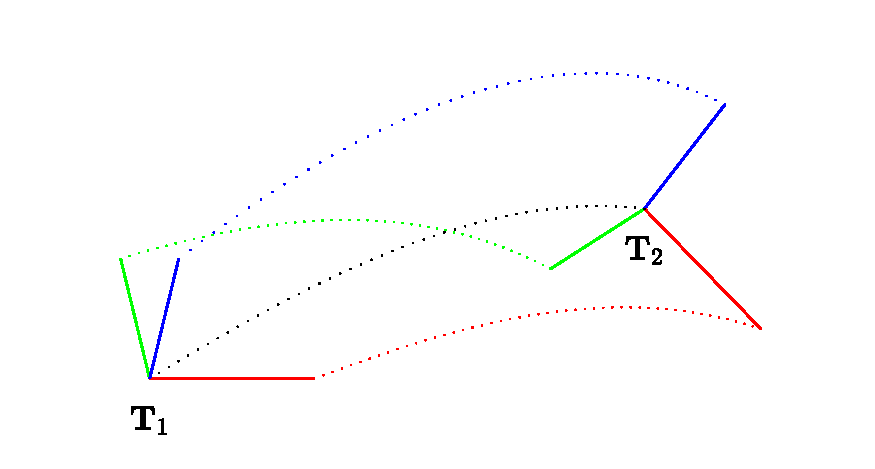
\includegraphics[width=0.75\columnwidth]{figures/pose_interpolation.pdf}
  \captionsetup{type=figure}
  \captionof{figure}{Interpolation along the manifold between two poses $\matT_1$ and $\matT_2$.}
  \label{fig:pose-interpolation}
  \par
}
For poses $\matT_1, \matT_2 \in \SE(3)$, we get
\begin{subequations}
\begin{align}
  \matT &= \matT_1 \circ \Exp(\alpha \Log(\matT_1^{-1} \circ \matT_2))\\
  &= \matT_1(\matT_1^{-1} \matT_2)^\alpha. \label{eq:pose-interp-example-exp}
\end{align}
\end{subequations}
An example of the interpolated motion along the manifold between two poses is shown in Figure~\ref{fig:pose-interpolation}.
We see that it follows a screw motion, corresponding to constant angular velocity, and constant translational velocity locally, so that the direction is constantly changed in the global frame.

{
  \centering
  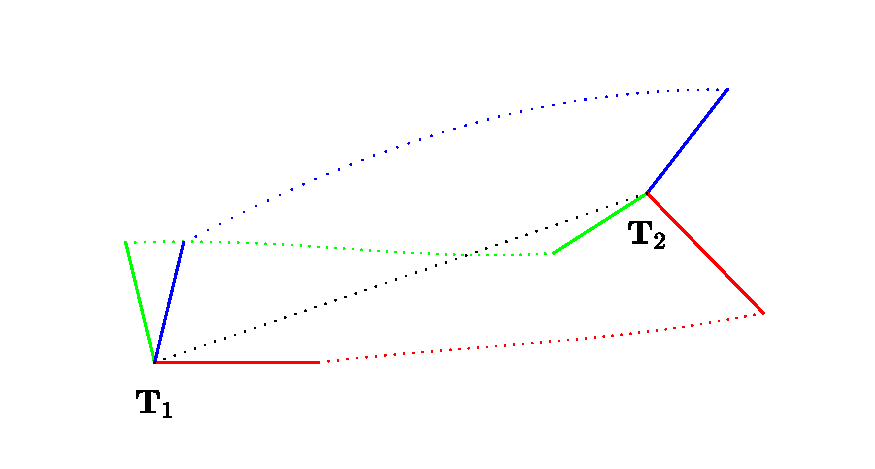
\includegraphics[width=0.75\columnwidth]{figures/pose_interpolation_hybrid.pdf}
  \captionsetup{type=figure}
  \captionof{figure}{Separate interpolation of rotation and position between two poses $\matT_1$ and $\matT_2$.}
  \label{fig:pose-interpolation-hybrid}
  \par
}
An alternative is to interpolate orientation and position separately (see the hybrid representation in Section~\ref{sec:hybrid-representation}).
For the poses $\matT_1 = \begin{bsmallmatrix} \matR_1 & \vect_1\\ \matr{0}\trans & 1 \end{bsmallmatrix}$ and $\matT_2 = \begin{bsmallmatrix} \matR_2 & \vect_2\\ \matr{0}\trans & 1 \end{bsmallmatrix}$, we get the separated interpolation scheme
\begin{align}
  \matR &= \matR_1 \oplus \alpha(\matR_2 \ominus \matR_1)\label{eq:rot-interp-example}\\ 
  \vect &= \vect_1 + \alpha(\vect_2 - \vect_1),
\end{align}
where the interpolated pose is given by $\matT = \begin{bsmallmatrix} \matR & \vect\\ \matr{0}\trans & 1 \end{bsmallmatrix}$, and we have rearranged \eqref{eq:vec-interp-example} a bit to show how similar the vector space and manifold schemes are.
Similarly to \eqref{eq:pose-interp-example-exp}, \eqref{eq:rot-interp-example} can also be expressed as $\matR = \matR_1(\matR_1\trans \matR_2)^\alpha$.
This separated scheme results in the linear translation motion shown in Figure~\ref{fig:pose-interpolation-hybrid}.
\end{example}

\section{The adjoint}
\begin{figure}[htb]
    \centering
    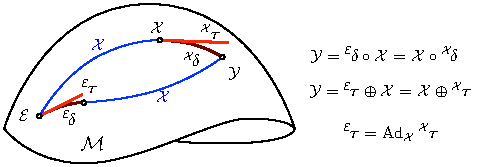
\includegraphics[width=0.75\columnwidth]{figures/adjoint.pdf}
    \caption{Two compositions $\cX \circ \prescript{\cX}{}{\delta}$ and $\prescript{\cE}{}{\delta} \circ \cX $ join the identity $\cE$ with the element $\cY$.
    Due to non-commutativity, the elements $\prescript{\cX}{}{\delta}$ and $\prescript{\cE}{}{\delta}$ are not equal.
    The corresponding tangent space vectors $\prescript{\cX}{}{\vectau} = \Log(\prescript{\cX}{}{\delta})$ and $\prescript{\cE}{}{\vectau} = \Log(\prescript{\cE}{}{\delta})$ are related by $\prescript{\cE}{}{\vectau} = \mAd_\cX \prescript{\cX}{}{\vectau}$, where $\mAd_\cX$ is the adjoint matrix of $\cM$ at $\cX$.\\
    (Image source: \cite{SolaARobotics}; licensed under \href{https://creativecommons.org/licenses/by-nc-sa/4.0/}{CC BY-NC-SA 4.0})}
    \label{fig:adjoint}
\end{figure}
%
In Section~\ref{sec:lie-right-left-perturbations} we saw that there are two natural ways of perturbing an element $\cX$ on the manifold by a tangent vector.
We can either right-perturb by a vector of the local tangent space, $\cX \circ \Exp(\prescript{\cX}{}{\vectau})$, or we can left-perturb by a vector of the tangent space at the identity, $\Exp(\prescript{\cE}{}{\vectau}) \circ \cX$.
One can show that this duality induces a relationship between the two tangent spaces called the \emph{adjoint of $\cM$ at $\cX$}, denoted by $\Ad_\cX$.

The \emph{adjoint action} of a group on its own Lie algebra is defined as
\begin{equation} \label{eq:adjoint}
  \Ad_\cX: \fm \to \fm; \quad\quad \Ad_\cX(\vectau^\wedge) \triangleq \cX \vectau^\wedge \cX^{-1}.
\end{equation}
As illustrated in Figure~\ref{fig:adjoint}, the adjoint determines a relation between the local and global tangent elements
\begin{equation}
  \prescript{\cE}{}{\vectau}^\wedge = \Ad_\cX(\prescript{\cX}{}{\vectau}^\wedge),
\end{equation}
so that 
\begin{equation}
  \prescript{\cE}{}{\vectau}^\wedge \oplus \cX = \cX \oplus \prescript{\cX}{}{\vectau}^\wedge.
\end{equation}

$\Ad_\cX()$ is a linear transformation, so we can define an equivalent matrix operator that maps the tangent vectors directly:
\begin{equation}
  \mAd_\cX: \bbR^m \to \bbR^m; \quad\quad \prescript{\cE}{}{\vectau} = \mAd_\cX \prescript{\cX}{}{\vectau}.
\end{equation}
The matrix $\mAd_\cX$ is called the \emph{adjoint matrix}, and it lets us linearly transform vectors of the tangent space at $\cX$ onto vectors of the tangent space at the identity $\cE$, corresponding to the same perturbation of $\cX$.
The adjoint matrix can be computed by applying the vee operator to \eqref{eq:adjoint}, so that
\begin{equation} \label{eq:adjoint-matrix}
  \mAd_\cX \triangleq (\cX \vectau^\wedge \cX^{-1})^\vee.
\end{equation}

Additional properties of the adjoint matrix is given in \cite{SolaARobotics, barfoot2017state}.

\begin{example}[frametitle=Computing global from local and vice versa]
In Example~\ref{ex:local-global-pert} we experienced the difference between applying a perturbation $\vecxi = \begin{bmatrix}2 & 0 & 0 & 0 & 0 & 0\end{bmatrix}\trans$ to the pose $\matT_{wc}$ locally on the right, and globally on the left.
The results are shown in Figure~\ref{fig:perturbation-example}.
We can use the adjoint matrix for poses $\mAd_\matT$ (see Section~\ref{sec:SE3_group}) to compute the corresponding perturbations in the other frame.

When $\vecxi$ is applied locally on the right side, the corresponding global perturbation is given by
\begin{equation}
  \vecxi^w =
  \mAd_{\matT_{wc}} \vecxi = 
  \begin{bmatrix} 0 & 2 & 0 & 0 & 0 & 0 \end{bmatrix}\trans,
\end{equation}
which is an increment of 2 units along the $y$-axis of $\cF_w$.

When $\vecxi$ is applied globally on the left side, we can use the inverse pose to compute the corresponding local perturbation by
\begin{equation}
  \vecxi^c =
  \mAd_{\matT_{wc}^{-1}} \vecxi = 
  \begin{bmatrix} 0 & \sqrt{2} & -\sqrt{2} & 0 & 0 & 0 \end{bmatrix}\trans,
\end{equation}
which is an increment of $\sqrt{2}$ units along the $y$-axis of $\cF_c$ and $-\sqrt{2}$ units along the $z$-axis of $\cF_c$.

We can use the adjoint matrix to transform tangent space vectors between coordinate frames, in the same way that we use poses to transform points.
\end{example}

\section{The 3D rotation group \SO(3)} \label{sec:SO3_group}
The \emph{special orthogonal group} in 3D is the set of valid rotation matrices
\begin{equation}
  \SO(3) = \left \{ \matR \in \bbR^{3 \times 3} \;\middle|\; \matR\matR\trans = \matI, \det \matR = 1 \right \},
\end{equation}
and is closed under matrix multiplication with identity $\matI$.
Inversion is achieved with transposition
\begin{equation}
  \matR^{-1} = \matR\trans,
\end{equation}
and composition with the product
\begin{equation}
  \matR_a \circ \matR_b = \matR_a \matR_b.
\end{equation}
The group action on vectors is given by the product
\begin{equation} \label{eq:SO3-group-action}
  \matR \cdot \vecx = \matR \vecx.
\end{equation}

\subsection{Lie algebra}
The Lie algebra of $\SO(3)$ is given by
\begin{equation}
  \so(3) = \left \{ \vectheta^\wedge = [\vectheta]_\times \in \bbR^{3 \times 3} \;\middle|\; \vectheta \in \bbR^3 \right \},
\end{equation}
where the tangent space vector $\vectheta \triangleq \theta \vecu$ corresponds to the rotation on angle-axis form, with angle $\theta$ and unit rotation axis $\vecu$ (see Section~\ref{sec:orientation}).
Since $\vectheta \in \bbR^3$, the dimension of $\SO(3)$ is $m = 3$.

The Lie algebra is a vector space that can be decomposed into
\begin{equation}
  \vectheta^\wedge = [\vectheta]_\times = \theta_1 \matE_1 + \theta_2 \matE_2 + \theta_3 \matE_3,
\end{equation}
where
\begin{equation}
  \matE_1 =
  \begin{bsmallmatrix}
    0 & 0 & 0\\
    0 & 0 & -1\\
    0 & 1 & 0
  \end{bsmallmatrix}, \;
  \matE_2 =
  \begin{bsmallmatrix}
    0 & 0 & 1\\
    0 & 0 & 0\\
    -1 & 0 & 0
  \end{bsmallmatrix}, \;
  \matE_3 =
  \begin{bsmallmatrix}
    0 & -1 & 0\\
    1 & 0 & 0\\
    0 & 0 & 0
  \end{bsmallmatrix},
\end{equation}
are the generators of $\so(3)$. The hat and vee operators are given by
\begin{align}
\begin{alignedat}{2}
  \text{Hat} \; &: \quad \vectheta^\wedge &&= [\vectheta]_\times\\
  \text{Vee} \; &: \quad \vectheta &&= [\vectheta]^\vee_\times.
\end{alignedat}
\end{align}

\subsection{Exp and Log maps} \label{sec:Exp-Log-SO3}
Since the tangent space vector $\vectheta = \theta \vecu$ corresponds to the axis-angle representation, the $\Exp$ map is simply the Rodrigues' rotation formula
\begin{equation} \label{eq:Exp-SO3}
  \matR = \Exp(\vectheta) \triangleq \matI + \sin \theta [\vecu]_\times + (1 - \cos \theta) [\vecu]^2_\times.
\end{equation}

The $\Log$ map is given by
\begin{equation} \label{eq:Log-SO3}
  \vectheta = \Log(\matR) \triangleq \frac{\theta}{2 \sin \theta} (\matR - \matR\trans)^\vee,
\end{equation}
where
\begin{equation}
  \theta = \arccos \left( \frac{\tr(\matR) - 1}{2} \right).
\end{equation}

Special care must be taken when $\theta$ is small.
Practical implementations can in these cases use a Taylor expansion of the coefficient $\theta / (2 \sin \theta)$ \cite{Eade2013LieTransformations}.
Also, when $\theta$ is small, the following approximation holds (see \eqref{eq:infinitesimal-rotaton}):
\begin{equation} \label{eq:SO3-Exp-approx}
  \matR = \Exp(\vectheta) \approx \matI + \vectheta^\wedge.
\end{equation}

\subsection{The adjoint}
The adjoint matrix for $\SO(3)$ at $\matR$ is given by
\begin{equation}
  \mAd_\matR = \matR  \in \bbR^{3 \times 3}.
\end{equation}

\section{The 3D rigid motion group \SE(3)} \label{sec:SE3_group}
The \emph{special Euclidean group} in 3D is the set of valid Euclidean transformation matrices
\begin{equation}
  \SE(3) = \left \{ \matT =
  \begin{bmatrix}
    \matR & \vect\\
    \matr{0}\trans & 1
  \end{bmatrix}
  \in \bbR^{4 \times 4} \;\middle|\; \matR \in \SO(3), \vect \in \bbR^3 \right \},
\end{equation}
and is closed under matrix multiplication with identity $\matI$.
Inversion is given by
\begin{equation}
  \matT^{-1} = 
  \begin{bmatrix}
    \matR\trans & -\matR\trans \vect\\
    \matr{0}\trans & 1
  \end{bmatrix},
\end{equation}
and composition with the product
\begin{equation}
  \matT_a \circ \matT_b = \matT_a \matT_b = 
  \begin{bmatrix}
    \matR_a \matR_b & \matR_a \vect_b + \vect_a\\
    \matr{0}\trans & 1
  \end{bmatrix}.
\end{equation}
The group action on vectors is given by
\begin{equation} \label{eq:SE3-group-action}
  \matT \cdot \vecx = \matT \tilde{\vecx} = \matR \vecx + \vect.
\end{equation}


\subsection{Lie algebra}
The Lie algebra of $\SE(3)$ is given by
\begin{equation}
  \se(3) = \left \{ \vecxi^\wedge = 
  \begin{bmatrix}
    [\vectheta]_\times & \vecrho\\
    \matr{0}\trans & 0
  \end{bmatrix}
  \in \bbR^{4 \times 4} \;\middle|\; \vecxi =
  \begin{bmatrix}
    \vecrho\\
    \vectheta
  \end{bmatrix}  
  \in \bbR^6 \right \},
\end{equation}
Since $\vecxi \in \bbR^6$, the dimension of $\SE(3)$ is $m = 6$.
The vectors $\vecrho, \vectheta \in \bbR^3$ correspond the translational and rotational parts, respectively.

The Lie algebra is a vector space that can be decomposed into
\begin{equation}
  \vecxi^\wedge = \xi_1 \matE_1 + \xi_2 \matE_2 + \xi_3 \matE_3 + \xi_4 \matE_4 + \xi_5 \matE_5 + \xi_6 \matE_6,
\end{equation}
where
\begin{equation}
\begin{alignedat}{3}
  &\matE_1 =
  \begin{bsmallmatrix}
    0 & 0 & 0 & 1\\
    0 & 0 & 0 & 0\\
    0 & 0 & 0 & 0\\
    0 & 0 & 0 & 0
  \end{bsmallmatrix}, \;
  &&\matE_2 =
  \begin{bsmallmatrix}
    0 & 0 & 0 & 0\\
    0 & 0 & 0 & 1\\
    0 & 0 & 0 & 0\\
    0 & 0 & 0 & 0
  \end{bsmallmatrix}, \;
  &&\matE_3 =
  \begin{bsmallmatrix}
    0 & 0 & 0 & 0\\
    0 & 0 & 0 & 0\\
    0 & 0 & 0 & 1\\
    0 & 0 & 0 & 0
  \end{bsmallmatrix},\\
  &\matE_4 =
  \begin{bsmallmatrix}
    0 & 0 & 0 & 0\\
    0 & 0 & -1 & 0\\
    0 & 1 & 0 & 0\\
    0 & 0 & 0 & 0
  \end{bsmallmatrix}, \;
  &&\matE_5 =
  \begin{bsmallmatrix}
    0 & 0 & 1 & 0\\
    0 & 0 & 0 & 0\\
    -1 & 0 & 0 & 0\\
    0 & 0 & 0 & 0
  \end{bsmallmatrix}, \;
  &&\matE_6 =
  \begin{bsmallmatrix}
    0 & -1 & 0 & 0\\
    1 & 0 & 0 & 0\\
    0 & 0 & 0 & 0\\
    0 & 0 & 0 & 0
  \end{bsmallmatrix},
\end{alignedat}
\end{equation}
are the generators of $\se(3)$. The hat and vee operators are given by
\begin{align}
\begin{alignedat}{2}
  \text{Hat} \; &: \quad \vecxi^\wedge &&= 
    \begin{bmatrix}
    [\vectheta]_\times & \vecrho\\
    \matr{0}\trans & 0
  \end{bmatrix}\\
  \text{Vee} \; &: \quad \vecxi &&=
    \begin{bmatrix}
    [\vectheta]_\times & \vecrho\\
    \matr{0}\trans & 0
  \end{bmatrix}^\vee.
\end{alignedat}
\end{align}

\subsection{Exp and Log maps}
The $\Exp$ map for $\SE(3)$ is given by
\begin{equation} \label{eq:SE3-exp}
  \matT = \Exp(\vecxi) \triangleq 
  \begin{bmatrix}
    \Exp(\vectheta) & \matV(\vectheta) \vecrho\\
    \matr{0}\trans & 1
  \end{bmatrix},  
\end{equation}
where $\Exp(\vectheta)$ is given by \eqref{eq:Exp-SO3} and 
\begin{equation}
  \matV(\vectheta) = \matI + \frac{1 - \cos \theta}{\theta}[\vecu]_\times + \frac{\theta - \sin \theta}{\theta} [\vecu]^2_\times.
\end{equation}

The $\Log$ map is given by
\begin{equation}
  \vecxi = \Log(\matT) \triangleq 
  \begin{bmatrix}
    \matV^{-1}(\vectheta) \vect\\
    \vectheta
  \end{bmatrix},
\end{equation}
where $\vectheta = \Log(\matR)$ from \eqref{eq:Log-SO3} and
\begin{equation}
  \matV^{-1}(\vectheta) = \matI - \frac{\theta}{2}[\vecu]_\times + \left(1 - \frac{\theta \sin \theta}{2(1 - \cos \theta)} \right)[\vecu]^2_\times.
\end{equation}

As for $\SO(3)$ in Section~\ref{sec:Exp-Log-SO3}, special care must be taken when $\theta$ is small \cite{Eade2013LieTransformations}.
Also, when $\theta$ is small, the following approximation holds:
\begin{equation} \label{eq:SE3-Exp-approx}
  \matT = \Exp(\vecxi) \approx \matI + \vecxi^\wedge.
\end{equation}

\subsection{The adjoint}
The adjoint matrix for $\SE(3)$ at $\matT$ is given by
\begin{equation}
  \mAd_\matT = 
  \begin{bmatrix}
    \matR & [\vect]_\times \matR\\
    \matr{0} & \matR
  \end{bmatrix} \in \bbR^{6 \times 6}.
\end{equation}

\subsection{Hybrid representation} \label{sec:hybrid-representation}
An alternative to representing poses on the $\SE(3)$ manifold, is to represent the orientation $\matR \in \SO(3)$ and position $\vect \in \bbR^3$ as two separate states without interaction.
Since $\vect$ is a vector, we will in this case only need to compute the $\Exp$ and $\Log$ maps for the orientation on the $\SO(3)$ manifold.

We can define maps the corresponding to $\Exp$ and $\Log$ for the hybrid representation as the pseudo-Exp and pseudo-Log maps \cite{BlancoAOptimization}:
\begin{align}
    \matT &= \text{pseudo-Exp}(\vecxi) \triangleq 
    \begin{bmatrix}
      \Exp(\vectheta) & \vecrho\\
      \matr{0}\trans & 1
  \end{bmatrix} \label{eq:SE3-pseudo-exp}\\ 
  \vecxi &= \text{pseudo-Log}(\matT) \triangleq 
  \begin{bmatrix}
    \vect\\
    \Log(\matR)
  \end{bmatrix}.
\end{align}

A \emph{retraction} is a more general way to define a mapping between the tangent space $\cT\cM$ and the manifold $\cM$ \cite{Forster2017, Dellaert2017, Absil2008OptimizationManifolds}.
For $\SE(3)$, the exponential map \eqref{eq:SE3-exp} is one example of retraction, while the pseudo-Exp \eqref{eq:SE3-pseudo-exp} is another, and sometimes more attractive choice.
This is because the pseudo-versions saves computations both for the $\Exp$ and $\Log$ maps, as well for the Jacobians, as we shall see in the next chapter.

\chapter{Jacobians} \label{ch:jacobians}
Problems in computer vision often involve nonlinear functions, such as camera projections and 3D transformations.
It is also common that these functions operate on and produce variables that are defined on manifolds, such as rotations on $\SO(3)$ and poses on $\SE(3)$.
As we will see in the following chapters, propagating uncertainty and estimating states from observations will typically involve linearising such functions with Taylor expansions.
Multivariate differentiation on vector spaces and Lie groups is therefore a key mathematical tool in vision-based state estimation.

This chapter will introduce useful notation and a procedure for computing derivatives on vector spaces and Lie groups based on \cite{SolaARobotics}.
We will finish this section with listing useful Jacobians for common operations on \SO(3) and \SE(3).

\section{Derivatives in vector spaces}
Let $f: \bbR^m \to \bbR^n$ be a multivariate function that takes vectors $\vecx \in \bbR^m$ as input and produces vectors $f(\vecx) \in \bbR^n$ as output.
The Jacobian matrix of $f$ is defined as the $n \times m$ matrix that stacks all the partial derivatives
%
\begin{equation} \label{eq:jacobian_def}
  \matJ = \dpar{f(\vecx)}{\vecx} \triangleq
  \begin{bmatrix}
    \dpar{f_1}{x_1} & \hdots & \dpar{f_1}{x_m}\\
    \vdots & & \vdots\\
    \dpar{f_n}{x_1} & \hdots & \dpar{f_n}{x_m}
  \end{bmatrix}
  \in \bbR^{n \times m}.
\end{equation}
%
Each column vector $\vecj_i = [\dpar{f_1}{x_i} \hdots \dpar{f_n}{x_i}]\trans$ of the Jacobian \eqref{eq:jacobian_def} corresponds to
%
\begin{equation} \label{eq:jacobian_column}
  \vecj_i = \dpar{f(\vecx)}{x_i} \triangleq \lim_{h \to 0} \frac{f(\vecx + h \vece_i) - f(\vecx)}{h} \in \bbR^n,
\end{equation}
%
where $\vece_i$ is the $i$-th natural basis vector of $\bbR^m$.
This represents the instantaneous variation of $f(\vecx)$ when $\vecx$ is perturbed in the direction of $\vece_i$.
We will in the following adopt the convenient notation from \cite{SolaARobotics}, where the Jacobian is given on the compact form
%
\begin{equation}  \label{eq:jacobian_sola_def}
  \matJ = \dpar{f(\vecx)}{\vecx} \triangleq
  \lim_{\vech \to 0} \frac{f(\vecx + \vech) - f(\vecx)}{\vech} \in \bbR^{n \times m},
\end{equation}
%
with $\vech \in \bbR^m$, which combines all the columns~\eqref{eq:jacobian_column} to form the definition of~\eqref{eq:jacobian_def}.
Like the Jacobian matrix in~\eqref{eq:jacobian_def}, the form used in~\eqref{eq:jacobian_sola_def} is just a notational convenience, since division by the vector $\vech$ is undefined, and proper computation requires~\eqref{eq:jacobian_column}.
However, by using this notation we can follow a straight-forward procedure to calculate Jacobians, by developing the numerator into a form linear in $\vech$ and identifying the left hand side as the Jacobian:
%
\begin{equation}  \label{eq:computing_jacobian}
  \lim_{\vech \to 0} \frac{f(\vecx + \vech) - f(\vecx)}{\vech} = \hdots =
  \lim_{\vech \to 0} \frac{\matJ \vech}{\vech} \triangleq \dpar{(\matJ \vech)}{\vech} = \matJ.
\end{equation}
%
To distinguish and identify different Jacobians, we will use the notation $\jac{f(\vecx)}{\vecx} \triangleq \dpar{f(\vecx)}{\vecx}$ and $\jac{\vecy}{\vecx} \triangleq \dpar{\vecy}{\vecx}$.

\begin{example}[frametitle=Computing the Jacobian $\jac{\matA \vecx}{\vecx}$]
For a vector $\vecx \in \bbR^m$ and a constant conformable matrix $\matA$, we want to compute the derivative of $f(\vecx) = \matA \vecx$ with respect to $\vecx$.
Using \eqref{eq:jacobian_sola_def} we get
\begin{subequations}
\begin{align}
  \jac{\matA \vecx}{\vecx} = \dpar{\matA \vecx}{\vecx} 
  &= \lim_{\vech \to 0} \frac{\matA (\vecx + \vech) - \matA \vecx}{\vech}\\[0.3em]
  &= \lim_{\vech \to 0} \frac{\matA \vecx + \matA \vech - \matA \vecx}{\vech}\\[0.3em]
  &= \lim_{\vech \to 0} \frac{\matA \vech}{\vech}\\[0.3em]
  &= \matA.
\end{align}
\end{subequations}
\end{example}

\begin{example}[frametitle=Computing the Jacobian $\jac{\vecx\trans \matA \vecx}{\vecx}$]
For a vector $\vecx \in \bbR^m$ and a constant matrix $\matA \in \bbR^{m \times m}$, we now want to compute the derivative of the scalar-valued quadratic form $f(\vecx) = \vecx\trans \matA \vecx$ with respect to $\vecx$.
By applying \eqref{eq:jacobian_sola_def} we get
\begin{subequations} \label{eq:jacobian_quadratic_form}
\begin{align}
  \jac{\vecx\trans \matA \vecx}{\vecx}
  &= \lim_{\vech \to 0} \frac{(\vecx + \vech)\trans \matA (\vecx + \vech) - \vecx\trans \matA \vecx}{\vech}\\
  &= \lim_{\vech \to 0} \frac{\vecx\trans \matA \vecx + \vech\trans \matA \vecx + \vecx\trans \matA \vech + \vech\trans \matA \vech - \vecx\trans \matA \vecx}{\vech}.\\
\intertext{By dropping the higher order term and using that for scalars $a\trans = a$, we get}
  \jac{\vecx\trans \matA \vecx}{\vecx}
  &= \lim_{\vech \to 0} \frac{\vecx\trans \matA \vech + (\vech\trans \matA \vecx)\trans}{\vech}\\[0.3em]
  &= \lim_{\vech \to 0} \frac{\vecx\trans \matA \vech + \vecx\trans \matA\trans \vech}{\vech}\\[0.3em]
  &= \lim_{\vech \to 0} \frac{\vecx\trans (\matA + \matA\trans) \vech}{\vech}\\[0.3em]
  &= \vecx\trans (\matA + \matA\trans).
\end{align}
\end{subequations}
\end{example}

For $\vecy = f(\vecx)$ and $\vecz = g(\vecy)$ we have $\vecz = g(f(\vecx))$.
The chain rule also applies in multivariate calculus, and lets us compute the derivative of $\vecz$ with respect to $\vecx$ as
\begin{equation}
  \dpar{\vecz}{\vecx} = \dpar{\vecz}{\vecy} \dpar{\vecy}{\vecx}.
\end{equation}
We can therefore express the Jacobian $\jac{\vecz}{\vecx}$ as a composition of several Jacobian blocks
\begin{equation}
  \jac{\vecz}{\vecx} = \jac{\vecz}{\vecy} \jac{\vecy}{\vecx}.
\end{equation}

\begin{example}[frametitle=Computing the Jacobian $\jac{\norm{\vecx - \veca}}{\vecx}$] \label{ex:jacobian-of-norm}
For a vector $\vecx \in \bbR^m$ and the constant vector $\veca \in \bbR^m$, we want to compute the derivative of the scalar-valued L2 norm of the difference between these vectors $f(\vecx) = \norm{\vecx - \veca}$ with respect to $\vecx$.
Using the chain rule, we can represent the Jacobian as
\begin{equation} \label{eq:jacobian_normdiff_blocks}
  \jac{\norm{\vecx - \veca}}{\vecx} = \jac{\norm{\vecx - \veca}}{\vecx - \veca} \jac{\vecx - \veca}{\vecx}.
\end{equation}
We can compute the first Jacobian by using the chain rule again:
\begin{equation}
  \jac{\norm{\vecx}}{\vecx} = \jac{\sqrt{\vecx\trans \vecx}}{\vecx\trans \vecx} \jac{\vecx\trans \vecx}{\vecx}.
\end{equation}
We can here recognise that $\jac{\sqrt{\vecx\trans \vecx}}{\vecx\trans \vecx}$ is simply $\dif{\sqrt{u}}{u}$ with $u = \vecx\trans \vecx$, and $\jac{\vecx\trans \vecx}{\vecx}$ is a special case of $\jac{\vecx\trans \matA \vecx}{\vecx}$ from \eqref{eq:jacobian_quadratic_form} with $\matA = \matI$.
This gives us
\begin{subequations} \label{eq:jacobian_norm}
\begin{align}
  \jac{\norm{\vecx}}{\vecx} 
  &= \jac{\sqrt{\vecx\trans \vecx}}{\vecx\trans \vecx} \jac{\vecx\trans \vecx}{\vecx}\\[0.3em]
  &= \frac{1}{2 \sqrt{\vecx\trans \vecx}} \; \vecx\trans(\matI + \matI\trans)\\[0.3em]
  &= \frac{2 \vecx\trans}{2 \norm{\vecx}}\\[0.3em]
  &= \frac{\vecx\trans}{\norm{\vecx}}.
\end{align}
\end{subequations}
By applying \eqref{eq:jacobian_sola_def} on the second Jacobian in \eqref{eq:jacobian_normdiff_blocks}, we see that
\begin{equation} \label{eq:jacobian_diff}
  \jac{\vecx - \veca}{\vecx} = \matI.
\end{equation}
We can now finally compose the Jacobian blocks \eqref{eq:jacobian_norm} and \eqref{eq:jacobian_diff} in \eqref{eq:jacobian_normdiff_blocks} to compute the desired Jacobian 
\begin{subequations} \label{eq:jacobian_normdiff}
\begin{align}
  \jac{\norm{\vecx - \veca}}{\vecx} 
  &= \jac{\norm{\vecx - \veca}}{\vecx - \veca} \jac{\vecx - \veca}{\vecx}\\[0.3em]
  &= \frac{(\vecx - \veca)\trans}{\norm{\vecx - \veca}} \; \matI\\[0.3em]
  &= \frac{(\vecx - \veca)\trans}{\norm{\vecx - \veca}}.
\end{align}
\end{subequations}
\end{example}

For small values of $\vech$, we have the linear first-order Taylor approximation
\begin{equation} \label{eq:linear-approximation}
  f(\vecx + \vech) \xrightarrow[\vech \to 0]{} f(\vecx) + \jac{f(\vecx)}{\vecx} \vech.
\end{equation}

This concludes our brief introduction to derivatives in vector spaces.
Those seeking further details should consult an appropriate text on multivariate calculus.
We will finish this section by emphasising that the procedure in \eqref{eq:jacobian_sola_def} is not applicable for 3D rotations and poses, which are defined on manifolds rather than on vector spaces.
The next section will describe how we apply the Lie theory from Chapter~\ref{sec:Lie-theory} to differentiate functions on these manifolds.

\section{Derivatives on Lie groups} \label{sec:derivative-Lie}
\begin{figure}[htb]
    \centering
    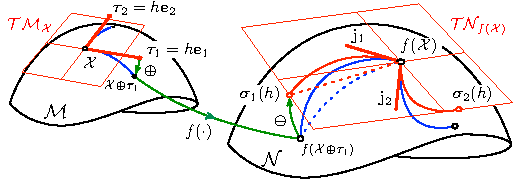
\includegraphics[width=0.9\columnwidth]{figures/jacobian.pdf}
    \caption{The right derivative of a function $f: \cM \to \cN$.
    The perturbation vectors in the canonical directions, $\vectau_i = h \vece_i \in \cT\cM_\cX$ are propagated to perturbation vectors $\vecsigma_i \in \cT\cN_{f(\cX)}$ through $\vecsigma_i(h) = f(\cX \oplus h \vece_i) \ominus f(\cX)$.
    The column vectors $\vecj_i$ of $\matJ$ are the derivatives $\vecj_i = \lim_{h \to 0} \vecsigma_i(h)/h$, and the Jacobian matrix $\matJ = [\vecj_1 \cdots \vecj_m]$ linearly maps tangent space vectors from $\cT\cM_\cX$ to $\cT\cN_{f(\cX)}$.\\
    (Image source: \cite{SolaARobotics}; licensed under \href{https://creativecommons.org/licenses/by-nc-sa/4.0/}{CC BY-NC-SA 4.0})}
    \label{fig:lie-jacobian}
\end{figure}

For functions acting on Lie groups, we can express the derivative similarly to that of \eqref{eq:jacobian_sola_def} by using the $\oplus$ and $\ominus$ operators from Section~\ref{sec:lie-plus-and-minus} with infinitesimal perturbations in the tangent space.
For a function $f : \cM \to \cN$, the right (local) derivative is given by
\begin{align}
  \jac{}{} = \frac{^{\cX} \partial f(\cX)}{\partial \cX} &\triangleq 
  \lim_{\vectau \to 0} \frac{f(\cX \oplus \vectau) \ominus f(\cX)}{\vectau} \in \bbR^{n \times m} \label{eq:lie-derivative}\\
  &= \lim_{\vectau \to 0} \frac{\Log \left( f(\cX)^{-1} \circ f(\cX \circ \Exp(\vectau)) \right)}{\vectau},
\end{align}
where $\vectau \in \cT\cM_\cX$.

Variations in $\cX$ and $f(\cX)$ are here expressed in terms of vectors in the local tangent spaces at $\cX \in \cM$ and $f(\cX) \in \cN$ respectively.
The tangent space vector
\begin{equation}
  \vecsigma_i(h) = f(\cX \oplus h \vece_i) \ominus f(\cX) \quad \in \cT\cN_{f(\cX)}
\end{equation}
is the variation of $f(\cX)$ when $\cX$ is perturbed in the direction of $\vece_i$.
The column vectors $\vecj_i$ of the Jacobian are the derivatives $\vecj_i = \lim_{h \to 0} \vecsigma_i(h)/h$, and $\matJ = [\vecj_1 \cdots \vecj_m]$ is a proper Jacobian matrix in $\bbR^{n \times m}$, linearly mapping the local tangent spaces $\cT\cM_\cX \to \cT\cN_{f(\cX)}$ (Figure~\ref{fig:lie-jacobian}).

As in the previous section, we can use \eqref{eq:lie-derivative} to compute the Jacobians by applying the same procedure as in \eqref{eq:computing_jacobian}.

\begin{example}[frametitle=Computing the Jacobian $\jac{\cX \circ \cY}{\cY}$ on the manifold]
We can compute the Jacobian of the composition $\cX \circ \cY$ between two elements $\cX, \cY \in \cM$ with respect to $\cY$, by using \eqref{eq:lie-derivative} with the procedure in \eqref{eq:computing_jacobian}.

\begin{subequations}
\begin{align}
  \jac{\cX \circ \cY}{\cY} &= \lim_{\vectau \to 0} 
  \frac{(\cX \circ (\cY \oplus \vectau)) \ominus (\cX \circ \cY)}{\vectau}\\
  &= \lim_{\vectau \to 0} 
  \frac{\Log \left( (\cX \circ \cY)^{-1} \circ (\cX \circ (\cY \circ \Exp(\vectau))) \right)}{\vectau}\\
  &= \lim_{\vectau \to 0} 
  \frac{\Log \left( (\cX \circ \cY)^{-1} (\cX \circ \cY) \circ \Exp(\vectau) \right)}{\vectau}\\
  &= \lim_{\vectau \to 0} 
  \frac{\vectau}{\vectau}\\
  &= \matI.
\end{align}
\end{subequations}
\end{example}

For small values of $\vectau$, the following first-order Taylor approximation holds,
\begin{equation} \label{eq:lie-linearisation}
  f(\cX \oplus \vectau) \xrightarrow[\vectau \to 0]{}
  f(\cX) \oplus \jac{f(\cX)}{\cX} \vectau,
\end{equation}
and can be used to linearise the function $f(\cX)$ on the manifold, similarly to \eqref{eq:linear-approximation}.

We can apply left perturbations to compute the corresponding left (global) derivative \cite{SolaARobotics}.
The left derivative is also related to the right (local) derivative by the adjoints of $\cM$ and $\cN$
\begin{equation}
  \frac{^{\cE} \partial f(\cX)}{\partial \cX} \mAd_\cX = \mAd_{f(\cX)} \frac{^{\cX} \partial f(\cX)}{\partial \cX}
\end{equation}
so that
\begin{equation}
  \frac{^{\cE} \partial f(\cX)}{\partial \cX} = \mAd_{f(\cX)} \frac{^{\cX} \partial f(\cX)}{\partial \cX} {\mAd_\cX}^{-1}.
\end{equation}

It can be shown that the chain rule also applies to derivatives on the manifold (as long as we do not mix right and left derivatives) \cite{SolaARobotics}.
This means that for $\cY = f(\cX)$ and $\cZ = g(\cY)$, we have $\cZ = g(f(\cX))$ and
\begin{equation}
  \dpar{\cZ}{\cX} = \dpar{\cZ}{\cY} \dpar{\cY}{\cX} \quad\quad \text{or} \quad\quad \jac{\cZ}{\cX} = \jac{\cZ}{\cY} \jac{\cY}{\cX}.
\end{equation}

\section{Elementary Lie group Jacobian blocks} \label{sec:elem-lie-blocks}
With the derivative properly defined, we are able to compute the Jacobians for the common operations on Lie groups that are listed here.
We will use these elementary Jacobians to define the corresponding Jacobians for $\SO(3)$ and $\SE(3)$ in Section~\ref{sec:Jacobians-SO3} and Section~\ref{sec:Jacobians-SE3}.
With the chain rule, these Jacobians are the elementary building blocks for expressing the derivative of functions operating on orientations and poses. 

\subsection{Jacobian of the inverse operation}
The Jacobian of the inverse operation is given by
\begin{equation} \label{eq:inverse-lie-jacobian}
  \jac{\cX^{-1}}{\cX} = -\mAd_\cX.
\end{equation}

\subsection{Jacobians of the composition operation}
For $\cX, \cY \in \cM$, the Jacobians of the composition operation is given by
\begin{align}
  \jac{\cX \circ \cY}{\cX} &= {\mAd_\cY}^{-1}\\
  \jac{\cX \circ \cY}{\cY} &= \matI.
\end{align}

\subsection{Jacobians of the group action}
For $\cX \in \cM$ and $v \in \cV$, the Jacobians of the group action $\cX \cdot v$ is defined as
\begin{align}
  \jac{\cX \cdot v}{\cX} \triangleq \frac{\prescript{\cX}{}{\partial}(\cX \cdot v)}{\partial \cX}\\
  \jac{\cX \cdot v}{v} \triangleq \frac{\prescript{v}{}{\partial}(\cX \cdot v)}{\partial v}.
\end{align}
Since the group action depends on $\cV$, these expressions cannot be generalised.
The following examples show how to compute these Jacobians for $\SO(3)$ and $\SE(3)$.

\begin{example}[frametitle=Computing the Jacobians for $\matR \cdot \vecx$] \label{ex:lie-group-action-jac-SO3-example}
For a rotation matrix $\matR \in \SO(3)$ and a vector $\vecx \in \bbR^3$, the group action of $\matR$ on $\vecx$ is defined in \eqref{eq:SO3-group-action} as $\matR \cdot \vecx \triangleq \matR \vecx$.

The Jacobian of $\matR \cdot \vecx$ with respect to $\matR$ is given by
\begin{subequations}
\begin{align}
  \jac{\matR \cdot \vecx}{\matR} &= \lim_{\vectheta \to 0} 
  \frac{(\matR \oplus \vectheta) \cdot \vecx - (\matR \cdot \vecx)}{\vectheta}\\
  &= \lim_{\vectheta \to 0} 
  \frac{(\matR \circ \Exp(\vectheta)) \cdot \vecx - (\matR \cdot \vecx)}{\vectheta}.\\
  \intertext{Since we are interested in the limit where $\vectheta \to 0$, we can use the approximation $\Exp(\vectheta) \approx \matI + \vectheta^\wedge$ from \eqref{eq:SO3-Exp-approx}. By also switching to matrix operations, we get}
  &= \lim_{\vectheta \to 0} 
  \frac{\matR (\matI + [\vectheta]_\times) \vecx - \matR \vecx}{\vectheta}\\
  &= \lim_{\vectheta \to 0} 
  \frac{\matR \vecx + \matR [\vectheta]_\times \vecx - \matR \vecx}{\vectheta}\\
  &= \lim_{\vectheta \to 0} 
  \frac{\matR [\vectheta]_\times \vecx}{\vectheta}.\\
  \intertext{With the property $\skewsymm{\veca}\vecb = -\skewsymm{\vecb}\veca$, we get the desired form}
  &= \lim_{\vectheta \to 0} 
  \frac{-\matR [\vecx]_\times \vectheta}{\vectheta},\\
  \intertext{which results in the Jacobian}
  &= -\matR [\vecx]_\times.
\end{align}
\end{subequations}

The Jacobian of $\matR \cdot \vecx$ with respect to $\vecx$ is given by
\begin{subequations}
\begin{align}
  \jac{\matR \cdot \vecx}{\vecx} &= \lim_{\partial \vecx \to 0} 
  \frac{\matR \cdot (\vecx + \partial \vecx) - (\matR \cdot \vecx)}{\partial \vecx}\\
  &= \lim_{\partial \vecx \to 0} 
  \frac{\matR \vecx + \matR \partial \vecx - \matR \vecx}{\partial \vecx}\\
  &= \lim_{\partial \vecx \to 0} 
  \frac{\matR \partial \vecx}{\partial \vecx}\\
  &= \matR.
\end{align}
\end{subequations}
\end{example}

\begin{example}[frametitle=Computing the Jacobians for $\matT \cdot \vecx$] \label{ex:lie-group-action-jac-SE3-example}
For a pose $\matT = \begin{bsmallmatrix} \matR & \vect\\ \matr{0}\trans & 1 \end{bsmallmatrix} \in \SE(3)$ and a vector $\vecx \in \bbR^3$, the group action of $\matT$ on $\vecx$ is defined in \eqref{eq:SE3-group-action} as $\matT \cdot \vecx \triangleq \matR \vecx + \vect$.

The Jacobian of $\matT \cdot \vecx$ with respect to $\matT$ is given by
\begin{subequations}
\begin{align}
  \jac{\matT \cdot \vecx}{\matT} &= \lim_{\vecxi \to 0} 
  \frac{(\matT \oplus \vecxi) \cdot \vecx - (\matT \cdot \vecx)}{\vecxi}\\
  &= \lim_{\vecxi \to 0} 
  \frac{(\matT \circ \Exp(\vecxi)) \cdot \vecx - (\matT \cdot \vecx)}{\vecxi}.\\
  \intertext{Since we are interested in the limit where $\vecxi \to 0$, we can use the approximation $\Exp(\vecxi) \approx \matI + \vecxi^\wedge$ from \eqref{eq:SE3-Exp-approx}.}
  &= \lim_{\vecxi \to 0} 
  \frac{\matT \circ (\matI + \vecxi^\wedge) \cdot \vecx - (\matT \cdot \vecx)}{\vecxi}\\
  &= \lim_{\vecxi \to 0} 
  \frac{ \matT \circ
  \begin{bmatrix}
    \matI + \skewsymm{\vectheta} & \vecrho\\
    \matr{0}\trans & 1
  \end{bmatrix} \cdot \vecx - (\matT \cdot \vecx)}{\vecxi}.\\
  \intertext{By performing the composition as matrix multiplication,}
  &= \lim_{\vecxi \to 0} 
  \frac{
  \begin{bmatrix}
    \matR(\matI + \skewsymm{\vectheta}) & \matR\vecrho + \vect\\
    \matr{0}\trans & 1
  \end{bmatrix} \cdot \vecx - (\matT \cdot \vecx)}{\vecxi},\\
  \intertext{and performing the group action according to \eqref{eq:SE3-group-action},}
  &= \lim_{\vecxi \to 0} 
  \frac{\matR(\matI + [\vectheta]_\times)\vecx + \matR\vecrho + \vect - (\matR\vecx + \vect)}{\vecxi},\\
  \intertext{we get}
  &= \lim_{\vecxi \to 0} 
  \frac{\matR\vecx + \matR\skewsymm{\vectheta}\vecx + \matR\vecrho + \vect - \matR\vecx - \vect}{\vecxi}\\
  &= \lim_{\vecxi \to 0} 
  \frac{\matR\vecrho + \matR\skewsymm{\vectheta}\vecx}{\vecxi}.\\
  \intertext{With the property $\skewsymm{\veca}\vecb = -\skewsymm{\vecb}\veca$, we get the desired form}
  &= \lim_{\vecxi \to 0} 
  \frac{\matR\vecrho - \matR\skewsymm{\vecx}\vectheta}{\vecxi}\\
  &= \lim_{\vecxi \to 0} 
  \frac{
  \begin{bmatrix}
    \matR & -\matR[\vecx]_\times
  \end{bmatrix}
  \vecxi}{\vecxi},\\
  \intertext{which results in the Jacobian}
  &= 
  \begin{bmatrix}
    \matR & -\matR[\vecx]_\times
  \end{bmatrix}.
\end{align}
\end{subequations}

The Jacobian of $\matT \cdot \vecx$ with respect to $\vecx$ is given by
\begin{subequations}
\begin{align}
  \jac{\matT \cdot \vecx}{\vecx} &= \lim_{\partial \vecx \to 0} 
  \frac{\matT \cdot (\vecx + \partial \vecx) - (\matT \cdot \vecx)}{\partial \vecx}\\
  &= \lim_{\partial \vecx \to 0} 
  \frac{\matR(\vecx + \partial \vecx) + \vect - (\matR\vecx + \vect)}{\partial \vecx}\\
  &= \lim_{\partial \vecx \to 0} 
  \frac{\matR\vecx + \matR\partial\vecx + \vect - \matR\vecx -\vect}{\partial \vecx}\\
  &= \lim_{\partial \vecx \to 0} 
  \frac{\matR\partial\vecx}{\partial \vecx}\\
  &= \matR.
\end{align}
\end{subequations}
\end{example}

\subsection{Jacobians of $\cM$}
The right Jacobian of $\cM$ is defined as the right derivative of $\cX = \Exp(\vectau)$
\begin{equation} \label{eq:right-jacobian}
  \jac{}{r}(\vectau) \triangleq \frac{\prescript{\cX}{}{\partial}\Exp(\vectau)}{\partial \vectau} \in \bbR^{m \times m},
\end{equation}
where $\vectau \in \bbR^m$.

The right Jacobian maps variations of the vector $\vectau$ into variations in the \emph{local} tangent space at $\cX = \Exp(\vectau)$.
For small $\delta \vectau$, the following approximations hold
\begin{align}
  \Exp(\vectau + \delta \vectau) &\approx \Exp(\vectau) \Exp(\jac{}{r}(\vectau) \delta \vectau)\\
  \Exp(\vectau) \Exp(\delta \vectau) &\approx \Exp(\vectau + \jac{}{r}^{-1}(\vectau) \delta \vectau)\\
  \Log(\Exp(\vectau) \Exp(\delta \vectau)) &\approx \vectau + \jac{}{r}^{-1}(\vectau)\delta\vectau. \label{eq:Log-approx}
\end{align}

For $\vectau = \Log(\cX)$, we have from \eqref{eq:Log-approx} that the Jacobian of the $\Log$ operation is given by
\begin{equation}
  \jac{\Log(\cX)}{\cX} \triangleq \frac{\prescript{\cX}{}{\partial \Log(\cX)}}{\partial \cX} = \jac{}{r}^{-1}(\vectau).
\end{equation}

The corresponding left Jacobian
\begin{equation}
  \jac{}{l}(\vectau) \triangleq \frac{\prescript{\cE}{}{\partial}\Exp(\vectau)}{\partial \vectau} \in \bbR^{m \times m},
\end{equation}
maps variation of $\vectau$ into variations in the \emph{global} tangent space.
We can relate the left and right Jacobians with the adjoint matrix:
\begin{equation} \label{eq:right-adjoin-left-jacobians}
  \mAd_{\Exp(\vectau)} = \jac{}{l}(\vectau) \jac{}{r}^{-1}(\vectau).
\end{equation}
Also, as shown in Example~\ref{ex:chain-rule-left-jac} below, applying the chain rule to $\jac{}{r}(-\vectau)$ gives us
\begin{equation} \label{eq:lie-right-jac-from-left}
  \jac{}{r}(-\vectau) = \jac{}{l}(\vectau).
\end{equation}

\begin{example}[frametitle=Applying the chain rule to $\jac{}{r}(-\vectau)$] \label{ex:chain-rule-left-jac}
The definition of the right Jacobian \eqref{eq:right-jacobian} gives us
\begin{subequations}
\begin{align}
  \jac{}{r}(-\vectau) &= \jac{\Exp(-\vectau)}{-\vectau}.\\ 
  \intertext{Since $\Exp(-\vectau) = \Exp(\vectau)^{-1}$, we can express this as}
  &= \jac{\Exp(\vectau)^{-1}}{-\vectau}.\\
  \intertext{By applying the chain rule and using \eqref{eq:right-adjoin-left-jacobians} and \eqref{eq:inverse-lie-jacobian}, we get}
  &= \jac{\Exp(\vectau)^{-1}}{\Exp(\vectau)} \jac{\Exp(\vectau)}{\vectau} \jac{\vectau}{-\vectau}\\
  &= -\mAd_{\Exp(\vectau)} \jac{}{r}(\vectau) (-\matI)\\
  &= \jac{}{l}(\vectau).
\end{align}
\end{subequations}
\end{example}

\subsection{Jacobians of the plus and minus operators}
The Jacobians of the plus and minus operators can be derived by applying the chain rule to the definitions in \eqref{eq:lie-plus-def} and \eqref{eq:lie-minus-def}.
We have
\begin{align}
  \jac{\cX \oplus \vectau}{\cX} &= {\mAd_{\Exp(\vectau)}}^{-1}\\
  \jac{\cX \oplus \vectau}{\vectau} &= \jac{}{r}(\vectau),
\end{align}
and with $\vectau = \cY \ominus \cX$,
\begin{align}
  \jac{\cY \ominus \cX}{\cX} &= -\jac{}{l}^{-1}(\vectau)\\
  \jac{\cY \ominus \cX}{\cY} &= \jac{}{r}^{-1}(\vectau).
\end{align}



\chapter{Representing uncertainty} \label{ch:uncertainty}
This chapter will cover how we can represent uncertainty in vectors and Lie group elements in general using Gaussian \emph{probability distribution functions (PDFs)}.
We will also see how we can propagate uncertainty through functions of random variables.
This is a useful tool when we want to express uncertainty in different coordinate frames, or we want to propagate uncertainty through sensor models.
Most of this chapter is based on \cite{barfoot2017state, SolaARobotics, Mangelson2020CharacterizingAlgebra}.

\section{The multivariate normal distribution}
A \emph{multivariate normal} or \emph{Gaussian} PDF over the \emph{random variable} $\vecx \in \bbR^m$ can be expressed as
\begin{equation} \label{eq:multivarite-normal-pdf}
  p(\vecx; \bar{\vecx}, \matSigma) = \frac{1}{\sqrt{(2\pi)^m \det \matSigma}} \exp \left( -\frac{1}{2} (\vecx - \bar{\vecx})\trans \matSigma^{-1} (\vecx - \bar{\vecx}) \right),
\end{equation}
where the \emph{mean} $\bar{\vecx}$ is the expected value of $\vecx$,
\begin{equation} \label{eq:mean-def}
  \bar{\vecx} = \bbE[\vecx] \in \bbR^m,
\end{equation}
and the \emph{covariance matrix} $\matSigma$ is defined as the expected product of deviations
\begin{equation} \label{eq:cov-def}
  \matSigma = \bbE \left[(\vecx - \bar{\vecx}) (\vecx - \bar{\vecx})\trans \right] \in \bbR^{m \times m},
\end{equation}
where $\bbE[\cdot]$ is the \emph{expectation operator}.
We say that $\vecx$ is \emph{normally distributed} by using the notation
\begin{equation}
  \vecx \sim \cN(\bar{\vecx}, \matSigma),
\end{equation}
where $\cN(\bar{\vecx}, \matSigma)$ is shorthand for the PDF in \eqref{eq:multivarite-normal-pdf}.

The \emph{joint Gaussian distribution} over a pair of random variables, $(\vecx, \vecy)$, is given by
\begin{equation}
  p(\vecx, \vecy) = \cN \left(
  \begin{bmatrix}
    \bar{\vecx}\\
    \bar{\vecy}
  \end{bmatrix},
   \begin{bmatrix}
    \matSigma_{\vecx\vecx} & \matSigma_{\vecx\vecy}\\
    \matSigma_{\vecy\vecx} & \matSigma_{\vecy\vecy}
  \end{bmatrix} 
  \right),
\end{equation}
where $\matSigma_{\vecx\vecy} = \bbE [(\vecx - \bar{\vecx}) (\vecy - \bar{\vecy})\trans]$ and $\matSigma_{\vecy\vecx} = \matSigma_{\vecx\vecy}\trans$.
The convenient block structure of the joint covariance matrix lets us easily \emph{marginalise} the joint distribution to recover the two \emph{marginal Gaussian distributions}
\begin{align}
  p(\vecx) &= \cN(\bar{\vecx}, \matSigma_{\vecx\vecx})\\
  p(\vecy) &= \cN(\bar{\vecy}, \matSigma_{\vecy\vecy}). \label{eq:marginal-py}
\end{align}
It is also possible to break the joint distribution into the product of the two factors
\begin{equation}
  p(\vecx, \vecy) = p(\vecx | \vecy) p(\vecy),
\end{equation}
where the \emph{conditional distribution} of $\vecx$ given $\vecy$ is
\begin{equation} \label{eq:gaussian-conditional}
  p(\vecx | \vecy) = \cN(\bar{\vecx} + \matSigma_{\vecx\vecy}\matSigma_{\vecy\vecy}^{-1}(\vecy - \bar{\vecy}),\; \matSigma_{\vecx\vecx} - \matSigma_{\vecx\vecy}\matSigma_{\vecy\vecy}^{-1}\matSigma_{\vecy\vecx}),
\end{equation}
and the marginal distribution $p(\vecy)$ is given in \eqref{eq:marginal-py}.
The expression for the covariance of the conditional distribution, $\matSigma_{\vecx\vecx} - \matSigma_{\vecx\vecy}\matSigma_{\vecy\vecy}^{-1}\matSigma_{\vecy\vecx}$, is called the \emph{Schur complement} of $\matSigma_{\vecy\vecy}$.

Given a measurement $\vecy$, we can use \eqref{eq:gaussian-conditional} to update the distribution of $\vecx$ given the measurement by adjusting $\bar{\vecx}$ and reducing the uncertainty in $\matSigma_{\vecx\vecx}$. 
Or, equivalently, we can use the known joint distribution over state variables to represent all uncertainties relative to a given state.

\section{Uncertainty for Lie groups}
\begin{figure}[htb]
    \centering
    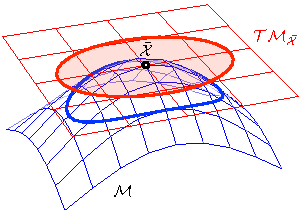
\includegraphics[width=0.6\columnwidth]{figures/covariance.pdf}
    \caption{Uncertainty around an element $\bar{\cX}$ on the manifold $\cM$ can be expressed as a covariance on the tangent vector space at the element (red).
    This lets us define a random variable on the tangent space that through perturbation with $\bar{\cX}$ induces the corresponding probability distribution on the manifold (blue).\\
    (Image source: \cite{SolaARobotics}; licensed under \href{https://creativecommons.org/licenses/by-nc-sa/4.0/}{CC BY-NC-SA 4.0})}
    \label{fig:uncertainty-on-manifold}
\end{figure}

We can represent a random variable on the manifold as a perturbation
\begin{equation}
  \cX = \bar{\cX} \oplus \vectau, \quad \vectau = \cX \ominus \bar{\cX},
\end{equation}
where $\bar{\cX} \in \cM$ is a nominal (noise-free) element, and $\vectau \in \bbR^m$ is a random variable in the tangent space $\cT\cM_{\bar{\cX}}$.
We can in this way define a PDF over $\vectau$ to induce a PDF on $\cX$.

Covariance matrices can be properly defined on $\cT\cM_{\bar{\cX}}$ with the expectation operator $\bbE[\cdot]$ as
\begin{equation}
  \matSigma_\cX = \bbE[\vectau \vectau\trans] = \bbE[(\cX \ominus \bar{\cX}) (\cX \ominus \bar{\cX})\trans] \in \bbR^{m \times m}.
\end{equation}
This lets us define the Gaussian PDF for the tangent space vector
\begin{equation}
  \vectau \sim \cN(\matr{0}, \matSigma_\cX),
\end{equation}
and the induced Gaussian PDF on the manifold (Figure~\ref{fig:uncertainty-on-manifold})
\begin{equation}
  \cX \sim \cN(\bar{\cX}, \matSigma_\cX).
\end{equation}

\begin{example}[frametitle=Drawing random poses from a Gaussian distribution]
Using the framework presented above, we can draw random poses from a distribution $\matT \sim \cN(\bar{\matT}, \matSigma_\matT)$ by perturbing the mean pose $\bar{\matT}$ with tangent vectors drawn from the distribution $\vecxi \sim \cN(\matr{0}, \matSigma_\matT)$, so that $\matT = \bar{\matT} \oplus \vecxi$.

{
  \centering
  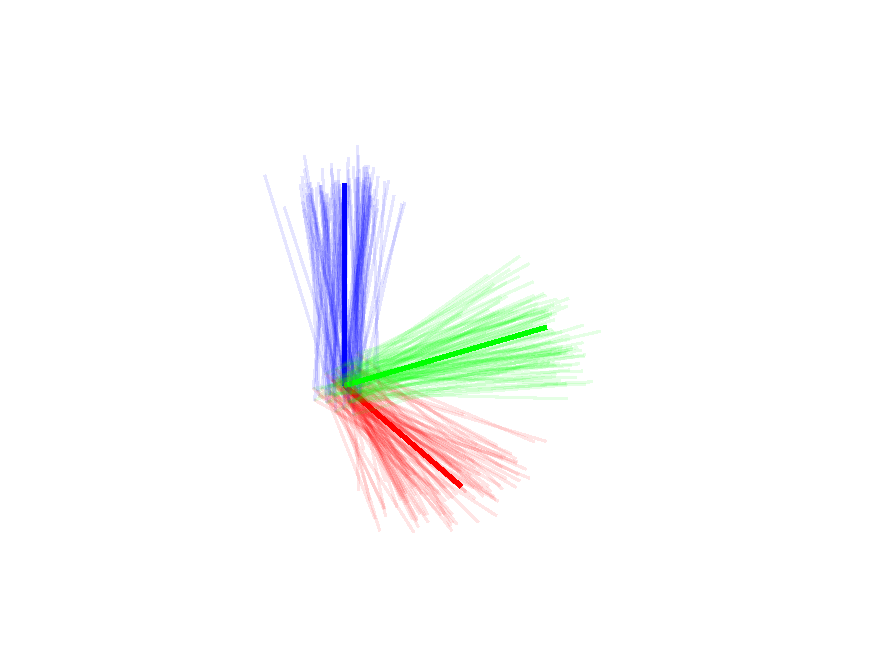
\includegraphics[width=0.75\columnwidth]{figures/draw-random-pose.pdf}
  \captionsetup{type=figure}
  \captionof{figure}{The mean pose $\bar{\matT}$ is shown in thick axes, while 50 poses drawn randomly from $\cN(\bar{\matT}, \matSigma_\matT)$ are shown in thin transparent axes.}
  \label{fig:draw-random-pose-example}
  \par
}

Figure~\ref{fig:draw-random-pose-example} shows the result of drawing 50 poses with $\bar{\matT} = \matI$ and

\begin{equation*}
  \matSigma_\matT =
  \begin{bmatrix}
    0.05 & & & & & \\
    & 0.05& & & & \\
    & & 0.05 & & & \\
    & & & 0.1 & & \\
    & & & & 0.1 & \\
    & & & & & 0.2 \\
  \end{bmatrix}.
\end{equation*}
\end{example}

It has been demonstrated that representing uncertainties on the manifold in this way captures the underlying distribution in stochastic kinematic models more accurately and more precisely, compared to representing uncertainties over position and orientation angles directly \cite{Long2012TheCoordinates}.

\begin{example}[frametitle=The banana distribution is Gaussian]
We will now demonstrate how a Gaussian PDF on the manifold lets us represent correlations between translation and orientation in a natural way with an experiment inspired from \cite{Long2012TheCoordinates}.

Consider an uncertain movement in the plane from the starting pose shown in black in Figure~\ref{fig:banana-distribution-example}.
Let the uncertain movement of 4 unit steps along the $x$-axis be represented by the stochastic 2D pose $\matT \in \SE(2)$, where $\matT \sim \cN(\bar{\matT}, \matSigma_\matT)$, and the uncertainty in translation along the $y$-axis and orientation are correlated:
\begin{equation*}
  \matSigma_\matT =
  \begin{bmatrix}
    0.1 & 0.0 & 0.0 \\
    0.0 & 2.0 & 0.4 \\
    0.0 & 0.4 & 0.1
  \end{bmatrix}.
\end{equation*}
We can visualise this distribution by transforming ellipsoids corresponding to constant probabilities to the plane by using the exponential map.
Figure~\ref{fig:banana-distribution-example} shows the probability contours corresponding to $75\%$ and $99\%$ in green, together with 100 randomly drawn poses from the same distribution.
Notice the distinct banana shape of the distribution in the plane, and how it fits with the clear correlation between position and orientation in the random pose samples.

{
  \centering
  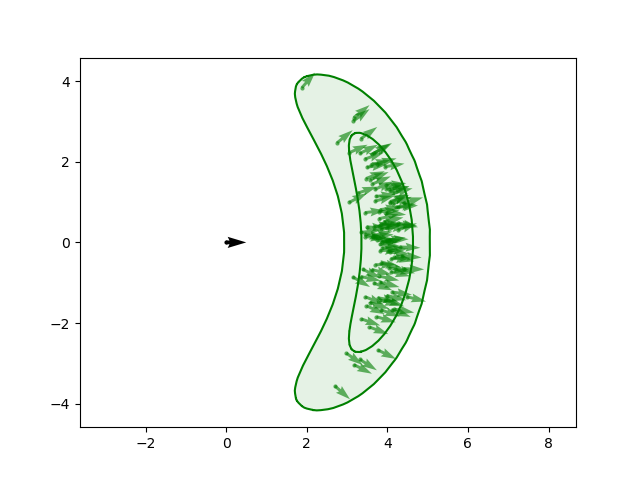
\includegraphics[width=0.75\columnwidth]{figures/banana-distribution.png}
  \captionsetup{type=figure}
  \captionof{figure}{The starting pose is shown as a black arrow, and the distribution representing the uncertain movement is visualised as filled green contours corresponding to $75\%$ and $99\%$ probabilities.
  100 pose samples drawn from the distribution are shown as green arrows.
  }
  \label{fig:banana-distribution-example}
  \par
}
\end{example}

\section{Propagation of uncertainty}
Let $f: \bbR^m \to \bbR^n$ be a function that takes the random variable $\vecx \in \bbR^m$ as input and produces the random variable $\vecy = f(\vecx) \in \bbR^n$ as output.
We will assume that $\vecx \sim \cN(\bar{\vecx}, \matSigma_\vecx)$.

Computing the uncertainty of the output $\vecy$ based on the effect of the uncertainties in the input $\vecx$ is sometimes called \emph{propagation of uncertainty}.
This is useful when we need to know the uncertainty in transformed variables, such as the uncertainty of poses in different coordinate frames, and the uncertainty in pixel position based on the uncertainty of a projected 3D point.

When $f(\vecx)$ is a linear function $\vecy = f(\vecx) = \matA\vecx + \vecb$, we can compute the probability distribution of $\vecy$ exactly.
Since the expectation operator is linear, we can compute the mean of $\vecy$ from the definition in \eqref{eq:mean-def} as
\begin{equation} \label{eq:linear-mean}
  \bar{\vecy} = \bbE[\vecy] = \bbE[\matA \vecx + \vecb] = \matA \bbE[\vecx] + \vecb = \matA \bar{\vecx} + \vecb = f(\bar{\vecx}).
\end{equation}
The covariance matrix of $\vecy$ is developed similarly from the definition in \eqref{eq:cov-def} by
\begin{subequations}\label{eq:linear-cov}
\begin{align}
  \matSigma_\vecy &= \bbE[(\vecy - \bar{\vecy}) (\vecy - \bar{\vecy})\trans]\\
  &= \bbE \left[  \left( (\matA \vecx + \vecb) - (\matA \bar{\vecx} + \vecb) \right) \left( (\matA \vecx + \vecb) - (\matA \bar{\vecx} + \vecb) \right)\trans \right]\\
  &= \bbE \left[ (\matA(\vecx - \bar{\vecx})) (\matA(\vecx - \bar{\vecx}))\trans \right]\\
  &= \bbE \left[ \matA(\vecx - \bar{\vecx}) (\vecx - \bar{\vecx})\trans \matA\trans \right]\\
  &= \matA \bbE\left[ (\vecx - \bar{\vecx}) (\vecx - \bar{\vecx})\trans \right] \matA\trans\\
  &= \matA \matSigma_\vecx \matA\trans.
\end{align}
\end{subequations}
The resulting probability distribution for $\vecy$ when $\vecy = f(\vecx)$ is linear is therefore given by
\begin{equation} \label{eq:linear-uncertainty-propagation}
  \vecy \sim \cN(f(\bar{\vecx}), \matA \matSigma_\vecx \matA\trans).
\end{equation}

\begin{example}[frametitle=Transforming random points with deterministic poses]
We are given the random 3D point $\vecx^c \sim \cN(\bar{\vecx}^c, \matSigma_{\vecx^c})$ in the camera frame $\cF_c$, and the \emph{deterministic} pose $\matT_{wc}$ of the camera frame relative to the world frame $\cF_w$.

Since $\vecx^w = \matT_{wc} \cdot \vecx^c = \matR_{wc}\vecx^c + \vect^w_{wc}$ is a linear function in $\vecx^c$, we can apply \eqref{eq:linear-uncertainty-propagation} to compute the exact distribution of the point in the world frame as
\begin{equation}
  \vecx^w \sim \cN(\matR_{wc}\bar{\vecx}^c + \vect^w_{wc}, \; \matR_{wc} \matSigma_{\vecx^c} \matR_{wc}\trans).
\end{equation}
\end{example}

For a random Lie group variable, $\cX \sim \cN(\bar{\cX}, \matSigma_\cX)$, since global and local perturbations are related linearly by the adjoint matrix \eqref{eq:adjoint-matrix}, we can transform the covariance matrices exactly between frames according to
\begin{equation}
  \prescript{\cE}{}{\matSigma}_\cX = \mAd_\cX \prescript{\cX}{}{\matSigma}_\cX {\mAd_\cX}\trans.
\end{equation}
This allows us to express the local distribution of $\cX$ exactly in the global frame.

For a \emph{nonlinear} function $g: \bbR^m \to \bbR^n$, where the random variable $\vecy$ is now given by $\vecy = g(\vecx)$, we will in general not get an exact Gaussian distribution over $\vecy$ when propagating the uncertainty of $\vecx$.
We can instead assume that $g(\vecx)$ is approximately linear around the mean of $\vecx$, so that we can use the propagation procedure above with the linear approximation.

We can linearise $g(\vecx)$ with a first order Taylor expansion \eqref{eq:linear-approximation} at the mean $\bar{\vecx}$ to get the linear form
\begin{equation} \label{eq:g-linearised}
  g(\vecx) = g(\bar{\vecx}  + (\vecx - \bar{\vecx})) \approx g(\bar{\vecx}) +  \jac{\vecy}{\bar{\vecx}}(\vecx - \bar{\vecx}),
\end{equation}
where the Jacobian is defined as
\begin{equation} \label{eq:noise-linearisation}
  \jac{\vecy}{\bar{\vecx}} \triangleq \dpar{g(\vecx)}{\vecx} \Bigr|_{\vecx = \bar{\vecx}}.
\end{equation}
Since $\bbE[\vecx - \bar{\vecx}] = \matr{0}$, developing the mean of \eqref{eq:g-linearised} according to \eqref{eq:linear-mean} gives us
\begin{equation}
  \bar{\vecy} \approx g(\bar{\vecx}).
\end{equation}
Developing the covariance matrix of \eqref{eq:g-linearised} according to \eqref{eq:linear-cov} results in
\begin{equation}
  \matSigma_\vecy \approx \jac{\vecy}{\bar{\vecx}}  \matSigma_\vecx \jac{\vecy}{\bar{\vecx}}\trans.
\end{equation}

We can therefore propagate the uncertainty through the nonlinear function $g(\vecx)$ by approximating it locally as a linear function $g(\bar{\vecx}) +  \jac{\vecy}{\bar{\vecx}}(\vecx - \bar{\vecx})$ to get the approximate PDF for $\vecy = g(\vecx)$ as
\begin{equation}
  \vecy \sim \cN(g(\bar{\vecx}), \jac{\vecy}{\bar{\vecx}}  \matSigma_\vecx \jac{\vecy}{\bar{\vecx}}\trans).
\end{equation}

It is also possible to perform uncertainty propagation using higher order approximations \cite{barfoot2017state}.

\begin{example}[frametitle=Uncertainty in backprojection] \label{ex:uncertainty-backrpojection}
Given a calibrated camera with intrinsic matrix
\begin{equation}
  \matK =
    \begin{bmatrix}
    f_u & 0 & c_u\\
    0 & f_v & c_v\\
    0 & 0 & 1
  \end{bmatrix},
\end{equation}
we can use the inverse perspective camera model,
\begin{equation}
  \vecx^c = \pi^{-1}(\vecu, z) = z \matK^{-1}
  \breve{\vecu}
  = z
  \begin{bmatrix}
   \frac{u - c_u}{f_u}\\[1em]
   \frac{v - c_v}{f_v}\\[1em]
    1
  \end{bmatrix},
\end{equation}
to compute the 3D point $\vecx^c$ in the camera frame that corresponds to a pixel $\vecu$ with depth $z$.
Given the pose $\matT_{wc}$ of the camera relative to the world frame, we get the corresponding world point from $\vecx^w = \matT_{wc} \cdot \vecx^c$.
This gives us the model
\begin{equation}
  \vecx^w = f(\matT_{wc}, \vecu, z) = \matT_{wc} \cdot \pi^{-1}(\vecu, z).
\end{equation}

We are given the parameters for the model as random variables
\begin{align}
  \matT_{wc} &\sim \cN(\bar{\matT}_{wc}, \matSigma_{\matT_{wc}})\\
  \vecu &\sim \cN(\bar{\vecu}, \matSigma_{\vecu})\\
  z &\sim \cN(\bar{z}, \sigma^2_z).
\end{align}

We can approximate the distribution for the backprojected point as
\begin{align}
  \bar{\vecx}^w &= f(\bar{\matT}_{wc}, \bar{\vecu}, \bar{z}) \label{eq:est_x}\\
  \matSigma_{\vecx^w} &= \jac{f}{\bar{\matT}_{wc}} \matSigma_{\matT_{wc}} {\jac{f}{\bar{\matT}_{wc}}}\trans +
  \jac{f}{\bar{\vecu}} \matSigma_{\vecu} \jac{f}{\bar{\vecu}}\trans +
  \jac{f}{\bar{z}} \sigma^2_z {\jac{f}{\bar{z}}}\trans. \label{eq:est_S}
\end{align}
Using the Jacobian blocks from section \ref{sec:Jacobians-SE3}, we get the Jacobians
\begin{align}
  \jac{f}{\bar{\matT}_{wc}} &= \jac{\bar{\matT}_{wc} \cdot \pi^{-1}}{\bar{\matT}_{wc}} = \jac{\bar{\matT}_{wc} \cdot \vecx^c}{\bar{\matT}_{wc}} = 
  \begin{bmatrix}
    \bar{\matR}_{wc} & -\bar{\matR}_{wc} \; [\vecx^c]_\times
  \end{bmatrix}\\[1em]
  \jac{f}{\bar{\vecu}} &= \jac{\bar{\matT}_{wc} \cdot \pi^{-1}}{\pi^{-1}} \jac{\pi^{-1}}{\bar{\vecu}} = \bar{\matR}_{wc}
    \begin{bmatrix}
    \frac{\bar{z}}{f_u} & 0\\
    0 & \frac{\bar{z}}{f_v}\\
    0 & 0
  \end{bmatrix}\\[1em]
  \jac{f}{\bar{z}} &= \jac{\bar{\matT}_{wc} \cdot \pi^{-1}}{\pi^{-1}} \jac{\pi^{-1}}{\bar{z}} = \bar{\matR}_{wc} \; \matK^{-1} \breve{\bar{\vecu}},
\end{align}
which allows us to compute the approximation $\vecx^w \sim \cN(\bar{\vecx}^w, \matSigma_{\vecx^w})$.
\end{example}

\section{Propagating uncertainty with Lie operations}
We will here (temporarily very briefly) present the main results from \cite{Mangelson2020CharacterizingAlgebra}, which lets us propagate uncertainty through important operations on Lie elements by also taking correlations into account.
The original paper is based on left perturbations, so we will here present the corresponding results for right perturbations.
See Appendix~\ref{ch:app-prop-lie-operations} for details.

\subsection{The inverse operation}
Given the distribution $\cX_{ij} \sim \cN(\bar{\cX}_{ij}, \matSigma_{\cX_{ij}})$, the corresponding distribution of the inverse element $\cX_{ji} = \cX_{ij}^{-1}$ is given by $\cX_{ji} \sim \cN(\bar{\cX}_{ji}, \matSigma_{\cX_{ji}})$, where these are exactly given as
\begin{align}
    \bar{\cX}_{ji} & = \bar{\cX}_{ij}^{-1}\\
    \matSigma_{\cX_{ji}} &= \mAd_{\bar{\cX}_{ij}} \matSigma_{\cX_{ij}} \mAd_{\bar{\cX}_{ij}}\trans.
\end{align}

\subsection{The composition operation}
Given the joint distribution over $[\cX_{ij}, \cX_{jk}]$, the distribution over the composition $\cX_{ik} = \cX_{ij} \circ \cX_{jk}$ is given to first order by
\begin{align}
    \bar{\cX}_{ik} &= \bar{\cX}_{ij} \circ \bar{\cX}_{jk}\\
    \matSigma_{\cX_{ik}} &\approx 
    \mAd_{\bar{\cX}_{jk}^{-1}} \matSigma_{\cX_{ij}} \mAd_{\bar{\cX}_{jk}^{-1}}\trans \nonumber\\
    &+ \matSigma_{\cX_{jk}} \nonumber\\
    &+ \mAd_{\bar{\cX}_{jk}^{-1}} \matSigma_{\cX_{ij}, \cX_{jk}}\\
    &+ \matSigma_{\cX_{jk}, \cX_{ij}} \mAd_{\bar{\cX}_{jk}^{-1}}\trans \nonumber
\end{align}

\subsection{The relative composition}
Given the joint distribution over $[\cX_{ij}, \cX_{ik}]$, the distribution over the relative composition $\cX_{jk} = \cX_{ij}^{-1} \circ \cX_{ik}$ is given to first order by
\begin{align}
  \bar{\cX}_{jk} &= \bar{\cX}_{ij}^{-1} \circ \bar{\cX}_{ik}\\
  \matSigma_{\cX_{jk}} &\approx 
  \mAd_{\bar{\cX}_{jk}^{-1}} \matSigma_{\cX_{ij}} \mAd_{\bar{\cX}_{jk}^{-1}}\trans \nonumber\\
    &+ \matSigma_{\cX_{ik}} \nonumber\\
    &- \mAd_{\bar{\cX}_{jk}^{-1}} \matSigma_{\cX_{ij}, \cX_{ik}}\\
    &- \matSigma_{\cX_{ik}, \cX_{ij}} \mAd_{\bar{\cX}_{jk}^{-1}}\trans \nonumber
\end{align}

\chapter{Nonlinear state estimation} \label{ch:nls}
This chapter will introduce a powerful framework for nonlinear state estimation based on nonlinear least squares.
This includes a simple notation for expressing such problems, and a procedure for obtaining the MAP estimate and its uncertainty, given Gaussian measurement noise.
Most of this chapter is based on \cite{Dellaert2017, barfoot2017state}.

\section{Linear least squares}
Consider a set of $n$ \emph{linear} equations in $m$ unknowns $\vecx = [x_1, \ldots, x_m]\trans$
\begin{equation}
  e_i(\vecx) = 0, \quad i = 1, \ldots, n.
\end{equation}
We can combine these equations on vector form as
\begin{equation} \label{eq:ls-equations}
  e(\vecx) = 
  \begin{bmatrix}
    e_1(\vecx)\\
    \vdots\\
    e_n(\vecx)
  \end{bmatrix}
  = \matr{0},
\end{equation}
where $e: \bbR^m \to \bbR^n$.

When $n > m$, it is typically not possible to find an exact solution to \eqref{eq:ls-equations}.
We can instead seek a solution that minimises the sum of squares of the \emph{residuals} $e(\vecx)$,
\begin{equation}
  f(\vecx) = e(\vecx)\trans e(\vecx) = \norm{e(\vecx)}^2,
\end{equation}
where $f(\vecx)$ is often called the \emph{objective function}.
Since \eqref{eq:ls-equations} is linear, we can obtain an objective function on the form
\begin{equation} \label{eq:objective-form}
  f(\vecx) = \norm{e(\vecx)}^2 = \norm{\matA\vecx - \vecb}^2,
\end{equation}
which means that we want to find the vector $\vecx$ so that
\begin{equation} \label{eq:ls-min-residual}
  \vecx^\ast = \argmin_\vecx f(\vecx) = \argmin_\vecx \norm{\matA\vecx - \vecb}^2.
\end{equation}
This is called a \emph{linear least squares} problem.

A solution to \eqref{eq:ls-min-residual} is required to have zero gradient, so that
\begin{equation}
  \dpar{f(\vecx^\ast)}{\vecx^\ast} = 2 \matA\trans (\matA \vecx^\ast - \vecb) = \matr{0}.
\end{equation}
This results in \emph{the normal equations}
\begin{align}
  \matA\trans \matA \vecx^\ast &= \matA\trans \vecb \label{eq:ls-normal-equations}\\
  \vecx^\ast &= (\matA\trans \matA)^{-1} \matA\trans \vecb,
\end{align}
which can be solved with Cholesky- or QR factorisation\footnotemark.
\footnotetext{Equivalent to \texttt{x = A\textbackslash b} in Matlab.}

\section{Nonlinear least squares}
When the equations in $e(\vecx)$ are nonlinear, we have a \emph{nonlinear least squares} problem.
This results in a nonlinear objective function, which cannot be minimised directly using the normal equations in \eqref{eq:ls-normal-equations}.
We can instead assume that $f(\vecx)$ is approximately linear locally around the current estimate.
This lets us define a procedure starting from a suitable initial estimate, where we iteratively linearise the problem, solve the linearised problem using the normal equations, and update the estimate until convergence (Figure~\ref{fig:nls-procedure}).
\begin{figure}[htb]
    \centering
    \tikzstyle{process} = [rectangle, minimum width=9cm, minimum height=1cm, text centered]
\tikzstyle{arrow} = [ultra thick,->,>=stealth]

\begin{tikzpicture}[node distance=2cm]
\node (init) [process] {Choose a suitable initial estimate};
\node (linearise) [process, below of=init] {Linearise the problem at the current estimate};
\node (solve) [process, below of=linearise] {Find increment by solving the linearised problem};
\node (update) [process, below of=solve] {Update the estimate with the increment};

\draw [arrow] (init) -- (linearise);
\draw [arrow] (linearise) -- (solve);
\draw [arrow] (solve) -- (update);
\draw [arrow] (update.west) to [out=180,in=180] (linearise.west);
\end{tikzpicture}
    \caption{An iterative procedure for solving nonlinear least squares problems.}
    \label{fig:nls-procedure}
\end{figure}

The vector $\vecx$ is sometimes called a \emph{state variable}, which is typically used to the describe the physical state of an object or a system.
The pose of a camera in the world is an example of such a state variable.
Notice that we can concatenate several different state variables into the vector $\vecx$, 
\begin{equation}
  \vecx = 
  \begin{bmatrix}
    \vecx_1\\
    \vdots\\
    \vecx_p
  \end{bmatrix},
\end{equation}
and that the equations $e_i(\vecx)$ can be defined to operate on one or more these $p$ different state variables.
This lets us use the least squares framework to estimate several state variables at once, such as the poses of a whole set of cameras, instead of only one.

To conveniently represent state variables over both vector spaces and manifolds, we will broaden the definition of the plus and minus operators given in Section~\ref{sec:lie-plus-and-minus}.
First, the vectors $\vecx \in \bbR^m$ is a Lie group under addition, where the exponential map is the identity \cite{SolaARobotics}:
\begin{equation}
  \Exp: \bbR^m \to \bbR^m; \quad\quad \vecx = \Exp(\vecx).
\end{equation}
This means that $\vecx$ is its own tangent vector, and that $\oplus$ and $\ominus$ are in fact valid representations of vector addition and subtraction:
\begin{align}
  \vecx_a \oplus \vecx_b &= \vecx_a + \vecx_b\\
  \vecx_b \ominus \vecx_a &= \vecx_b - \vecx_a,
\end{align}
where $\vecx_a, \vecx_b \in \bbR^m$.

We can now define $\ubar{\cX}$ as the concatenation of state variables
\begin{equation} \label{eq:concatenated-states}
  \ubar{\cX} \triangleq
  \begin{Bmatrix}
    \cX_1\\
    \vdots\\
    \cX_p
  \end{Bmatrix}
  \in \cM,
\end{equation}
where $\cX_i \in \cM_i$ and $\cM = \{\cM_1, \ldots, \cM_p\}$ is the \emph{composite manifold}, which can cover both vector spaces, orientations, poses and other manifolds.
We define $\ubar{\vectau}$ to be the corresponding concatenation of tangent vectors
\begin{equation}
  \ubar{\vectau} \triangleq
  \begin{bmatrix}
    \vectau_1\\
    \vdots\\
    \vectau_p
  \end{bmatrix}
  \in \bbR^m,
\end{equation}
where $\vectau_i$ is in the tangent space of $\cM_i$.
This lets us define the plus and minus operators for the concatenated state variable $\ubar{\cX}$ as
\begin{align}
  \ubar{\cX} \oplus \ubar{\vectau} &\triangleq
  \begin{Bmatrix}
    \cX_1 \oplus \vectau_1\\
    \vdots\\
    \cX_p \oplus \vectau_p
  \end{Bmatrix} \in \cM\\[1em]
  \ubar{\cY} \ominus \ubar{\cX} &\triangleq
   \begin{bmatrix}
    \cY_1 \ominus \cX_1\\
    \vdots\\
    \cY_p \ominus \cX_p
  \end{bmatrix}\in \bbR^m.
\end{align}

If we define $\ubar{\cX}_i$ to be the concatenated set of state variables taken as input by the $i$-th nonlinear equation $e_i(\ubar{\cX}_i)$, we get the nonlinear objective function
\begin{equation} \label{eq:nonlinear-objective-function}
  f(\ubar{\cX}) = \norm{e(\ubar{\cX})}^2 = \sum^n_{i=1} \norm{e_i(\ubar{\cX}_i)}^2.
\end{equation}
We can linearise $e_i(\ubar{\cX}_i)$ around the current estimate $\ubar{\hat{\cX}}_i$ using a first order Taylor expansion \eqref{eq:lie-linearisation} as
\begin{equation}
  e_i(\ubar{\cX}_i) = e_i(\ubar{\hat{\cX}}_i \oplus \ubar{\vectau}_i) \approx e_i(\ubar{\hat{\cX}}_i) + \jac{e_i}{\ubar{\hat{\cX}}_i} \ubar{\vectau}_i,
\end{equation}
where $\ubar{\vectau}_i = \ubar{\cX}_i \ominus \ubar{\hat{\cX}}_i$.

Applying the linearised residual functions in \eqref{eq:nonlinear-objective-function} allows us linearise the objective function as
\begin{equation} \label{eq:linearised-objective-function}
\begin{split}
    f(\ubar{\cX}) = f(\ubar{\hat{\cX}} \oplus \ubar{\vectau}) &\approx \sum^n_{i=1} \norm{e_i(\ubar{\hat{\cX}}_i) + \jac{e_i}{\ubar{\hat{\cX}}_i} \ubar{\vectau}_i}^2\\
    &= \sum^n_{i=1} \norm{\jac{e_i}{\ubar{\hat{\cX}}_i} \ubar{\vectau}_i - (-e_i(\ubar{\hat{\cX}}_i))}^2\\
    &= \sum^n_{i=1} \norm{\matA_i \ubar{\vectau}_i - \vecb_i}^2\\
    &= \norm{\matA \ubar{\vectau} - \vecb}^2,
\end{split}
\end{equation}
where $\ubar{\vectau} = \ubar{\cX} \ominus \ubar{\hat{\cX}}$ is the \emph{state update vector}, the Jacobians $\matA_i = \jac{e_i}{\ubar{\hat{\cX}}_i}$ are submatrices of the Jacobian $\matA = \jac{f}{\ubar{\hat{\cX}}}$, and the errors $\vecb_i = -e_i(\ubar{\hat{\cX}}_i)$ are the subvectors of the errors $\vecb = -e(\ubar{\hat{\cX}})$.

Since the linearised objective function in \eqref{eq:linearised-objective-function} now describes a linear least squares problem, we can compute the state update vector $\ubar{\vectau}^\ast$ that minimises this function by solving the normal equations in \eqref{eq:ls-normal-equations}.
This leads to the well known Gauss-Newton algorithm, which is given i Algorithm~\ref{alg:gauss-newton}.

\begin{algorithm}[H] \label{alg:gauss-newton}
\SetAlgoLined
\DontPrintSemicolon
\KwData{An objective function $f(\ubar{\cX})$ and a good initial state estimate $\ubar{\hat{\cX}}^0$}
\KwResult{An estimate for the states $\ubar{\hat{\cX}}$}
 \;
 \For{$t = 0, 1, \ldots, t^{\text{max}}$}{
  $\matA, \vecb \leftarrow$ Linearise $f(\ubar{\cX})$ at $\ubar{\hat{\cX}}^t$\;
  $\ubar{\vectau} \leftarrow$ Solve the linearised problem $\matA\trans \matA \ubar{\vectau} = \matA\trans \vecb$\;
  $\ubar{\hat{\cX}}^{t+1} \leftarrow \ubar{\hat{\cX}}^t \oplus \ubar{\vectau}$\;
  \;
  \If{$f(\ubar{\hat{\cX}}^{t+1})$ is very small or $\ubar{\hat{\cX}}^{t+1} \approx \ubar{\hat{\cX}}^t$}{
   $\ubar{\hat{\cX}} \leftarrow \ubar{\hat{\cX}}^{t+1}$\;
   \Return \;
   }
 }
 \caption{The Gauss-Newton algorithm}
\end{algorithm}

\begin{example}[frametitle=Estimating the mean of a set of poses]
Given a set of poses $\{\matT_1, \ldots, \matT_n\}$, we define an estimate for the mean pose $\bar{\matT}$ as the pose that minimises
\begin{equation}
  f(\bar{\matT}) = \sum^n_{i=1} \norm{\matT_i \ominus \bar{\matT}}^2.
\end{equation}
Here, the state variable we wish to estimate is $\bar{\matT}$, and the equations we wish to minimise are
\begin{equation}
  e_i(\bar{\matT}) = \matT_i \ominus \bar{\matT},
\end{equation}
which correspond to the tangent vectors at $\bar{\matT}$, between $\bar{\matT}$ and each of the given poses $\matT_i$.
We need to solve this iteratively, since we want to minimise $f(\bar{\matT})$ at the correct tangent space.

We can linearise the residual functions using a first order Taylor expansion by
\begin{equation}
  e_i(\bar{\matT} \oplus \vecxi) \approx e_i(\bar{\matT}) + \jac{e_i}{\bar{\matT}} \vecxi.
\end{equation}
From \eqref{eq:jacobian-minus-x-SE3} we see that the Jacobian is given by
\begin{equation}
  \jac{e_i}{\bar{\matT}} = \jac{\matT_i \ominus \bar{\matT}}{\bar{\matT}} =  -\jac{}{l}^{-1}(\matT_i \ominus \bar{\matT}),
\end{equation}
where the inverse left Jacobian $\jac{}{l}^{-1}$ for $\SE(3)$ is given in \eqref{eq:jacobian-left-inverse-SE3}.

The linearised least squares problem is then given by
\begin{align} 
  \vecxi^\ast &= \argmin_{\vecxi} \sum^n_{i=1} \norm{\matA_i \vecxi - \vecb_i}^2 \label{eq:pose_mean_ls_sum}\\
  &= \argmin_{\vecxi} \norm{\matA \vecxi - \vecb}^2,
\end{align}
where
\begin{align}
  \matA_i &=  -\jac{}{l}^{-1}(\matT_i \ominus \bar{\matT}) \label{eq:pose-mean-A-lin}\\
  \vecb_i &= - \matT_i \ominus \bar{\matT} \label{eq:pose-mean-b-lin},
\end{align}
and
\begin{equation}
  \matA =  
  \begin{bmatrix}
    \matA_1\\
    \vdots\\
    \matA_n
  \end{bmatrix}
  \qquad
  \vecb =  
  \begin{bmatrix}
    \vecb_1\\
    \vdots\\
    \vecb_n
  \end{bmatrix}.
\end{equation}
This lets us solve the problem with Gauss-Newton, as shown in Algorithm~\ref{alg:mean-pose-gauss-newton}. 


\begin{algorithm}[H] \label{alg:mean-pose-gauss-newton}
\SetAlgoLined
\DontPrintSemicolon
\KwData{A set of poses $\{\matT_1, \ldots, \matT_n\}$}
\KwResult{An estimate of the mean pose $\bar{\matT}$}
 \;
 Initialise for example with $\bar{\matT}^0 \leftarrow \matT_1$\;
 \;
 \For{$t = 0, 1, \ldots, t^{\text{max}}$}{
  $\matA, \vecb \leftarrow$ Linearise at $\bar{\matT}^t$ according to \eqref{eq:pose-mean-A-lin} and \eqref{eq:pose-mean-b-lin}\;
  $\vecxi \leftarrow$ Solve the linearised problem $\matA\trans \matA \vecxi = \matA\trans \vecb$\;
  $\bar{\matT}^{t+1} \leftarrow \bar{\matT}^t \oplus \vecxi$\;
  \;
  \If{$||\bar{\matT}^t \ominus \bar{\matT}^{t+1}||^2 < \epsilon$}{
   $\bar{\matT} \leftarrow \bar{\matT}^{t+1}$\;
   \Return \;
   }
 }
 \caption{Estimating the mean pose with Gauss-Newton}
\end{algorithm}

When $\bar{\matT}$ is close to $\matT_i$, $-\matA_i$ is close to the identity $\matI$.
With the approximation $-\matA_i \approx \matI$, the least-squares problem in \eqref{eq:pose_mean_ls_sum} corresponds to finding the mean tangent vector $\matT_i \ominus \bar{\matT}$ in the tangent space of $\bar{\matT}$ as
\begin{equation}
  \vecxi^\ast = \frac{1}{n} \sum^n_{i=1} \matT_i \ominus \bar{\matT}.
\end{equation}
By updating the tangent space iteratively with the current hypothesis for $\bar{\matT}$, we get the simpler iterative procedure in Algorithm~\ref{alg:iterative-mean-pose}.


\begin{algorithm}[H] \label{alg:iterative-mean-pose}
\SetAlgoLined
\DontPrintSemicolon
\KwData{A set of poses ${\matT_1, \ldots, \matT_n}$}
\KwResult{An estimate of the mean pose $\bar{\matT}$}
 \;
 Initialise for example with $\bar{\matT}^0 \leftarrow \matT_1$\;
 \;
 \For{$t = 0, 1, \ldots, t^{\text{max}}$}{
  Compute the mean tangent vector in the tangent space at $\bar{\matT}^t$\;
  $\bar{\vecxi} = \frac{1}{n} \sum^n_{i=1} \matT_i \ominus \bar{\matT}^t$\;
 \;
  Update the hypothesis\;
  $\bar{\matT}^{t+1} \leftarrow \bar{\matT}^t \oplus \bar{\vecxi}$\;
  \;
  \If{$||\bar{\matT}^t \ominus \bar{\matT}^{t+1}||^2 < \epsilon$}{
   $\bar{\matT} \leftarrow \bar{\matT}^{t+1}$\;
   \Return \;
   }
 }
 \caption{Iterative estimation of mean pose}
\end{algorithm}

{
  \centering
  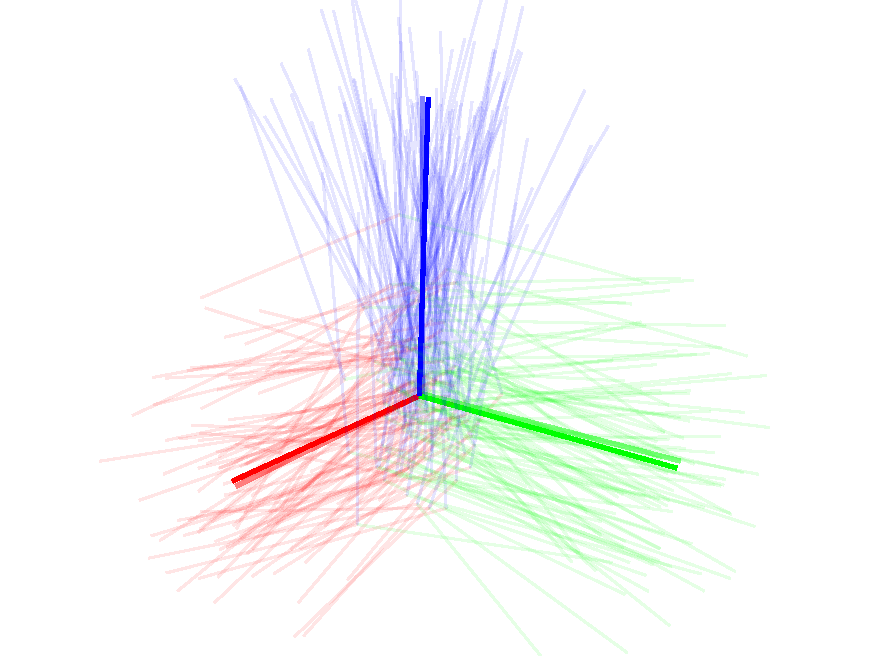
\includegraphics[width=0.75\columnwidth]{figures/mean-pose-example.pdf}
  \captionsetup{type=figure}
  \captionof{figure}{100 randomly drawn poses are shown in thin transparent axes, while the true mean is shown in thick transparent axes. The mean estimated using Algorithm~\ref{alg:iterative-mean-pose} is shown in thick solid axes.}
  \label{fig:mean-pose-example}
  \par
}
The procedure in Algorithm~\ref{alg:iterative-mean-pose} is shown to converge at least linearly if the initial estimate is close enough to the solution \cite{Arsigny2006Bi-invariant.}.
We can also apply the hybrid representation in Section~\ref{sec:hybrid-representation} to simplify the procedure even further.
Figure~\ref{fig:mean-pose-example} shows an example of estimating the mean of a set of randomly drawn poses.
\end{example}

The Gauss-Newton algorithm can approach quadratic convergence rate in some situations.
This is because it computes step lengths by approximating the Hessian of the objective function $f(\ubar{\cX})$ at $\ubar{\hat{\cX}}$ as
\begin{equation}
\begin{split}
  \frac{\partial^2 f(\ubar{\hat{\cX}})}{\partial \ubar{\hat{\cX}} \partial \ubar{\hat{\cX}}\trans} &= \left( \dpar{e(\ubar{\hat{\cX}})}{\ubar{\hat{\cX}}} \right)\trans \left( \dpar{e(\ubar{\hat{\cX}})}{\ubar{\hat{\cX}}} \right) +
  \sum_{i=1}^n e_i(\ubar{\hat{\cX}}_i) \frac{\partial^2 e_i(\ubar{\hat{\cX}}_i)}{\partial \ubar{\hat{\cX}}_i \partial \ubar{\hat{\cX}}_i\trans}\\[1em]
  &= \matA\trans \matA + \matQ \approx \matA\trans \matA.
\end{split}
\end{equation}
This approximation is good if we are near the solution, and the objective function is nearly quadratic.
If the quadratic fit is poor, Gauss-Newton might still estimate decent update directions, but the step lengths may be bad.
This may lead to new estimates that are further away from the minimum, and subsequent divergence.

Since the Gauss-Newton algorithm is not guaranteed to converge because of the Hessian approximation, it is sometimes beneficial to modify the algorithm to be more conservative towards robustness, rather than speed.
One solution is to update the estimate with only a fraction $\alpha$ of the update vector
\begin{equation}
  \ubar{\hat{\cX}}^{t+1} \leftarrow \ubar{\hat{\cX}}^t \oplus \alpha \ubar{\vectau},
\end{equation}
We can find good values for $\alpha$ by performing a \emph{line search} \cite{barfoot2017state}.

Another solution is to apply a \emph{trust region method}, which controls in which region one is willing to trust the quadratic Hessian approximation made by Gauss-Newton.
The \emph{Levenberg-Marquardt} algorithm is an example of such a method, where the normal equations \eqref{eq:ls-normal-equations} are modified by adding a non-negative constant to the diagonal
\begin{equation}
  \left( \matA\trans \matA + \lambda \diag(\matA\trans \matA) \right)\ubar{\vectau} = \matA\trans \vecb.
\end{equation}
When $\lambda = 0$ we obtain Gauss-Newton, while larger $\lambda$ causes larger steps in the steepest descent direction when the gradient is small, and more cautious steps when the gradient is large.
The complete Levenberg-Marquardt method is given in Algorithm~\ref{alg:levenberg-marquardt}.


\begin{algorithm}[H] \label{alg:levenberg-marquardt}
\SetAlgoLined
\DontPrintSemicolon
\KwData{An objective function $f(\ubar{\cX})$ and a good initial state estimate $\ubar{\hat{\cX}}^0$}
\KwResult{An estimate for the states $\ubar{\hat{\cX}}$}
 \;
 $\lambda \leftarrow 10^{-4}$\;
 \;
 \For{$t = 0, 1, \ldots, t^{\text{max}}$}{
  $\matA, \vecb \leftarrow$ Linearise $f(\ubar{\cX})$ at $\ubar{\hat{\cX}}^t$\;
  $\ubar{\vectau} \leftarrow$ Solve the linearised problem $( \matA\trans \matA + \lambda \diag(\matA\trans \matA))\ubar{\vectau} = \matA\trans \vecb$\;
  \;
  \eIf{$f(\ubar{\hat{\cX}}^t \oplus \ubar{\vectau}) < f(\ubar{\hat{\cX}}^t)$}
  {
    Accept update, increase trust region\;
    $\ubar{\hat{\cX}}^{t+1} \leftarrow \ubar{\hat{\cX}}^t \oplus \ubar{\vectau}$\;
    $\lambda \leftarrow \lambda / 10$
  }
  {
    Reject update, reduce trust region\;
    $\ubar{\hat{\cX}}^{t+1} \leftarrow \ubar{\hat{\cX}}^t$\;
    $\lambda \leftarrow \lambda * 10$
  }
  
  \;
  \If{$f(\ubar{\hat{\cX}}^{t+1})$ is very small or $\ubar{\hat{\cX}}^{t+1} \approx \ubar{\hat{\cX}}^t$}{
   $\ubar{\hat{\cX}} \leftarrow \ubar{\hat{\cX}}^{t+1}$\;
   \Return \;
   }
 }
 \caption{The Levenberg-Marquardt algorithm}
\end{algorithm}

\begin{example}[frametitle=Range-based localisation] \label{ex:range-based-localisation}
This example is inspired by an example in \cite{Boyd2017IntroductionSquares}.

{
  \centering
  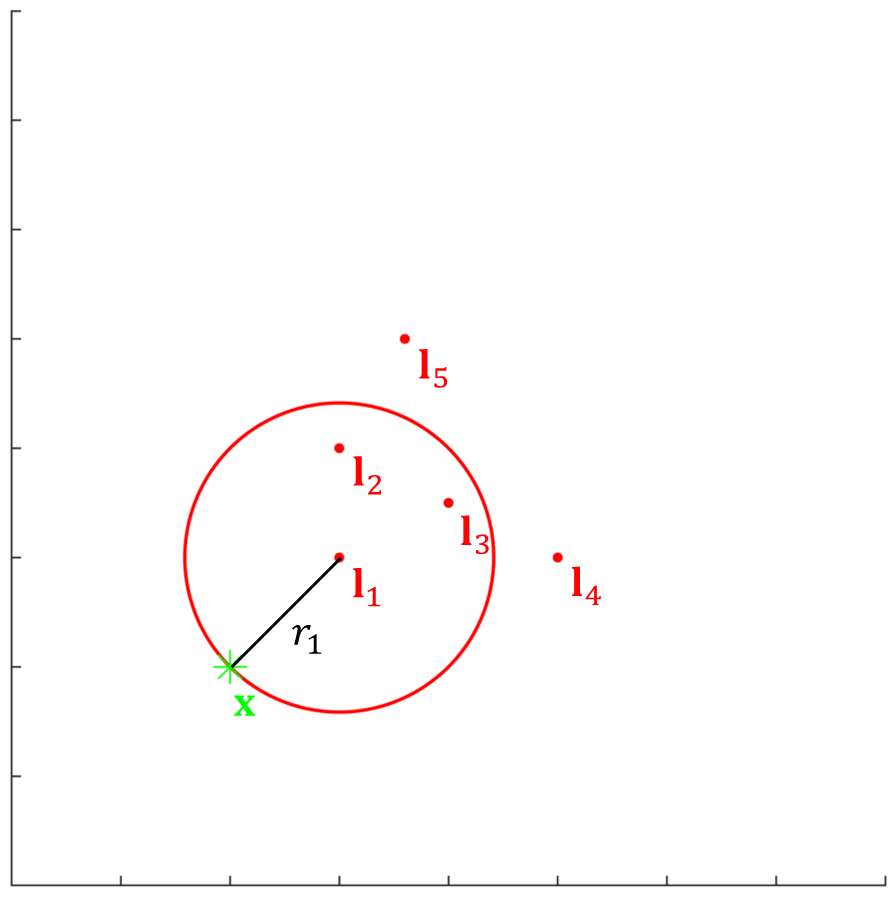
\includegraphics[height=7.5cm]{figures/range-localisation-intro.png}
  \captionsetup{type=figure}
  \captionof{figure}{Range-based localisation example.
  Our true position $\vecx$ is shown in green, while the known landmarks $\{\vecl_1, \ldots, \vecl_5\}$ are shown in red
  The range $r_1$ from $\vecl_1$ to our position is visualised as a red circle around the landmark.
  }
  \label{fig:range-localisation-intro}
  \par
}
We are given a set of ranges $\{r_1, \ldots, r_n\}$ to landmarks with known 2D positions $\{\vecl_1, \ldots, \vecl_n\}$, and we want to estimate our location $\vecx$ that minimises the errors between the predicted range $\norm{\vecx - \vecl_i}$ and the range measurement $r_i$,
\begin{equation}
  e_i(\vecx) = \norm{\vecx - \vecl_i} - r_i.
\end{equation}
This leads to the objective function
\begin{align}
  f(\vecx) &= \sum^n_{i=1} \norm{\norm{\vecx - \vecl_i} - r_i}^2\\
  &= \sum^n_{i=1} \left( \norm{\vecx - \vecl_i} - r_i \right)^2,
\end{align}
which we can solve as the nonlinear least squares problem
\begin{equation}
  \vecx^\ast = \argmin_\vecx \sum^n_{i=1} \left( \norm{\vecx - \vecl_i} - r_i \right)^2.
\end{equation}
We can linearise the error function at the current estimate $\hat{\vecx}$ as
\begin{equation} \label{eq:linearised-range-error}
  e_i(\hat{\vecx} + \delta\vecx) \approx e_i(\hat{\vecx}) + \jac{e_i}{\hat{\vecx}} \delta\vecx
\end{equation}
The Jacobian is given by (see Example~\ref{ex:jacobian-of-norm})
\begin{equation}
  \jac{e_i}{\hat{\vecx}} = \jac{\norm{\hat{\vecx} - \vecl_i}}{\hat{\vecx}} = \frac{(\hat{\vecx} - \vecl_i)\trans}{\norm{\hat{\vecx} - \vecl_i}}.
\end{equation}
Using \eqref{eq:linearised-objective-function}, we get the linearised least squares problem
\begin{align}
  \delta\vecx^\ast &= \argmin_{\delta\vecx} \sum^n_{i=1} \left( \matA_i \delta\vecx - b_i \right)^2\\
  &= \argmin_{\delta\vecx} \norm{\matA \delta\vecx - \vecb}^2,
\end{align}
where
\begin{align}
  \matA_i &= \jac{e_i}{\hat{\vecx}} = \frac{(\hat{\vecx} - \vecl_i)\trans}{\norm{\hat{\vecx} - \vecl_i}}\\
  b_i &= r_i - e_i(\hat{\vecx}) = r_i - \norm{\hat{\vecx} - \vecl_i}
\end{align}
and
\begin{equation}
  \matA =  
  \begin{bmatrix}
    \matA_1\\
    \vdots\\
    \matA_n
  \end{bmatrix}
  \qquad
  \vecb =  
  \begin{bmatrix}
    \vecb_1\\
    \vdots\\
    \vecb_n
  \end{bmatrix}.
\end{equation}
This lets us estimate $\hat{\vecx}$ using Gauss-Newton (Algorithm~\ref{alg:gauss-newton}) or Levenberg-Marquardt (Algorithm~\ref{alg:levenberg-marquardt}).

{
  \centering
  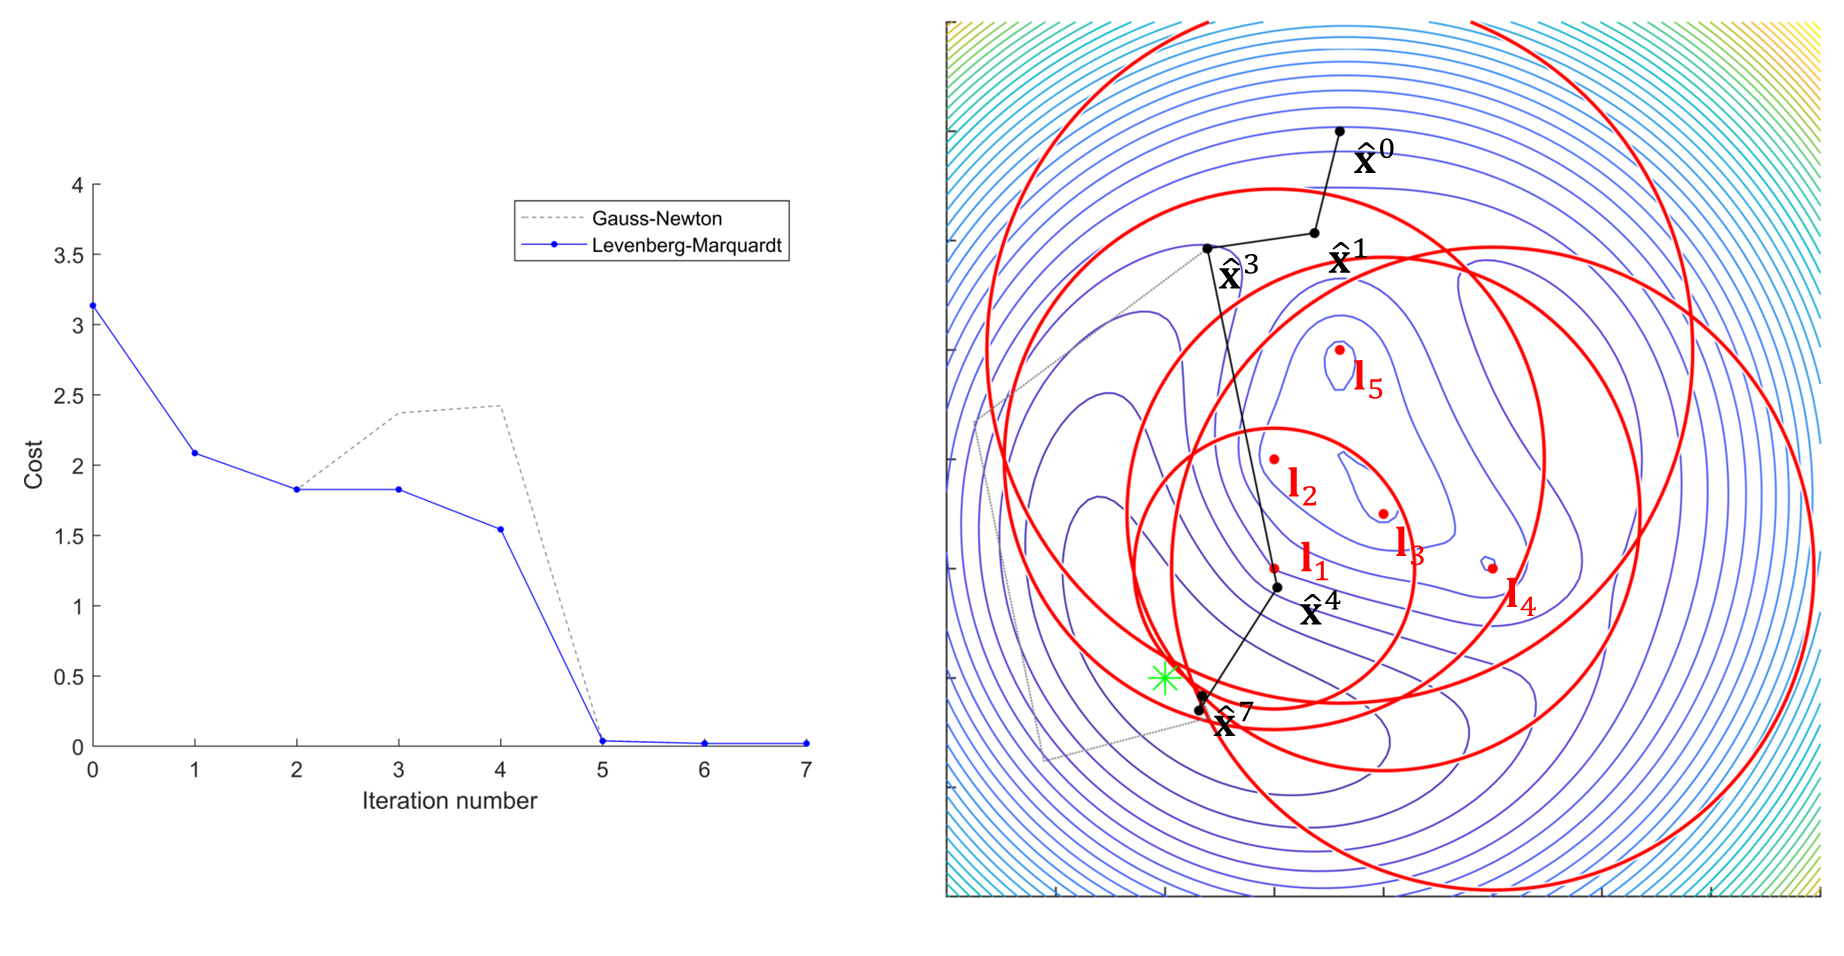
\includegraphics[width=1\columnwidth]{figures/range-localisation-LM-GN.png}
  \captionsetup{type=figure}
  \captionof{figure}{Example of applying Gauss-Newton and Levenberg-Marquardt to the range-based localisation problem.
  The range measurements are shown as red circles around their corresponding landmarks, and the coloured contours visualises the values of objective function at different locations.
  The iteration steps of the Levenberg-Marquardt algorithm are shown in black, while the steps of the Gauss-Newton algorithm are shown in grey.
  To the left we see how the error evolves with iterations for the two algorithms.
  We see that Gauss-Newton performs two steps that increases the error, while Levenberg-Marquardt always reduces the error in each step.
  }
  \label{fig:range-localisation-LM-GN}
  \par
}

Figure~\ref{fig:range-localisation-LM-GN} shows the difference between applying Gauss-Newton and Levenberg-Marquardt.
We see that both methods converge to a solution that minimises the objective function, but Gauss-Newton performs two steps that increases the error.
Figure~\ref{fig:range-localisation-LM-local-minimum} shows that  perturbing the initial estimate slightly results in convergence to an erroneous local minimum.

{
  \centering
  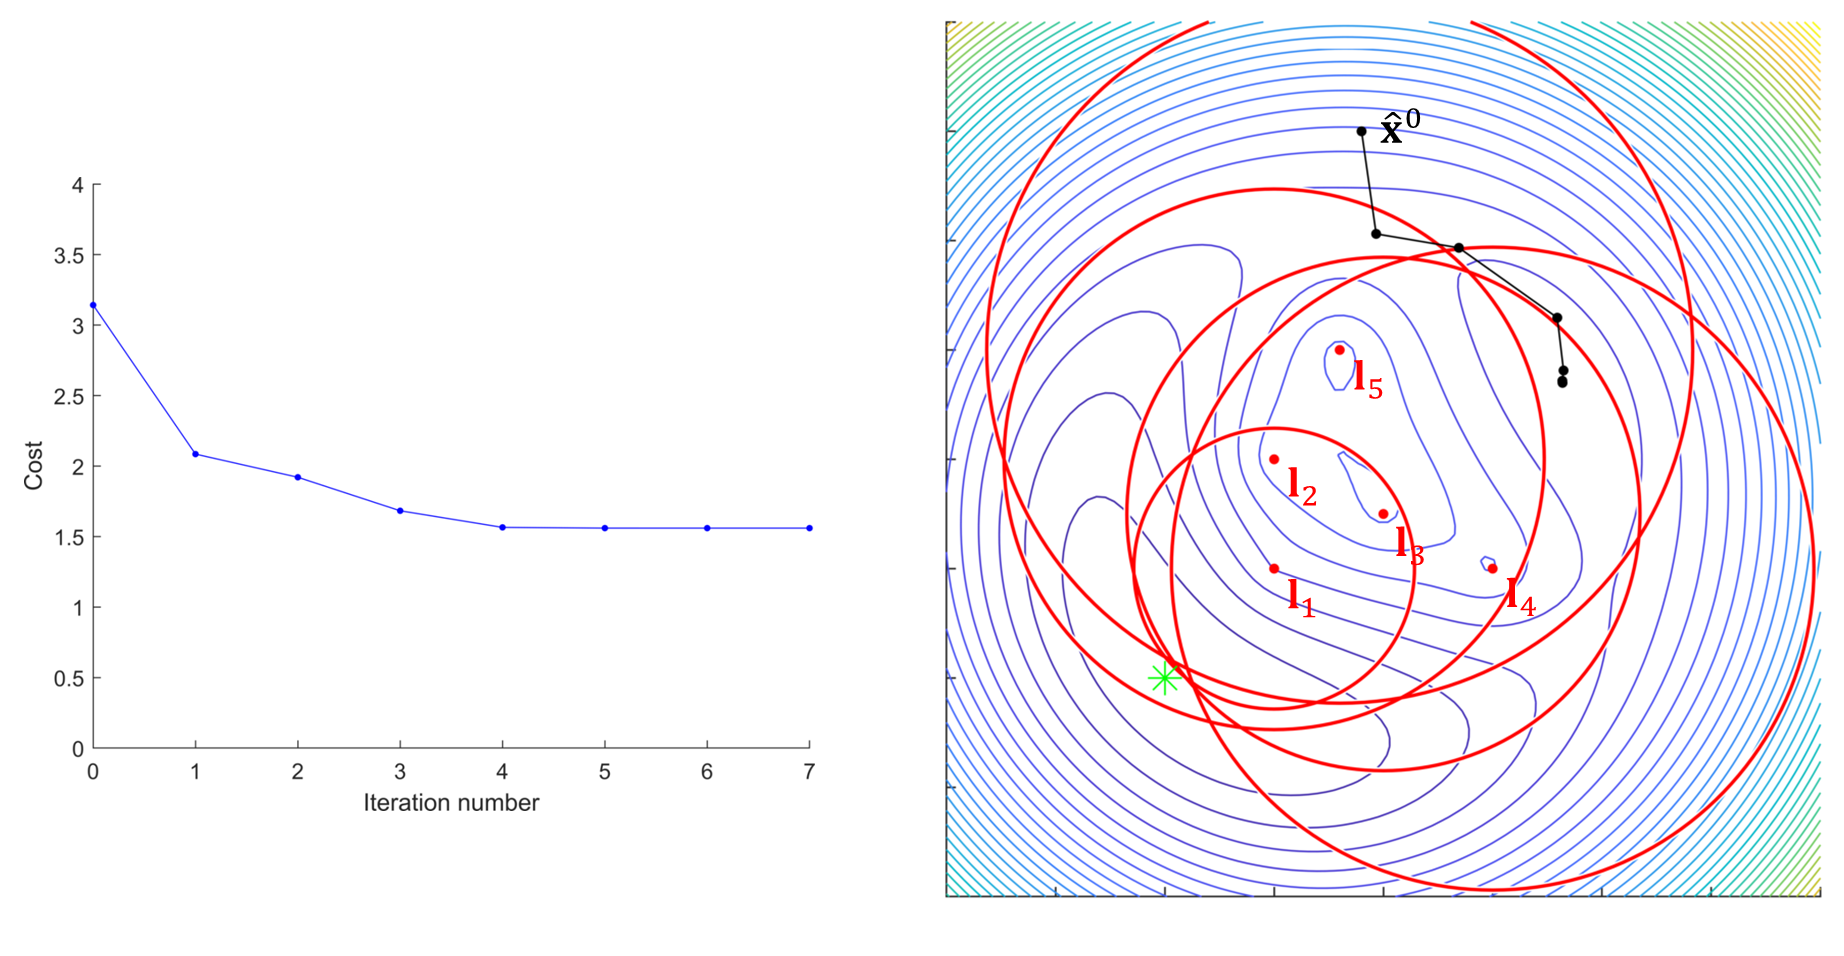
\includegraphics[width=1\columnwidth]{figures/range-localisation-LM-local-minimumpng.png}
  \captionsetup{type=figure}
  \captionof{figure}{The result when perturbing the initial estimate slightly to the right.
  In this situation, Levenberg-Marquardt converges to a local minima.
  Even though Levenberg-Marquardt is guaranteed to converge, it is not guaranteed to converge to the correct solution.
  }
  \label{fig:range-localisation-LM-local-minimum}
  \par
}

\end{example}

\section{Nonlinear MAP inference}
We will now turn to the problem of solving \emph{state estimation problems} based on noisy \emph{measurements}.
Assume that we want to estimate the unknown set of state variables $X$, and that we are given a set of sensor measurements $Z$ that depends upon the true state of $X$.
The most often used estimator for $X$ is the \emph{maximum a posteriori} (MAP) estimate, which maximises the \emph{posterior density} $p(X | Z)$ of the states $X$ given the measurements $Z$,
\begin{align} \label{eq:MAP}
    X^\text{MAP} &= \argmax_X p(X | Z).
\end{align}

Let the states $X$ be represented by the concatenation $\ubar{\cX}$ from \eqref{eq:concatenated-states}, and $Z$ be the set of measurement vectors $Z = \{\vecz_1, \ldots, \vecz_n \}$.
Let $\ubar{\cX}_i$ be the states involved in measurement $\vecz_i$.
Assuming that the measurements are corrupted by zero-mean Gaussian noise, we define the \emph{measurement model} as
\begin{equation}
  \vecz_i = h_i(\ubar{\cX}_i) + \eta_i, \qquad \eta_i \sim \cN(\matr{0}, \matSigma_i),
\end{equation}
where $h_i(\ubar{\cX}_i)$ is the \emph{measurement prediction function}.
We define the \emph{measurement error function} as the difference between the predicted measurement, given the states $\ubar{\cX}_i$, and the measurement $\vecz_i$,
\begin{equation}
  e_i(\ubar{\cX}_i) = h_i(\ubar{\cX}_i) - \vecz_i.
\end{equation}
It can be shown that the MAP estimate for the states $\ubar{\cX}$ given the measurements $Z$ is the solution to the nonlinear least squares problem,
\begin{equation} \label{eq:MAP-nls-problem}
  \ubar{\hat{\cX}}^{\text{MAP}} = \argmin_{\ubar{\cX}} \sum_{i=1}^n \norm{h_i(\ubar{\cX}_i) - \vecz_i}^2_{\matSigma_i},
\end{equation}
where
\begin{equation} \label{eq:mahalanobis-distance}
  \norm{\vece}^2_{\matSigma} \triangleq \vece\trans \matSigma^{-1} \vece = \left( \matSigma^{-1/2} \vece \right)\trans \left( \matSigma^{-1/2} \vece \right) = \norm{\matSigma^{-1/2} \vece}^2,
\end{equation}
is the squared Mahalanobis distance. 
We see from \eqref{eq:mahalanobis-distance} that the measurement errors are weighted according to the measurement uncertainties, so that good measurements will contribute more to the total error than uncertain measurements.
This is called \emph{covariance weighting}, and \eqref{eq:MAP-nls-problem} is therefore sometimes called a \emph{weighted nonlinear least squares} problem.

We can solve \eqref{eq:MAP-nls-problem} by first linearising the measurement prediction functions around the current estimate $\ubar{\hat{\cX}}$,
\begin{equation}
  h_i(\ubar{\cX}_i) = h_i(\ubar{\hat{\cX}}_i \oplus \ubar{\vectau}_i) \approx h_i(\ubar{\hat{\cX}}_i) + \jac{h_i}{\ubar{\hat{\cX}}_i} \ubar{\vectau}_i.
\end{equation}
This leads to the linearised measurement error function
\begin{equation}
  e_i(\ubar{\cX}_i) = e_i(\ubar{\hat{\cX}}_i \oplus \ubar{\vectau}_i) \approx h_i(\ubar{\hat{\cX}}_i) + \jac{h_i}{\ubar{\hat{\cX}}_i} \ubar{\vectau}_i - \vecz_i,
\end{equation}
and the linearised objective function 
\begin{equation} \label{eq:MAP-linearised-objective-function}
\begin{split}
    f(\ubar{\cX}) = f(\ubar{\hat{\cX}} \oplus \ubar{\vectau}) &= \sum^n_{i=1} \norm{e_i(\ubar{\hat{\cX}}_i \oplus \ubar{\vectau}_i)}^2_{\matSigma_i}\\
    &\approx \sum^n_{i=1} \norm{h_i(\ubar{\hat{\cX}}_i) + \jac{h_i}{\ubar{\hat{\cX}}_i} \ubar{\vectau}_i - \vecz_i}^2_{\matSigma_i}\\
    &= \sum^n_{i=1} \norm{\jac{h_i}{\ubar{\hat{\cX}}_i} \ubar{\vectau}_i - (\vecz_i - h_i(\ubar{\hat{\cX}}_i))}^2_{\matSigma_i}\\
    &= \sum^n_{i=1} \norm{\matSigma^{-1/2}_i \jac{h_i}{\ubar{\hat{\cX}}_i} \ubar{\vectau}_i - \matSigma^{-1/2}_i(\vecz_i - h_i(\ubar{\hat{\cX}}_i))}^2\\
    &= \sum^n_{i=1} \norm{\matA_i \ubar{\vectau}_i - \vecb_i}^2\\
    &= \norm{\matA \ubar{\vectau} - \vecb}^2.
\end{split}
\end{equation}
Notice that the weighted Jacobians
\begin{equation}
  \matA_i = \matSigma^{-1/2} \jac{h_i}{\ubar{\hat{\cX}}_i},
\end{equation}
and the weighted \emph{measurement prediction errors}
\begin{equation}
  \vecb_i =  \matSigma^{-1/2}(\vecz_i - h_i(\ubar{\hat{\cX}}_i)),
\end{equation}
have now undergone a form of \emph{whitening}, that eliminates the units of the measurements.

With the problem on linearised form, we can apply Gauss-Newton (Algorithm~\ref{alg:gauss-newton}) or Levenberg-Marquardt (Algorithm~\ref{alg:levenberg-marquardt}) to compute the MAP estimate $\ubar{\hat{\cX}}$, given a suitable initial estimate $\ubar{\hat{\cX}}^0$.
We can estimate the uncertainty in the MAP estimate by recognising that the Hessian of $f(\ubar{\cX})$ at the solution corresponds to the \emph{information matrix} of the estimate.
Using the Gauss-Newton approximation to the Hessian, we obtain a first order approximation of the true covariance, given by
\begin{equation}
  \matSigma_{\ubar{\hat{\cX}}} = \matLambda_{\ubar{\hat{\cX}}}^{-1} \approx (\matA_{\ubar{\hat{\cX}}}\trans \matA_{\ubar{\hat{\cX}}})^{-1}.
\end{equation}

\begin{example}[frametitle=Range-based localisation with measurement noise] \label{ex:range-based-localisation-noise}
We will revisit the range-based localisation example in Example~\ref{ex:range-based-localisation}, and see how we can apply the framework given in this section to naturally describe the state estimation problem, and solve it in the presence of measurement noise.

We are given a set of noisy range measurements $\{r_1, \ldots, r_n\}$ to landmarks with known 2D positions $\{\vecl_1, \ldots, \vecl_n\}$.
The measurement model is given by
\begin{equation}
  r_i = h_i(\vecx) + \eta_i, \qquad \eta \sim \cN(0, \sigma^2_i),
\end{equation}
where the measurement prediction function is
\begin{equation}
  h_i(\vecx) = \norm{\vecx - \vecl_i}.
\end{equation}
The measurement error is given by
\begin{equation}
  e_i(\vecx) = h_i(\vecx) - r_i = \norm{\vecx - \vecl_i} - r_i,
\end{equation}
leading to the covariance weighted nonlinear least squares problem
\begin{equation} \label{eq:range-MAP-weighted}
  \hat{\vecx}^{\text{MAP}} = \argmin_\vecx \sum^n_{i=1} \frac{1}{\sigma_i} \left( \norm{\vecx - \vecl_i} - r_i \right)^2
\end{equation}
By linearising the problem according to \eqref{eq:linearised-range-error} and \eqref{eq:MAP-linearised-objective-function}, we get the linearised least squares problem
\begin{align} \label{eq:range-MAP-linearised-problem}
  \delta\vecx^\ast &= \argmin_{\delta\vecx} \sum^n_{i=1} \left( \matA_i \delta\vecx - b_i \right)^2\\
  &= \argmin_{\delta\vecx} \norm{\matA \delta\vecx - \vecb}^2,
\end{align}
where
\begin{align}
  \matA_i &= \frac{1}{\sigma_i}\jac{e_i}{\hat{\vecx}} = \frac{1}{\sigma_i}\frac{(\hat{\vecx} - \vecl_i)\trans}{\norm{\hat{\vecx} - \vecl_i}}\\
  b_i &= \frac{1}{\sigma_i}(r_i - e_i(\hat{\vecx})) = \frac{1}{\sigma_i}(r_i - \norm{\hat{\vecx} - \vecl_i}).
\end{align}

Figure~\ref{fig:range-localisation-weighted} illustrates the difference between plain least squares and covariance weighted least squares.
In Figure~\ref{fig:range-localisation-covariance}, we see an illustration of the covariance estimated from the approximation to the Hessian, in the idealised case when all measurements are equal to the expected values.
 
{
  \centering
  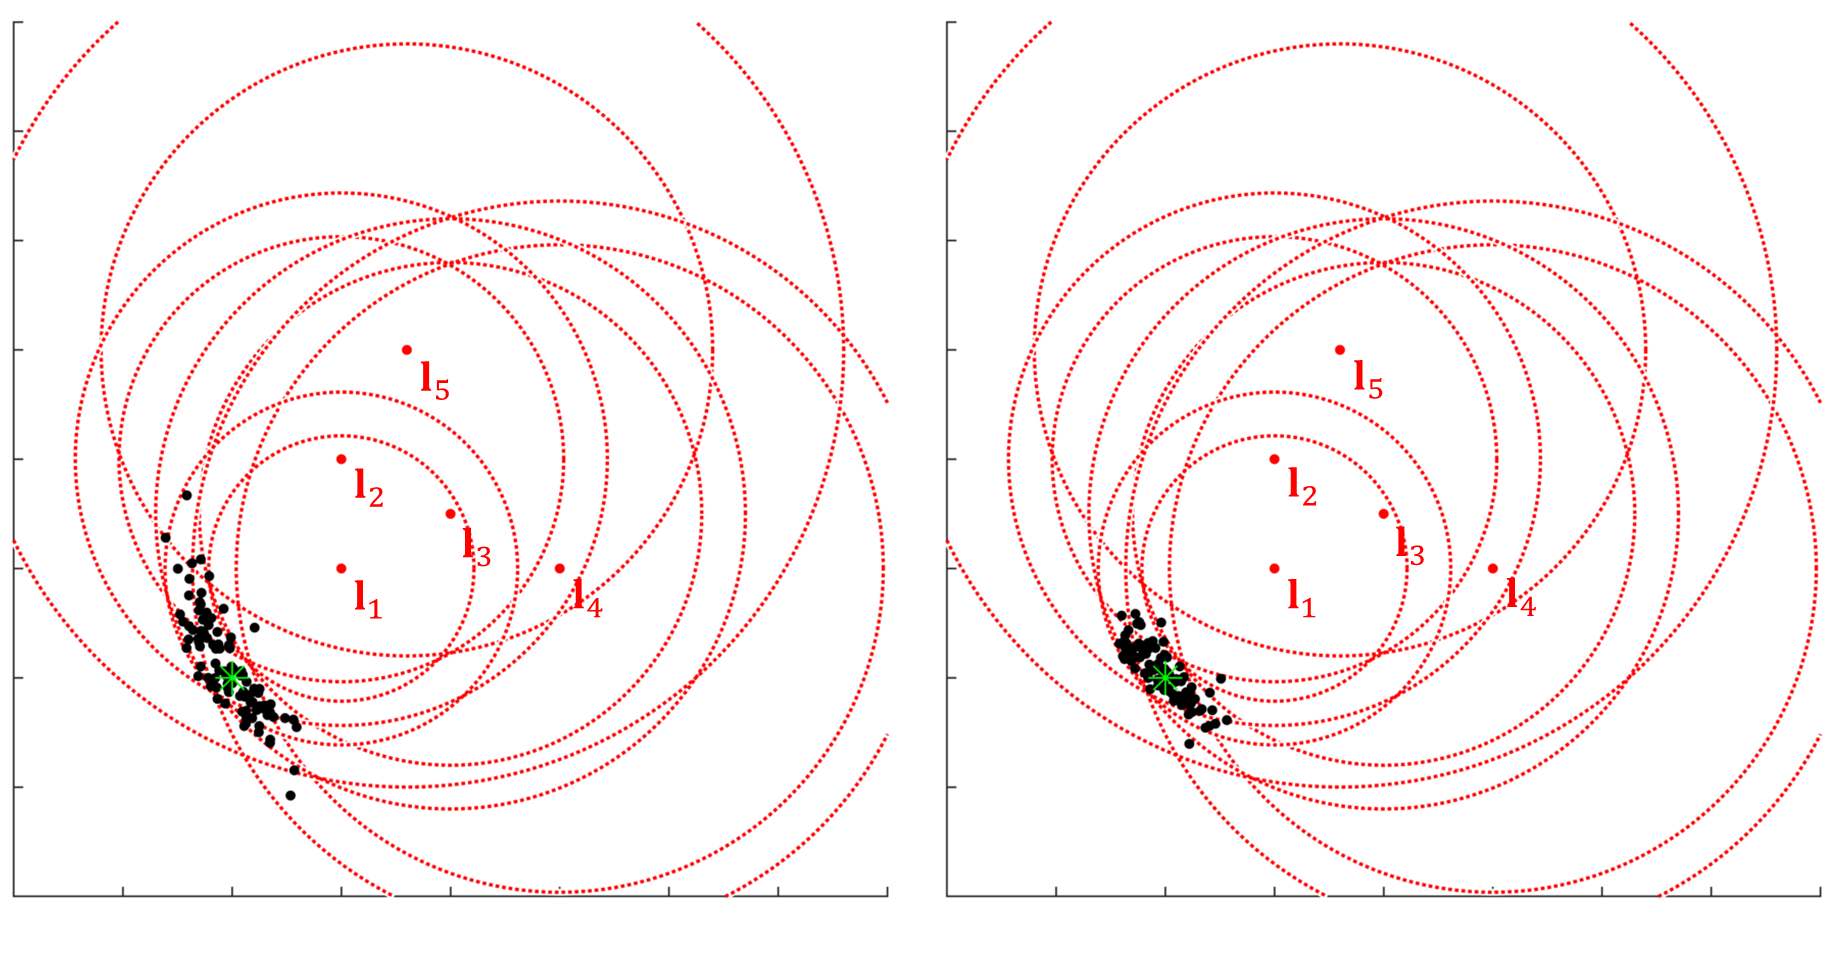
\includegraphics[width=\columnwidth]{figures/range-localisation-weighted.png}
  \captionsetup{type=figure}
  \captionof{figure}{The difference between not taking measurement noise into account, and performing covariance weighting.
  The noise on the range measurements is visualised as $\pm \sigma$ dotted circles around the landmarks.
  In this example, landmark $\vecl_5$ has triple the measurement noise compared to the other landmarks.
  Based on simulating 100 sets of measurements, we see on the left the result of estimating $\vecx$ without taking the noise into account.
  The uncertainty in the results are dominated by the uncertain measurements.
  On right, the same measurements have been used in the covariance weighted scheme in \eqref{eq:range-MAP-weighted}.
  We see that the influence of the noisy measurements have been significantly reduced.
  }
  \label{fig:range-localisation-weighted}
  \par
}

{
  \centering
  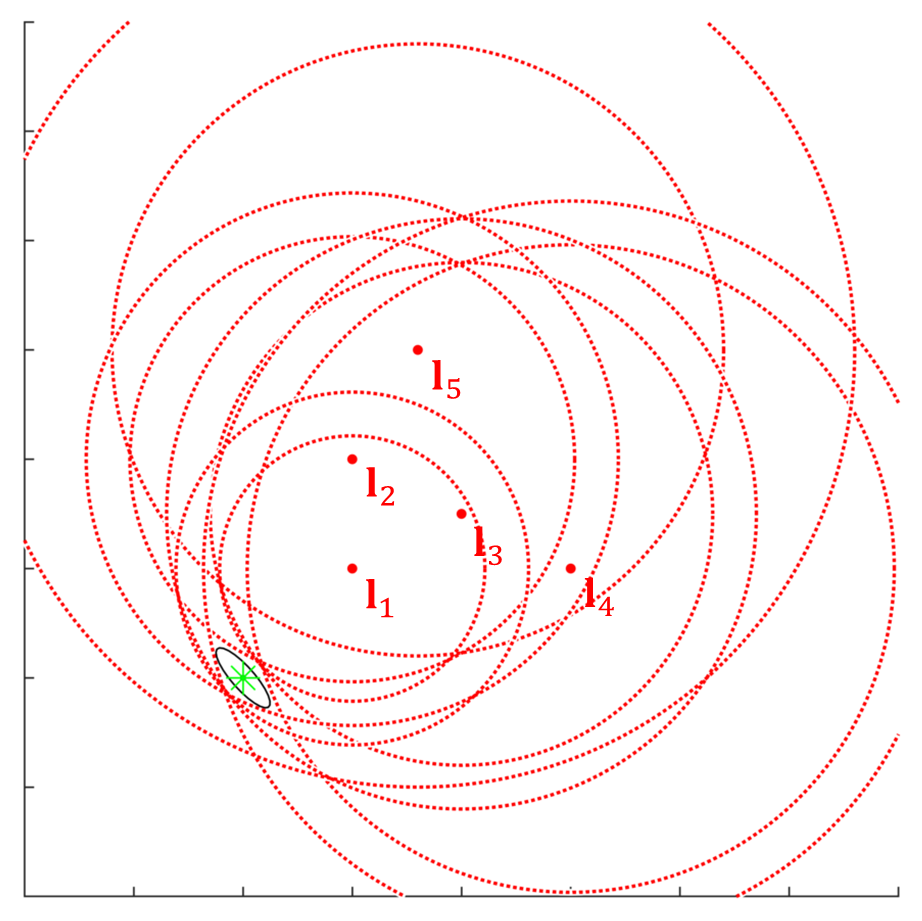
\includegraphics[height=7.5cm]{figures/range-localisation-covariance.png}
  \captionsetup{type=figure}
  \captionof{figure}{The covariance estimated from the approximation of the Hessian at the solution.
  Here, all measurements are set to the mean, to illustrate the connection between the uncertainty in the measurements, visualised as $\pm \sigma$ dotted circles around the landmarks, and the covariance of the estimate, shown as a black ellipse corresponding to the Mahalanobis distance at 1 standard deviation.
  }
  \label{fig:range-localisation-covariance}
  \par
}

\end{example}

The framework for MAP estimation described in this section makes it easy to express estimation problems where we want to find the best estimates for the states $\ubar{\cX}$, given a set of measurements $Z$.
By defining measurement prediction functions $h_i(\ubar{\cX}_i)$ for each measurement $\vecz_i$, and assuming Gaussian measurement noise, we can now obtain the MAP estimate and an estimate for its uncertainty.
This is done by linearising the measurement prediction function, using the tools from Chapter~\ref{ch:jacobians}, and applying the Gauss-Newton method from Algorithm~\ref{alg:gauss-newton} or the Levenberg-Marquardt method in Algorithm~\ref{alg:levenberg-marquardt}.

Notice that we have not assumed that all the measurements have the same type of measurement prediction function.
This means that we also can use this framework to put several different types of constraints on the state variables, such as priors on states, as well as measurements from different types of sensors.
We will in the next section see how we can apply this framework to estimate pose and structure from images.

\begin{example}[frametitle=Range-based localisation with prior]

{
  \centering
  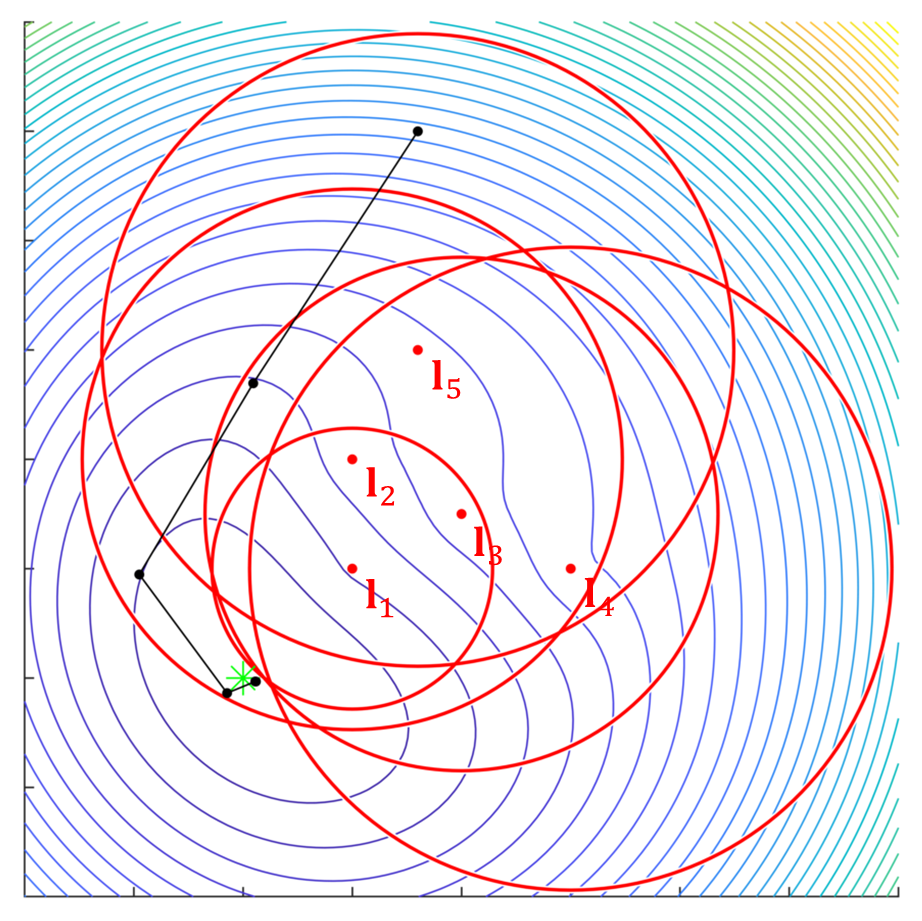
\includegraphics[height=7.5cm]{figures/range-localisation-prior.png}
  \captionsetup{type=figure}
  \captionof{figure}{The result of adding a prior to the problem in \eqref{eq:range-MAP-linearised-problem}.
  The expected value of the prior is set to the true state, and the standard deviation in both directions correspond to the measurement noise for the noisiest landmark $\vecl_5$.
  Compared to Figure~\ref{fig:range-localisation-LM-GN}, we see that the cost function is smoother, with a much better defined global minimium.
  The Gauss-Newton iterations shown in black traverses more directly towards the solution.
  }
  \label{fig:range-localisation-prior}
  \par
}

We can add a prior distribution $\cN(\bar{\vecx}_p, \matSigma_p)$ on our position in the problem in Example~\ref{ex:range-based-localisation-noise}, by adding another constraint on the state $\vecx$.

We can define the ``measurement model'' for the prior distribution as
\begin{equation}
  \matr{0} = h_p(\vecx) + \eta_p, \qquad \eta \sim \cN(\matr{0}, \matSigma_p),
\end{equation}
where the measurement prediction function simply is
\begin{equation}
  h_p(\vecx) = \vecx - \bar{\vecx}_p.
\end{equation}
Since $\jac{h_p}{\hat{\vecx}} = \matI$, we can add the prior constraint by adding the following Jacobian blocks and prediction errors to $\matA$ and $\vecb$ in \eqref{eq:range-MAP-linearised-problem}:
\begin{align}
  \matA_p &= \matSigma_p^{-1/2} \matI = \matSigma_p^{-1/2}\\
  \vecb_p &= \matSigma_p^{-1/2} (\matr{0} - (\vecx - \bar{\vecx}_p)) = \matSigma_p^{-1/2} (\bar{\vecx}_p - \vecx).
\end{align}
Figure~\ref{fig:range-localisation-prior} shows an example of adding a strict prior on $\vecx$. 

\end{example}

\chapter{Estimating pose and structure} \label{ch:estimating-pose-and-structure}
\begin{figure}[htb]
    \centering
    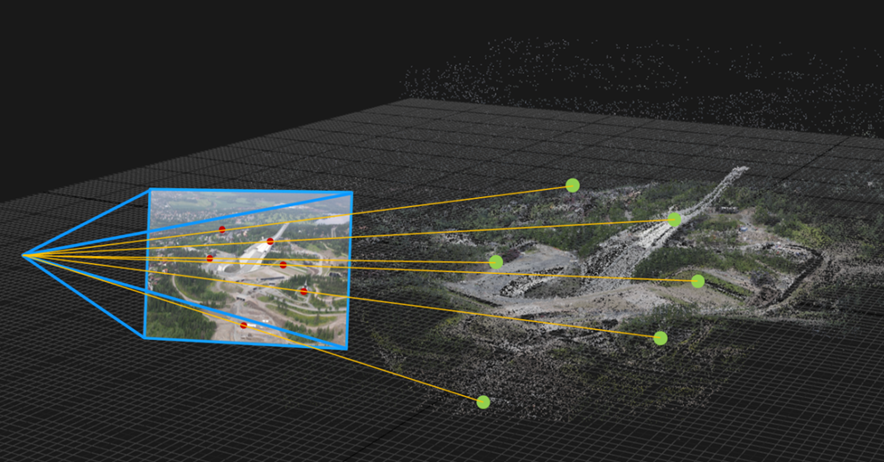
\includegraphics[width=\columnwidth]{figures/moba.png}
    \caption{An example of estimating pose from correspondences between pixel points and 3D points in a map.
    }
    \label{fig:moba}
\end{figure}

This chapter gives a brief introduction to how we can estimate pose and structure from images, based on the principles we have covered in the previous chapters.

Pose estimation using cameras is also sometimes called \emph{motion estimation} or \emph{localisation}, and is usually estimated relative to known structure, as illustrated in Figure~\ref{fig:moba}.
The \emph{structure} is here a representation of the 3D structure in the scene, which is also sometimes called a \emph{map}.
When we know the relative poses between two or more cameras, we can estimate the structure by triangulating correspondences between the cameras.

When neither pose nor structure is known a priori, we typically need to \emph{initialise} a map based on relative pose estimates between camera images.
We can then estimate new poses relative to this map, and continue extending the map while exploring the scene.
This procedure is often called \emph{simultaneous localisation and mapping (SLAM)}, and performing SLAM with images is often called \emph{Visual SLAM (VSLAM)}.

A major problem with monocular vision is that scale in the world cannot be observed without prior knowledge. 
Monocular VSLAM will therefore drift in scale over time, and this results in a major contribution to the overall error. 
But as pointed out in \cite{Engel2014LSD-SLAM:SLAM}, an interesting paradox is that its inherent scale-ambiguity is also a major benefit, since monocular vision can seamlessly operate in vastly differently scaled environments, such as switching from a small-scale door handle to the large-scale environment just outside.

Adding more sensors, such as another camera with known baseline, active range sensors or an inertial navigation system, can enable us to recover metric scale, as well as the horizontal plane, and even the geographical pose.

\section{Problem formulations}
It is common to formulate pose estimation problems as either \emph{direct} or \emph{indirect}, and structure estimation problems as either \emph{dense} or \emph{sparse} \cite{Engel2018}.

\emph{Indirect methods} first extract an intermediate geometrical representation of the scene, such as keypoint correspondences or optical flow vectors, and use these to optimise a \emph{geometric error}.
Because these methods are based on some kind of feature extraction step, they are also often called \emph{feature-based methods}.
Indirect methods provide robustness to photometric and geometric distortions, but come at the price of higher computational cost and are dependent on the feature extraction step to work.

\emph{Direct methods} skip the feature extraction step, and use the image intensity values directly to optimise a \emph{photometric error}.
Direct methods do not require that geometrical primitives are recognisable by themselves, but can sample across all parts of the image.
This makes direct methods more robust to effects such as motion blur and better suited in environments that are sparsely textured, but they are vulnerable to photometric and geometric distortions.

\emph{Sparse methods} reconstruct and use only a selected set of independent points in the scene, while \emph{dense methods} attempt to reconstruct and use a 3D map for all the pixels in the images.
An important difference between the sparse and dense methods is that, while the sparse methods map independent points with no notion of neighbourhoods, the dense methods typically add a geometric prior, assuming that the structure is locally smooth.
Because of the resulting correlated structure in the dense maps, it is difficult to optimise pose and dense structure jointly in real-time.

The most widely used formulation is the sparse indirect formulation, which is used in methods such as PTAM \cite{Klein2007ParallelWorkspaces} and ORB-SLAM \cite{Mur-Artal2015ORB-SLAM:System}.
The sparse direct formulation is used in DSO \cite{Engel2018}, while the dense direct formulation is used in DTAM \cite{Newcombe2011DTAM:Real-time} and LSD-SLAM \cite{Engel2014LSD-SLAM:SLAM}.
SVO \cite{Forster2014SVO:Odometry} uses a hybrid formulation, where the direct formulation is used for initial alignment and to obtain correspondences, while the indirect formulation is used for joint model optimisation.

We will in the following sections take a closer look at how we can express and solve some of these problems.


\section{Indirect methods}
We will here consider sparse, indirect methods based on point correspondence measurements between images.
Given correspondences $\vecu \leftrightarrow \vecx^w$ between pixels and points in the world frame (defined by the map), these methods minimise the \emph{geometric error}, which for each correspondence can be expressed as
\begin{equation}
  e_g(\matT_{wc}, \vecx^w) = \pi_p(\matT_{wc}^{-1} \cdot \vecx^w) - \vecu.
\end{equation}
Here, $\pi_p$ is the projection function for the perspective camera given in \eqref{eq:projection-function} and $\matT_{wc}$ is the pose of the camera in the world frame.
The geometric error measures the difference between the predicted pixel position, given the current hypotheses for the pose $\matT_{wc}$ and the point $\vecx^w$, and the measured pixel correspondence.
It is therefore also often called the \emph{reprojection error}.
Estimating poses and structure based on the geometric error is often called \emph{bundle adjustment} \cite{Triggs2000BundleSynthesis}.

The following sections will discuss how we can estimate pose, structure and both, based on minimising the geometric error.

\subsection{Estimating pose with known structure}
Assume that the world points $\vecx^w_j$ are known, and we are given the correspondences $\vecu_j \leftrightarrow \vecx^w_j$, with measurement noise $\matSigma_j$.

A suitable initial estimate for the pose $\matT_{wc}$ can be found by applying a fast \emph{perspective-n-point (PnP)} algorithm, such as P3P \cite{Kneip2011AOrientation}.
Estimating the camera pose from known 3D points by minimising the geometric error is sometimes called \emph{motion-only bundle adjustment}.
Assuming that the camera is calibrated, we can pre-calibrate the measurements to normalised image coordinates with \eqref{eq:normalised-from-pixel}.
This gives us the measurement prediction function
\begin{equation}
  h_j(\matT_{wc}) = \pi_n(\matT_{wc}^{-1} \cdot \vecx^w_j),
\end{equation}
where $\pi_n$ is the projection function to normalised image coordinates in \eqref{eq:normalised-projection-function}.
The measurement error function is the geometric error
\begin{equation}
  e_j(\matT_{wc}) = \pi_n(\matT_{wc}^{-1} \cdot \vecx^w_j) - \vecx_{n \; j}.
\end{equation}

The Jacobian of the measurement prediction function is given by (omitting the index $j$ for brevity)
\begin{subequations} \label{eq:ba-pose-jacobian}
\begin{align}
  \jac{h}{\matT_{wc}} &= \jac{\pi_n(\matT_{wc}^{-1} \cdot \vecx^w)}{\matT_{wc}^{-1} \cdot \vecx^w} \jac{\matT_{wc}^{-1} \cdot \vecx^w}{\matT_{wc}^{-1}} \jac{\matT_{wc}^{-1}}{\matT_{wc}}\\
  &= \jac{\pi_n(\vecx^c)}{\vecx^c} \jac{\matT_{wc}^{-1} \cdot \vecx^w}{\matT_{wc}^{-1}} \jac{\matT_{wc}^{-1}}{\matT_{wc}}\\
  &= \frac{1}{z^c}
  \begin{bmatrix}
  1 & 0 & -x^c/z^c\\
  0 & 1 & -y^c/z^c
  \end{bmatrix}
  \begin{bmatrix}
    \matR_{wc}\trans & -\matR_{wc}\trans \skewsymm{\vecx^w}
  \end{bmatrix}
  \cdot
  -\begin{bmatrix}
    \matR_{wc} & \skewsymm{\vect^w_{wc}} \matR_{wc}\\
    \matr{0} & \matR_{wc}
  \end{bmatrix}\\
  &= d
  \begin{bmatrix}
  1 & 0 & -x_n\\
  0 & 1 & -y_n
  \end{bmatrix}
  \begin{bmatrix}
  -\matI & \skewsymm{\vecx^c}
  \end{bmatrix}\\
  &=
  \begin{bmatrix}
    -d & 0 & dx_n & x_n y_n & -1-x^2_n & y_n\\
    0 & -d & dy_n & 1 + y^2_n & -x_n y_n & -x_n
  \end{bmatrix},
\end{align}
\end{subequations}
where $\vecx^c = \matT_{wc}^{-1} \cdot \vecx^w$ is the point in camera frame, and $d = 1/z^c$ is the inverse depth.

By propagating the noise to the normalised image plane, we get the linearised weighted least squares problem
\begin{align}
  \vecxi^\ast &= \argmin_{\vecxi} \sum^n_{j=1} \norm{ \matA_j \vecxi - \vecb_j}^2\\
  &= \argmin_{\vecxi} \norm{ \matA \vecxi - \vecb}^2,
\end{align}
where
\begin{align}
  \matA_j &= \matSigma^{-1/2}_{n \; j} \jac{h_j}{\matT_{wc}}\\
  \vecb_j &= \matSigma^{-1/2}_{n \; j} (\vecx_{n \; j} - h_j(\matT_{wc})),
\end{align}
and
\begin{equation}
  \matA =  
  \begin{bmatrix}
    \matA_1\\
    \vdots\\
    \matA_n
  \end{bmatrix}
  \qquad
  \vecb =  
  \begin{bmatrix}
    \vecb_1\\
    \vdots\\
    \vecb_n
  \end{bmatrix}.
\end{equation}

This lets us compute the MAP estimate $\hat{\matT}_{wc}$ with Gauss-Newton or Levenberg-Marquardt.

\subsection{Estimating structure with known poses}
Assume that we know the poses of the two or more cameras $\{ \matT_{wc_i}\}$, and we are given the correspondences $\vecu^i_j \leftrightarrow \vecx^w_j$, with measurement noise $\matSigma_{ij}$.

A suitable initial estimate for the structure $\{ \vecx^w_j \}$ can be found by for example triangulating the points linearly by minimising algebraic error \cite{Hartley2004MultipleVision}.
Estimating the structure from known camera poses by minimising the geometric error is sometimes called \emph{structure-only bundle adjustment}.
Assuming that the cameras are calibrated, we can pre-calibrate the measurements to normalised image coordinates with \eqref{eq:normalised-from-pixel}.
This gives us the measurement prediction function
\begin{equation}
  h_{ij}(\vecx^w_j) = \pi_n(\matT_{wc_i}^{-1} \cdot \vecx^w_j),
\end{equation}
where $\pi_n$ is the projection function to normalised image coordinates in \eqref{eq:normalised-projection-function}.
The measurement error function is the geometric error
\begin{equation}
  e_{ij}(\vecx^w_j) = \pi_n(\matT_{wc_i}^{-1} \cdot \vecx^w_j) - \vecx_{n \; j}^i.
\end{equation}

The Jacobian of the measurement prediction function is given by (omitting the indexes $i$ and $j$ for brevity)
\begin{subequations} \label{eq:ba-structure-jacobian}
\begin{align}
  \jac{h}{\vecx^w} &= \jac{\pi_n(\matT_{wc}^{-1} \cdot \vecx^w)}{\matT_{wc}^{-1} \cdot \vecx^w} \jac{\matT_{wc}^{-1} \cdot \vecx^w}{\vecx^w}\\
  &= \jac{\pi_n(\vecx^c)}{\vecx^c}  \jac{\matT_{wc}^{-1} \cdot \vecx^w}{\vecx^w}\\
  &= \frac{1}{z^c}
  \begin{bmatrix}
  1 & 0 & -x^c/z^c\\
  0 & 1 & -y^c/z^c
  \end{bmatrix}
  \matR_{wc}\trans\\
  &= d
  \begin{bmatrix}
  1 & 0 & -x_n\\
  0 & 1 & -y_n
  \end{bmatrix}
  \matR_{wc}\trans,
\end{align}
\end{subequations}
where $\vecx^c = \matT_{wc}^{-1} \cdot \vecx^w$ is the point in camera frame, and $d = 1/z^c$ is the inverse depth.

By propagating the noise to the normalised image plane, we get the linearised weighted least squares problem
\begin{align}
  \delta\vecx^\ast &= \argmin_{\delta\vecx} \sum^k_{i=1} \sum^n_{j=1} \norm{ \matA_{ij} \delta\vecx_j - \vecb_{ij}}^2\\
  &= \argmin_{\delta\vecx} \norm{ \matA \delta\vecx - \vecb}^2,
\end{align}
where
\begin{align}
  \matA_{ij} &= \matSigma^{-1/2}_{n \; {ij}} \jac{h_{ij}}{\vecx^w_j}\\
  \vecb_{ij} &= \matSigma^{-1/2}_{n \; {ij}} (\vecx_{n \; j}^i - h_{ij}(\vecx^w_j)),
\end{align}
and

\begin{equation}
  \matA =  
  \begin{bmatrix}
    \matA_{11} & & \\
    & \ddots & \\
    & & \matA_{1n}\\
    & \vdots &\\
    \matA_{k1} & & \\
    & \ddots & \\
    & & \matA_{kn}
  \end{bmatrix}
  \qquad  
  \delta\vecx =
  \begin{bmatrix}
    \delta\vecx_1\\
    \vdots\\
    \delta\vecx_n
  \end{bmatrix}
  \qquad
  \vecb =  
  \begin{bmatrix}
    \vecb_{11}\\
    \vdots\\
    \vecb_{1n}\\
    \vdots\\
    \vecb_{k1}\\
    \vdots\\
    \vecb_{kn}
  \end{bmatrix}.
\end{equation}

This lets us compute the MAP estimates $\{\hat{\vecx}^w_j\}$ with Gauss-Newton or Levenberg-Marquardt.


\subsection{Estimating pose and structure}
In this situation we do not know either the camera poses $\{ \matT_{wc_i}\}$ nor the world points $\{ \vecx^w_j \}$.
We are just given the correspondences $\vecu^i_j \leftrightarrow \vecx^w_j$, with measurement noise $\matSigma_{ij}$.

A suitable initial estimate can be found by first applying pairwise two-view relative pose estimation, based on estimating the essential matrix $\matE$ using the 5-point algorithm \cite{Nister2004AnProblem}, and decomposing it to obtain the relative pose \cite{Hartley2004MultipleVision}.
Estimating the both pose and structure by minimising the geometric error is sometimes called \emph{full bundle adjustment}.
Assuming that the cameras are calibrated, we can pre-calibrate the measurements to normalised image coordinates with \eqref{eq:normalised-from-pixel}.
This gives us the measurement prediction function
\begin{equation}
  h_{ij}(\matT_{wc_i}, \vecx^w_j) = \pi_n(\matT_{wc_i}^{-1} \cdot \vecx^w_j),
\end{equation}
where $\pi_n$ is the projection function to normalised image coordinates in \eqref{eq:normalised-projection-function}.
The measurement error function is the geometric error
\begin{equation}
  e_{ij}(\matT_{wc_i}, \vecx^w_j) = \pi_n(\matT_{wc_i}^{-1} \cdot \vecx^w_j) - \vecx_{n \; j}^i.
\end{equation}

Since the measurement function is a function of two variables, we linearise it at the current state estimates as
\begin{subequations}
\begin{align}
    h_{ij}(\matT_{wc_i}, \vecx^w_j) &= h_{ij}(\hat{\matT}_{wc_i} \oplus \vecxi_i, \hat{\vecx}^w_j + \delta\vecx_j) \\
    &\approx h_{ij}(\hat{\matT}_{wc_i}, \hat{\vecx}^w_j) + \jac{h_{ij}}{\hat{\matT}_{wc_i}}\vecxi_i + \jac{h_{ij}}{\hat{\vecx}^w_j}\delta\vecx_j,
\end{align}
\end{subequations}
The Jacobians are given in \eqref{eq:ba-pose-jacobian} and \eqref{eq:ba-structure-jacobian}.

By propagating the noise to the normalised image plane, we get the linearised weighted least squares problem
\begin{align}
  \ubar{\vectau}^\ast &= \argmin_{\ubar{\vectau}} \sum^k_{i=1} \sum^n_{j=1} \norm{ \matP_{ij} \vecxi_i + \matS_{ij} \delta\vecx_j - \vecb_{ij}}^2\\
  &= \argmin_{\ubar{\vectau}} \norm{ \matA \ubar{\vectau} - \vecb}^2,
\end{align}
where
\begin{align}
  \matP_{ij} &= \matSigma^{-1/2}_{n \; {ij}} \jac{h_{ij}}{\matT_{wc_i}}\\
  \matS_{ij} &= \matSigma^{-1/2}_{n \; {ij}} \jac{h_{ij}}{\vecx^w_j}\\
  \vecb_{ij} &= \matSigma^{-1/2}_{n \; {ij}} (\vecx_{n \; j}^i - h_{ij}(\matT_{wc_i}, \vecx^w_j)),
\end{align}
and
\begin{equation} \label{eq:ba-matrices}
  \matA =  
  \begin{bmatrix}
    \matP_{11} &  &  & \matS_{11} & & \\
    \vdots & & & & \ddots & \\
    \matP_{1n} & & & & &\matS_{1n}\\
    & \ddots &  & & \vdots &\\
    & & \matP_{k1} & \matS_{k1} & & \\
    & & \vdots & & \ddots & \\
    & & \matP_{kn}& & &\matS_{kn}
  \end{bmatrix}
  \qquad  
  \ubar{\vectau} =
  \begin{bmatrix}
    \vecxi_1\\
    \vdots\\
    \vecxi_k\\
    \delta\vecx_1\\
    \vdots\\
    \delta\vecx_n
  \end{bmatrix}
  \qquad
  \vecb =  
  \begin{bmatrix}
    \vecb_{11}\\
    \vdots\\
    \vecb_{1n}\\
    \vdots\\
    \vecb_{k1}\\
    \vdots\\
    \vecb_{kn}
  \end{bmatrix}.
\end{equation}

The linear least squares problem in \eqref{eq:ba-matrices} is not uniquely determined and has a singular approximation to the Hessian.
This is because the global frame and scale is not defined, so we can apply any similarity transform to the camera poses without affecting the objective function.
This is sometimes called \emph{gauge freedom}.
We fix this by adding priors on at least one pose, defining the global frame, and at least one point, defining the global scale.

This lets us compute the MAP estimates $\{\hat{\matT}_{wc_i}\}$ and $\{\hat{\vecx}^w_j\}$ with Gauss-Newton or Levenberg-Marquardt.


\section{Direct methods} \label{sec:direct-methods}
We will here consider direct methods that optimise structure separately from pose.

Consider two images $I_a(\vecu)$ and $I_b(\vecu)$.
Given the relative pose $\matT_{ab}$ between the two cameras $a$ and $b$, we can define the \emph{warp function} \cite{Baker2004Lucas-KanadeFramework}
\begin{equation}
  \vecu^a = w(\vecu^b, z^b, \matT_{ab}) = \pi_p(\matT_{ab} \cdot  \pi_p^{-1}(\vecu^b, z^b)),
\end{equation}
that maps a pixel $\vecu^b$ in image $I_b$ to a pixel $\vecu_a$ in image $I_a$.
This lets us define the \emph{photometric error} between these two images at a given pixel as
\begin{equation} \label{eq:photometric-error}
  e_p(\vecu^b, z^b, \matT_{ab}) = I_a(w(\vecu^b, z^b, \matT_{ab})) - I_b(\vecu^b).
\end{equation}

Direct methods typically represent structure as a sparse or dense depth map for pixels rather than 3D points.
The depth is typically represented as the \emph{inverse depth} $d = z^{-1}$, because the inverse depth parameterisation is better suited when we want to model the uncertainty in depth using a Gaussian noise model \cite{Civera2012InverseParametrization}.
Depth can be estimated by collecting small-baseline measurements over time, letting the uncertainty in depth fall below a threshold before using it for pose estimation \cite{Engel2013Semi-denseCamera, Engel2014LSD-SLAM:SLAM, Forster2014SVO:Odometry}.

If we know the pose $\matT_{ab}$ between the two images, we can exploit the epipolar geometry to search for good matches that minimises \eqref{eq:photometric-error} over a relevant interval of depths, guided by the current depth uncertainty (Section~\ref{sec:epipolar-geometry}).
Since
\begin{equation}
  z^a \matK^{-1}_a \breve{\vecu}^a = z^b \matR_{ab} \matK^{-1}_b \breve{\vecu}^b + \vect^a_{ab},
\end{equation}
we can compute both depths by solving the linear least squares problem
\begin{equation}
  \vecz^\ast = \argmin_\vecz \norm{\matA\vecz - \vecb}^2,
\end{equation}
where
\begin{equation}
  \matA = 
  \begin{bmatrix}
    \matK^{-1}_a \breve{\vecu}^a & -\matR_{ab} \matK^{-1}_b \breve{\vecu}^b
  \end{bmatrix}
  \qquad
  \vecz = 
  \begin{bmatrix}
    z^a\\
    z^b
  \end{bmatrix}
  \qquad
  \vecb = \vect^a_{ab}.
\end{equation}

When interested in $z^j$ only, the law of sines applied on the epipolar plane gives us
\begin{equation}
  z^b = \frac{\norm{\matK_a^{-1} \breve{\vecu}^a \times \vect^a_{ab}}} {\norm{\matK_a^{-1} \breve{\vecu}^a \times \matR_{ab} \matK^{-1}_b \breve{\vecu}^b}}.
\end{equation}
We can avoid the computations of the norms by
\begin{equation}
  z^b = \frac{\veca\trans (\matK_a^{-1} \breve{\vecu}^a \times \vect^a_{ab})} {\veca\trans (\matK_a^{-1} \breve{\vecu}^a \times \matR_{ab} \matK^{-1}_b \breve{\vecu}^b)},
\end{equation}
where $\veca \in \bbR^3$ is a suitable vector that is not perpendicular to the epipolar plane, or parallel to any of the vectors in the cross products.

Assuming that the cameras are calibrated, we can pre-calibrate the measurements to normalised image coordinates with \eqref{eq:normalised-from-pixel}.
This results in the warp function
\begin{equation}
  w_n(\vecx^b_n, z^b, \matT_{ab})) = \pi_n(\matT_{ab} \cdot \pi_n^{-1}(\vecx^b_n, z^b)).
\end{equation}
Given the depths $\{z^b_i\}$ for normalise image coordinates $\{\vecx^b_{n \; i}\}$ and the images $I_a$ and $I_b$, we can estimate the pose $\matT_{ab}$ by defining the measurement prediction function for the pixel intensity in image $I_b$ as
\begin{equation}
  h_i(\matT_{ab}) = I_a(w_n(\vecx^b_{n \; i}, z^b_i, \matT_{ab})),
\end{equation}
and the measurement error function as
\begin{equation}
 e_i(\matT_{ab}) = I_a(w_n(\vecx^b_{n \; i}, z^b_i, \matT_{ab})) - I_b(\vecx^b_{n \; i}).
\end{equation}

The Jacobian of the measurement prediction function is given by (omitting the indexes $i$ for brevity)
\begin{subequations} \label{eq:direct-pose-jacobian}
\begin{align}
  \jac{h}{\matT_{ab}} &= \jac{I_a}{w_n(\vecx^b_n, z^b, \matT_{ab})} \jac{w_n(\vecx^b_n, z^b, \matT_{ab})}{\matT_{ab}}\\
  &= \jac{I_a}{\pi_n(\vecx^a)} \jac{\pi_n(\matT_{ab} \cdot \vecx^b)}{\matT_{ab} \cdot \vecx^b} \jac{\matT_{ab} \cdot \vecx^b}{\matT_{ab}}\\
  &= \jac{I_a}{\vecx^a_n} \jac{\pi_n(\vecx^a)}{\vecx^a} \jac{\matT_{ab} \cdot \vecx^b}{\matT_{ab}}\\
  &= \nabla I_a(\vecx^a_n) \;
   d
  \begin{bmatrix}
  1 & 0 & -x^a_n\\
  0 & 1 & -y^a_n
  \end{bmatrix}
  \begin{bmatrix}
    \matR_{ab} & -\matR_{ab} \skewsymm{\vecx^b}
  \end{bmatrix},
\end{align}
\end{subequations}
where $\nabla I_a(\vecx^a_n)$ is the image gradient at $\breve{\vecu}^a = \matK_a \breve{\vecx}^a_n$.

This lets us compute the MAP estimate $\hat{\matT}_{ab}$ with Gauss-Newton or Levenberg-Marquardt.

% \section{Structure from Motion and Visual SLAM} \label{sec:sfm-and-vslam}
% \begin{figure}[htb]
%     \centering
%     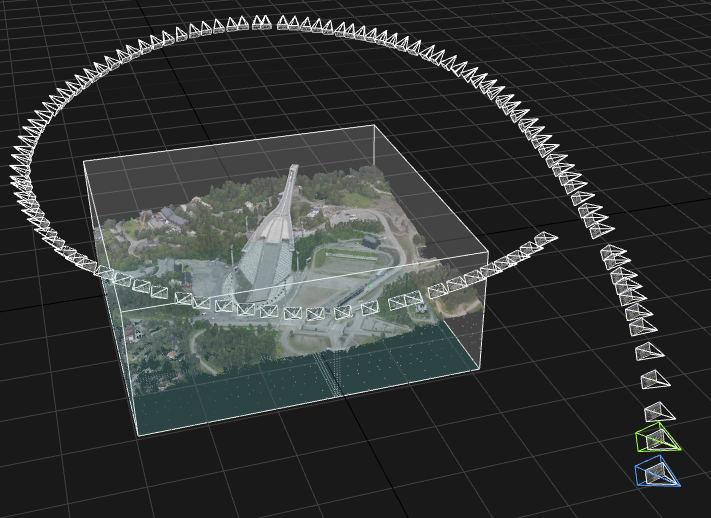
\includegraphics[width=0.75\columnwidth]{figures/holmenkollen-3d.png}
%     \caption{An example of structure from motion and 3D reconstruction based only on the images themselves.
%     }
%     \label{fig:sfm}
% \end{figure}
% Two different research fields in particular have been involved in studying methods for estimating motion and scene structure simultaneously using cameras, which is a difficult and highly nonlinear problem.

% The SLAM field within robotics have traditionally been using sequential filtering methods \cite{Thrun2002ProbabilisticRobotics} to estimate the real-time motion of robots and the position of landmarks, often in combination with other sensors.
% Traditional nonlinear filtering methods, such as the EKF\footnote{Extended Kalman Filter}, achieve fast estimation rates by updating just based on the current states, since previous states are marginalised out when new states are added.
% These methods also choose linearisation points for new states at the current time, and maintain these linearisations throughout the estimation.
% This will cause linearisation errors that accumulate over time, causing the solution to drift and the filter to become inconsistent.

% The structure from motion (SFM) field in computer vision has evolved from photogrammetry, and has traditionally focused their work on offline 3D reconstruction of the environment based on batch optimisation through \textit{bundle adjustment} \cite{Triggs2000BundleSynthesis}.
% Smoothing approaches such as this are generally more accurate than filtering, since they are able to relinearise past measurements.
% In addition, by keeping past states it is easy to add measurements with high latency and to perform loop closures when areas are revisited.
% The last 10 years or so has seen the bridging of the gap between these two fields, where the de-facto standard now is to formulate the mapping problem as a batch MAP estimation problem \cite{Strasdat2012VisualFilter, Cadena2016}, typically based on \emph{factor graphs}.

% \begin{figure}[htb]
%     \centering
%     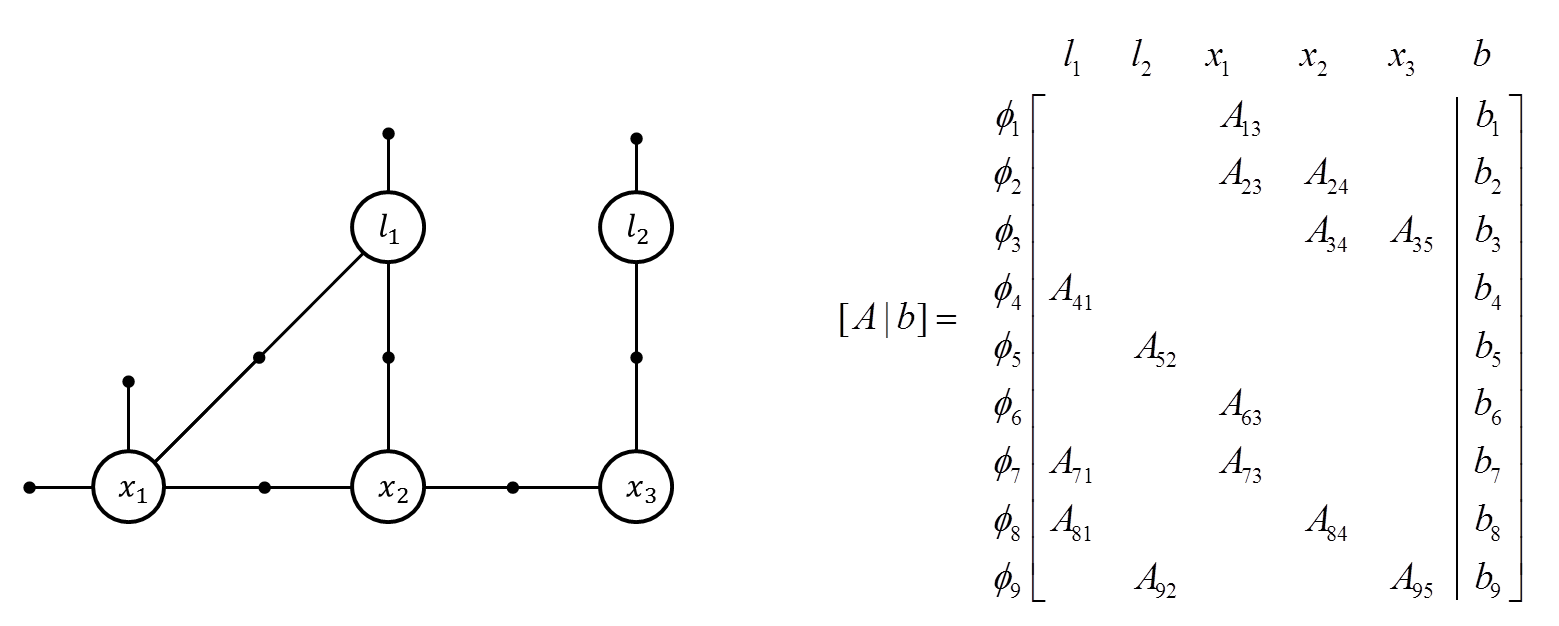
\includegraphics[width=\columnwidth]{figures/factor-graph-structure.png}
%     \caption{An example of a factor graph for a simple SLAM problem. 
%     On the left we see a visualisation of the factor graph.
%     Circles denote the state variable nodes for the poses $x_i$ and the landmark positions $l_j$. 
%     The black dots represent the factors corresponding to priors and measurements on the variables. 
%     The unary factors on $x_1$, $l_1$ and $l_2$ correspond to priors on these variables, while $x_1$ has an additional unary factor corresponding to a GPS measurement. 
%     The binary factors between poses represent odometry measurements, while the factors between poses and landmarks are bearing measurements.
%     The matrix to the right shows how the graph encodes the structure of the Jacobian $\matA$.
%     }
%     \label{fig:factor-graphs}
% \end{figure}
% A factor graph represents the estimation problem as a graphical model, and provides powerful tools for expressing and solving nonlinear estimation problems \cite{Dellaert2017}.
% It lets us specify constraints on state variables directly in a modular way, by specifying measurement prediction functions and Jacobians.
% The graph encodes dependencies directly, implicitly representing large sparse Jacobian matrices like \eqref{eq:ba-structure-jacobian}, by working only on the relevant blocks (Figure~\ref{fig:factor-graphs}).
% The estimation procedure is usually based on nonlinear least squares, as presented in Chapter~\ref{ch:nls}.

% It is customary to separate a SLAM system into two main components: the \emph{front end} and the \emph{back end} \cite{Cadena2016}.
% The front end extracts relevant data and data associations from raw sensor measurements, while the back end performs estimation and inference on data from the front end.
% Since the introduction of the ground breaking VSLAM system \emph{Parallel Tracking and Mapping} (PTAM) by Klein and Murray \cite{Klein2007ParallelWorkspaces}, VSLAM architectures are typically separated into a front end \emph{tracking} component, which estimates camera motion by tracking the scene structure using a map, and a back end \emph{mapping} component that builds the map based on observations.
% The key insight here was that these two components could be executed separately in different threads, allowing real-time pose estimation for each consecutive frame, while simultaneously updating and optimising the map at a lower rate on a selected set of spatially distributed \emph{keyframes}.

% In visual SLAM, the variables $X$ are often 3D camera poses and landmark positions.
% The factors between the pose variables and the landmark variables encode the errors in the predicted landmark projections for each camera using the current hypothesis $X^k$, compared to the actual measurements $Z$.
% The prior factors on camera poses and landmark positions encode the errors in the assumed state compared to the hypothesis.
% Given an appropriate motion model, for example, factors between camera poses can also be defined.
% In fact, by defining appropriate measurement prediction functions and Jacobians, any additional constraints between variables based on measurements from other sources, such as IMUs, GNSS, barometers and lidars \cite{Chiu2014}, can also be included in the optimisation as new factors.
% Additional variables such as calibration parameters can similarly be included by extending the measurement models.
% This is what makes the factor graph framework a powerful tool for VSLAM and data fusion in general.

% Factor graph implementations \cite{Kummerle2011G2o:Optimization, KuemmerleG2oSource, Dellaert2012FactorIntroduction, Dellaert2018GTSAMSource} provide \emph{full batch} solvers based on sparse linear algebra, that can be used in real time in the PTAM architecture.
% This can be combined with \emph{fixed-lag smoothers} \cite{Strasdat2011DoubleSLAM, Chiu2013}, that achieves constant estimation time by performing optimisation over a fixed window of states, while marginalising out the rest.
% There are also incremental solvers that efficiently update the solution given new data \cite{Kaess2012ISAM2:Tree}.
% Full (incremental) smoothing and (incremental) fixed-lag smoothing may also be combined in what is called \textit{concurrent smoothing and mapping} \cite{Kaess2012, Chiu2013}, and allows constant-time estimation with full batch optimisation over the same factor graph.
% Finally, there are also solvers that relax the assumption on Gaussian noise, and may perform full batch and incremental inference over non-parametric multimodal distributions \cite{Fourie2016, Fourie2017Multi-modalGraphs, incrementalinferencejl}. 
% This is especially interesting when data associations are uncertain, for example when you know you are close to a house, but not which of several possible houses in a given prior map.
% The multimodal factor graph framework makes it possible to perform inference over multiple hypotheses in this situation, enabling the back end to exploit more information than would otherwise be possible.


%\chapter{SfM and VSLAM}
Two different research fields in particular have been involved in studying methods for estimating motion and scene structure simultaneously using cameras, which is a difficult and highly nonlinear problem.

The SLAM field within robotics have traditionally been using sequential filtering methods \cite{Thrun2002ProbabilisticRobotics} to estimate the real-time motion of robots and the position of landmarks, often in combination with other sensors.
Traditional nonlinear filtering methods, such as the EKF\footnote{Extended Kalman Filter}, achieve fast estimation time by updating just based on the current states, since previous states are marginalised out when new states are added.
These methods also choose linearisation points for new states at the current time, and maintain these linearisations throughout the estimation.
This will cause linearisation errors that accumulate over time, causing the solution to drift and the filter to become inconsistent.

The structure from motion (SFM) field in computer vision has evolved from photogrammetry, and has traditionally focused their work on offline 3D reconstruction of the environment based on batch optimisation through \textit{bundle adjustment} \cite{Triggs2000BundleSynthesis}.
Smoothing approaches such as this are generally more accurate than filtering, since they are able to relinearise past measurements.
In addition, by keeping past states it is easy to add measurements with high latency and to perform loop closures when areas are revisited.
The last 10 years or so has seen the bridging of the gap between these two fields, where the de-facto standard now is to formulate the mapping problem as a batch MAP estimation problem\cite{Strasdat2012VisualFilter, Cadena2016}, typically based on \textit{factor graphs}.

A factor graph represents the estimation problem as a graphical model, and provides powerful tools for expressing and solving nonlinear estimation problems \cite{Dellaert2017}.
It is a bipartite graph $F = (\mathcal{U}, \mathcal{V}, \mathcal{E})$, with two node types: \textit{factors} $\phi_i \in \mathcal{U}$ and \textit{variables} $x_j \in \mathcal{V}$.
Edges $e_{ij} \in \mathcal{E}$ are always between factor nodes and variable nodes.
The set of nodes adjacent to a factor $\phi_i$ is written as $\mathcal{N}(\phi_i)$, and we write $X_i$ for an assignment to this set.
A factor graph $F$ then defines the factorisation of a function $\phi(X)$ as
\begin{equation}
    \phi(X) = \prod_i{\phi_i(X_i)}. \label{eqn:factor}
\end{equation}
Independence relationships are encoded by the edges $e_{ij}$ of the factor graph, with each factor $\phi_i$ a function of \textit{only} the variables $X_i$ in its adjacency set $\mathcal{N}(\phi_j)$.

We can represent the posterior in \eqref{eqn:MAP} with a factor graph by letting $\phi(X) \propto p(X|Z)$. 
Since
\begin{equation}
    p(X|Z) \propto l(X;Z)p(X) = \prod_i l(X_i;Z_i) \prod_j p(x_j),
\end{equation}
each factor $\phi_i$ will then correspond to either prior densities $p(x_j)$ or likelihood functions $l(X_i;Z_i)$ from the factored unnormalised posterior. MAP inference then simply comes down to maximising the product (\ref{eqn:factor}) of all factor graph potentials:
\begin{align}
    X^{MAP} &= \argmax_X \phi(X)\\
            &= \argmax_X \prod_i \phi_i(X_i). \label{eqn:MAP_factors}
\end{align}
The measurements and priors can be modelled with a generative probabilistic model
\begin{equation}
    \hat{z}_i = h_i(X_i) + \eta_i,
\end{equation}
where $h_i(X_i)$ is the \textit{measurement prediction function} and $\eta_i$ is additive measurement noise.
If we assume Gaussian priors and likelihood functions derived from measurements corrupted by zero-mean normally distributed noise, all factors in (\ref{eqn:MAP_factors}) are of the form
\begin{equation}
    \phi_i(X_i) \propto \exp \left \{ - \frac{1}{2} \norm{h_i(X_i) - z_i}_{\Sigma_i}^2 \right \},
\end{equation}
where
\begin{equation}
    \norm{e}_{\Sigma}^{2} \triangleq e^T \Sigma^{-1} e
\end{equation}
denotes the squared Mahalanobis distance over the \textit{residual errors}.

By taking the negative log of (\ref{eqn:MAP_factors}) and dropping the constant factor, we can instead minimise a sum of nonlinear least-squares:
\begin{equation}
    X^{MAP} = \argmin_x \sum_i \norm{h_i(X_i) - z_i}_{\Sigma_i}^2. \label{eqn:nonlinear_ls}
\end{equation}
MAP inference in this situation is therefore equivalent to solving a nonlinear least-squares problem,
and can be efficiently computed using iterative nonlinear optimisation methods such as Gauss-Newton or Levenberg-Marquardt, given a good initial estimate $X^0_i$ and the \textit{measurement Jacobian}
\begin{equation}
    H_i \triangleq \frac{\partial h_i(X_i)}{\partial X_i}.
\end{equation}

In visual SLAM, the variables $X$ are often 3D camera poses and landmark positions.
The factors between the pose variables and the landmark variables encode the errors in the predicted landmark projections for each camera using the current hypothesis $X^k$, compared to the actual measurements $Z$.
The prior factors on camera poses and landmark positions encode the errors in the assumed state compared to the hypothesis.
Given an appropriate motion model, for example, factors between camera poses can also be defined.
In fact, by defining appropriate measurement prediction functions and Jacobians, any additional constraints between variables based on measurements from other sources, such as IMUs, GNSS, barometers and lidars \cite{Chiu2014}, can also be included in the optimisation as new factors.
Additional variables such as calibration parameters can similarly be included by extending the measurement models.
This is what makes the factor graph framework a powerful tool for VSLAM and data fusion in general.

This project will use factor graphs as the primary framework for fusing sensor data, prior information and other possible data sources in the mapping back end. 
Implementations \cite{Kummerle2011G2o:Optimization, KuemmerleG2oSource, Dellaert2012FactorIntroduction, Dellaert2018GTSAMSource} provide \textit{full batch} solvers based on sparse linear algebra, that can be used in real time in the PTAM architecture.
This can be combined with \textit{fixed-lag smoothers} \cite{Strasdat2011DoubleSLAM, Chiu2013}, that achieves constant estimation time by performing optimisation over a fixed window of states, while marginalising out the rest.
There are also incremental solvers that efficiently update the solution given new data \cite{Kaess2012ISAM2:Tree}.
Full (incremental) smoothing and (incremental) fixed-lag smoothing may also be combined in what is called \textit{concurrent smoothing and mapping} \cite{Kaess2012, Chiu2013}, and allows constant-time estimation with full batch optimisation over the same factor graph.
Finally, there are also solvers that relax the assumption on Gaussian noise, and may perform full batch and incremental inference over non-parametric multimodal distributions \cite{Fourie2016, Fourie2017Multi-modalGraphs, incrementalinferencejl}. 
This is especially interesting when data associations are uncertain, for example when you know you are close to a house, but not which of several possible houses in a given prior map.
The multimodal factor graph framework makes it possible to perform inference over multiple hypotheses in this situation, enabling the back end to exploit more information than would otherwise be possible.

It is customary to separate a SLAM system into two main components: the \textit{front end} and the \textit{back end} \cite{Cadena2016}.
The front end extracts relevant data and data associations from raw sensor measurements, while the back end performs estimation and inference on data from the front end.
Since the introduction of the ground breaking VSLAM system \textit{Parallel Tracking and Mapping} (PTAM) by Klein and Murray \cite{Klein2007ParallelWorkspaces}, VSLAM architectures are typically separated into a front end \textit{tracking} component, which estimates camera motion by tracking the scene structure using a map, and a back end \textit{mapping} component that builds the map based on observations.
The key insight here was that these two components could be executed separately in different threads, allowing real-time pose estimation for each consecutive frame, while simultaneously updating and optimising the map at a lower rate on a selected set of spatially distributed \textit{keyframes}.
% \chapter{Visual SLAM front ends}

\section{Initialisation}
\begin{itemize}
    \item two-view, two-view planar, stereo, ...
    \item other sensors
\end{itemize}

\section{Short-term tracking}

\begin{itemize}
    \item indirect, direct, dense, sparse again? Probably not? Rather what is map, how to track?
    \item pros and cons
    \item Keyframes
    \item Windowed
\end{itemize}

\section{Visual place recognition}

% \chapter{Visual SLAM back ends}
Two different research fields in particular have been involved in studying methods for estimating motion and scene structure simultaneously using cameras, which is a difficult and highly nonlinear problem.
The SLAM field within robotics have traditionally been using sequential filtering methods \cite{Thrun2002ProbabilisticRobotics} to estimate the real-time motion of robots and the position of landmarks, often in combination with other sensors.
Traditional nonlinear filtering methods, such as the EKF\footnote{Extended Kalman Filter}, achieve fast estimation time by updating just based on the current states, since previous states are marginalised out when new states are added.
These methods also choose linearisation points for new states at the current time, and maintain these linearisations throughout the estimation.
This will cause linearisation errors that accumulate over time, causing the solution to drift and the filter to become inconsistent.

The structure from motion (SFM) field in computer vision has evolved from photogrammetry, and has traditionally focused their work on offline 3D reconstruction of the environment based on batch optimisation through \textit{bundle adjustment} \cite{Triggs2000BundleSynthesis}.
Smoothing approaches such as this are generally more accurate than filtering, since they are able to relinearise past measurements.
In addition, by keeping past states it is easy to add measurements with high latency and to perform loop closures when areas are revisited.
The last 10 years or so has seen the bridging of the gap between these two fields, where the de-facto standard now is to formulate the mapping problem as a batch MAP estimation problem\cite{Strasdat2012VisualFilter, Cadena2016}, typically based on \textit{factor graphs}.

A factor graph represents the estimation problem as a graphical model, and provides powerful tools for expressing and solving nonlinear estimation problems \cite{Dellaert2017}.
It is a bipartite graph $F = (\mathcal{U}, \mathcal{V}, \mathcal{E})$, with two node types: \textit{factors} $\phi_i \in \mathcal{U}$ and \textit{variables} $x_j \in \mathcal{V}$.
Edges $e_{ij} \in \mathcal{E}$ are always between factor nodes and variable nodes.
The set of nodes adjacent to a factor $\phi_i$ is written as $\mathcal{N}(\phi_i)$, and we write $X_i$ for an assignment to this set.
A factor graph $F$ then defines the factorisation of a function $\phi(X)$ as
\begin{equation}
    \phi(X) = \prod_i{\phi_i(X_i)}. \label{eqn:factor}
\end{equation}
Independence relationships are encoded by the edges $e_{ij}$ of the factor graph, with each factor $\phi_i$ a function of \textit{only} the variables $X_i$ in its adjacency set $\mathcal{N}(\phi_j)$.

We can represent the posterior in \eqref{eqn:MAP} with a factor graph by letting $\phi(X) \propto p(X|Z)$. 
Since
\begin{equation}
    p(X|Z) \propto l(X;Z)p(X) = \prod_i l(X_i;Z_i) \prod_j p(x_j),
\end{equation}
each factor $\phi_i$ will then correspond to either prior densities $p(x_j)$ or likelihood functions $l(X_i;Z_i)$ from the factored unnormalised posterior. MAP inference then simply comes down to maximising the product (\ref{eqn:factor}) of all factor graph potentials:
\begin{align}
    X^{MAP} &= \argmax_X \phi(X)\\
            &= \argmax_X \prod_i \phi_i(X_i). \label{eqn:MAP_factors}
\end{align}
The measurements and priors can be modelled with a generative probabilistic model
\begin{equation}
    \hat{z}_i = h_i(X_i) + \eta_i,
\end{equation}
where $h_i(X_i)$ is the \textit{measurement prediction function} and $\eta_i$ is additive measurement noise.
If we assume Gaussian priors and likelihood functions derived from measurements corrupted by zero-mean normally distributed noise, all factors in (\ref{eqn:MAP_factors}) are of the form
\begin{equation}
    \phi_i(X_i) \propto \exp \left \{ - \frac{1}{2} \norm{h_i(X_i) - z_i}_{\Sigma_i}^2 \right \},
\end{equation}
where
\begin{equation}
    \norm{e}_{\Sigma}^{2} \triangleq e^T \Sigma^{-1} e
\end{equation}
denotes the squared Mahalanobis distance over the \textit{residual errors}.

By taking the negative log of (\ref{eqn:MAP_factors}) and dropping the constant factor, we can instead minimise a sum of nonlinear least-squares:
\begin{equation}
    X^{MAP} = \argmin_x \sum_i \norm{h_i(X_i) - z_i}_{\Sigma_i}^2. \label{eqn:nonlinear_ls}
\end{equation}
MAP inference in this situation is therefore equivalent to solving a nonlinear least-squares problem,
and can be efficiently computed using iterative nonlinear optimisation methods such as Gauss-Newton or Levenberg-Marquardt, given a good initial estimate $X^0_i$ and the \textit{measurement Jacobian}
\begin{equation}
    H_i \triangleq \frac{\partial h_i(X_i)}{\partial X_i}.
\end{equation}

In visual SLAM, the variables $X$ are often 3D camera poses and landmark positions.
The factors between the pose variables and the landmark variables encode the errors in the predicted landmark projections for each camera using the current hypothesis $X^k$, compared to the actual measurements $Z$.
The prior factors on camera poses and landmark positions encode the errors in the assumed state compared to the hypothesis.
Given an appropriate motion model, for example, factors between camera poses can also be defined.
In fact, by defining appropriate measurement prediction functions and Jacobians, any additional constraints between variables based on measurements from other sources, such as IMUs, GNSS, barometers and lidars \cite{Chiu2014}, can also be included in the optimisation as new factors.
Additional variables such as calibration parameters can similarly be included by extending the measurement models.
This is what makes the factor graph framework a powerful tool for VSLAM and data fusion in general.

This project will use factor graphs as the primary framework for fusing sensor data, prior information and other possible data sources in the mapping back end. 
Implementations \cite{Kummerle2011G2o:Optimization, KuemmerleG2oSource, Dellaert2012FactorIntroduction, Dellaert2018GTSAMSource} provide \textit{full batch} solvers based on sparse linear algebra, that can be used in real time in the PTAM architecture.
This can be combined with \textit{fixed-lag smoothers} \cite{Strasdat2011DoubleSLAM, Chiu2013}, that achieves constant estimation time by performing optimisation over a fixed window of states, while marginalising out the rest.
There are also incremental solvers that efficiently update the solution given new data \cite{Kaess2012ISAM2:Tree}.
Full (incremental) smoothing and (incremental) fixed-lag smoothing may also be combined in what is called \textit{concurrent smoothing and mapping} \cite{Kaess2012, Chiu2013}, and allows constant-time estimation with full batch optimisation over the same factor graph.
Finally, there are also solvers that relax the assumption on Gaussian noise, and may perform full batch and incremental inference over non-parametric multimodal distributions \cite{Fourie2016, Fourie2017Multi-modalGraphs, incrementalinferencejl}. 
This is especially interesting when data associations are uncertain, for example when you know you are close to a house, but not which of several possible houses in a given prior map.
The multimodal factor graph framework makes it possible to perform inference over multiple hypotheses in this situation, enabling the back end to exploit more information than would otherwise be possible.


% \section{Mapping with factor graphs}
% \begin{itemize}
%     \item State estimation
%     \item Intro to factor graphs
%     \item GTSAM
% \end{itemize}


% \section{Batch VSLAM strategies}

% \section{Visual Odometry}


% \section{Incremental SLAM with factor graphs}


% \section{VSLAM and data fusion with other sensors}




% Appendices
\appendix
\chapter{Useful Lie groups} \label{ch:useful-lie-groups}
This appendix contains summaries of some of the most used Lie groups, and is heavily based on the appendix in \cite{SolaARobotics}.

\section{The 2D rotation group \SO(2)} \label{sec:SO2_group}
The \emph{special orthogonal group} in 2D is the set of valid $2 \times 2$ rotation matrices
\begin{equation}
  \SO(2) = \left \{ \matR \in \bbR^{2 \times 2} \;\middle|\; \matR\matR\trans = \matI, \det \matR = 1 \right \},
\end{equation}
where $\matR$ is on the form
\begin{equation}
  \matR = 
  \begin{bmatrix}
    \cos \theta & -\sin \theta \\
    \sin \theta & \cos \theta
  \end{bmatrix}.
\end{equation}
The group is closed under matrix multiplication with identity $\matI$.
Inversion is achieved with transposition
\begin{equation}
  \matR^{-1} = \matR\trans,
\end{equation}
and composition with the product
\begin{equation}
  \matR_a \circ \matR_b = \matR_a \matR_b.
\end{equation}
The group action on vectors $\vecx \in \bbR^2$ is given by the product
\begin{equation} \label{eq:SO2-group-action}
  \matR \cdot \vecx = \matR \vecx.
\end{equation}

\subsection{Lie algebra}
The Lie algebra of $\SO(2)$ is given by
\begin{equation}
  \so(2) = \left \{ \theta^\wedge = [\theta]_\times \in \bbR^{2 \times 2} \;\middle|\; \theta \in \bbR \right \},
\end{equation}
where
\begin{equation}
  [\theta]_\times \triangleq
  \begin{bmatrix}
    0 & -\theta \\
    \theta & 0
  \end{bmatrix}.
\end{equation}
The tangent space vector $\theta$ corresponds to the rotation angle, and since $\theta \in \bbR$, the dimension of \SO(2) is $m = 1$.

\subsection{Exp and Log maps} \label{sec:Exp-Log-SO2}
The $\Exp$ and $\Log$ maps for $\SO(2)$ is given by
\begin{align}
  \matR &= \Exp(\theta) = 
  \begin{bmatrix}
    \cos \theta & -\sin \theta \\
    \sin \theta & \cos \theta
  \end{bmatrix}\\
  \theta &= \Log(\matR) = \arctan(r_{21}, r_{11}).
\end{align}
Since
\begin{align}
  \matR(\theta)^{-1} &= \matR(-\theta)\\
  \matR_a \circ \matR_b &= \matR_b \circ \matR_a,
\end{align}
planar rotations are commutative.
It follows that
\begin{align}
  \Exp(\theta_a + \theta_b) &= \Exp(\theta_a) \circ \Exp(\theta_b)\\
  \Log(\matR_a \circ \matR_b) &= \Log(\matR_a) + \Log(\matR_b)\\
  \matR_b \ominus \matR_a &= \theta_b - \theta_a.
\end{align}
When $\theta$ is small, the following approximation holds:
\begin{equation} \label{eq:SO2-Exp-approx}
  \matR = \Exp(\theta) \approx \matI + \theta^\wedge.
\end{equation}

\subsection{The adjoint}
The adjoint matrix for $\SO(2)$ at $\matR$ is given by
\begin{equation}
  \mAd_\matR = 1 \in \bbR.
\end{equation}

\subsection{Jacobian blocks} \label{sec:Jacobians-SO2}
Most Jacobian blocks are scalar and trivial for $\SO(2)$.

\subsubsection*{Left and right Jacobians}
\begin{align}
\jac{}{r}(\theta) &= \jac{}{l}(\theta) = 1\\
\jac{}{r}^{-1}(\theta) &= \jac{}{l}^{-1}(\theta) = 1.
\end{align}

\subsubsection*{Jacobian of the inverse operation}
\begin{equation}
  \jac{\matR^{-1}}{\matR} = -1.
\end{equation}

\subsubsection*{Jacobians of the composition operation}
\begin{equation}
  \jac{\matR_a \matR_b}{\matR_a} = \jac{\matR_a \matR_b}{\matR_b} = 1.
\end{equation}

\subsubsection*{Jacobians of the plus and minus operators}
\begin{equation}
  \jac{\matR \oplus \theta}{\matR} = \jac{\matR \oplus \theta}{\theta} = 1.
\end{equation}
\begin{align}
  \jac{\matR_b \ominus \matR_a}{\matR_a} &= -1\\
  \jac{\matR_b \ominus \matR_a}{\matR_b} &= 1.
\end{align}

\subsubsection*{Jacobians of the group action}
\begin{align}
  \jac{\matR \cdot \vecx}{\matR} &= \matR [1]_\times \vecx\\
  \jac{\matR \cdot \vecx}{\vecx} &= \matR.
\end{align}

\section{The 3D rotation group \SO(3)} \label{sec:SO3_group}
The \emph{special orthogonal group} in 3D is the set of valid $3 \times 3$ rotation matrices
\begin{equation}
  \SO(3) = \left \{ \matR \in \bbR^{3 \times 3} \;\middle|\; \matR\matR\trans = \matI, \det \matR = 1 \right \},
\end{equation}
and is closed under matrix multiplication with identity $\matI$.
Inversion is achieved with transposition
\begin{equation}
  \matR^{-1} = \matR\trans,
\end{equation}
and composition with the product
\begin{equation}
  \matR_a \circ \matR_b = \matR_a \matR_b.
\end{equation}
The group action on vectors $\vecx \in \bbR^3$ is given by the product
\begin{equation} \label{eq:SO3-group-action}
  \matR \cdot \vecx = \matR \vecx.
\end{equation}

\subsection{Lie algebra}
The Lie algebra of $\SO(3)$ is given by
\begin{equation}
  \so(3) = \left \{ \vectheta^\wedge = [\vectheta]_\times \in \bbR^{3 \times 3} \;\middle|\; \vectheta \in \bbR^3 \right \},
\end{equation}
where the tangent space vector $\vectheta \triangleq \theta \vecu$ corresponds to the rotation on angle-axis form, with angle $\theta$ and unit rotation axis $\vecu$ (see Section~\ref{sec:orientation}).
Since $\vectheta \in \bbR^3$, the dimension of $\SO(3)$ is $m = 3$.

The Lie algebra is a vector space that can be decomposed into
\begin{equation}
  \vectheta^\wedge = [\vectheta]_\times = \theta_1 \matE_1 + \theta_2 \matE_2 + \theta_3 \matE_3,
\end{equation}
where
\begin{equation}
  \matE_1 =
  \begin{bsmallmatrix}
    0 & 0 & 0\\
    0 & 0 & -1\\
    0 & 1 & 0
  \end{bsmallmatrix}, \;
  \matE_2 =
  \begin{bsmallmatrix}
    0 & 0 & 1\\
    0 & 0 & 0\\
    -1 & 0 & 0
  \end{bsmallmatrix}, \;
  \matE_3 =
  \begin{bsmallmatrix}
    0 & -1 & 0\\
    1 & 0 & 0\\
    0 & 0 & 0
  \end{bsmallmatrix},
\end{equation}
are the generators of $\so(3)$. The hat and vee operators are given by
\begin{align}
\begin{alignedat}{2}
  \text{Hat} \; &: \quad \vectheta^\wedge &&= [\vectheta]_\times\\
  \text{Vee} \; &: \quad \vectheta &&= [\vectheta]^\vee_\times.
\end{alignedat}
\end{align}

\subsection{Exp and Log maps} \label{sec:Exp-Log-SO3}
Since the tangent space vector $\vectheta = \theta \vecu$ corresponds to the axis-angle representation, the $\Exp$ map is simply the Rodrigues' rotation formula
\begin{equation} \label{eq:Exp-SO3}
  \matR = \Exp(\vectheta) \triangleq \matI + \sin \theta [\vecu]_\times + (1 - \cos \theta) [\vecu]^2_\times.
\end{equation}

The $\Log$ map is given by
\begin{equation} \label{eq:Log-SO3}
  \vectheta = \Log(\matR) \triangleq \frac{\theta}{2 \sin \theta} (\matR - \matR\trans)^\vee,
\end{equation}
where
\begin{equation}
  \theta = \arccos \left( \frac{\tr(\matR) - 1}{2} \right).
\end{equation}

Special care must be taken when $\theta$ is small.
Practical implementations can in these cases use a Taylor expansion of the coefficient $\theta / (2 \sin \theta)$ \cite{Eade2013LieTransformations}.
Also, when $\theta$ is small, the following approximation holds (see \eqref{eq:infinitesimal-rotaton}):
\begin{equation} \label{eq:SO3-Exp-approx}
  \matR = \Exp(\vectheta) \approx \matI + \vectheta^\wedge.
\end{equation}

\subsection{The adjoint}
The adjoint matrix for $\SO(3)$ at $\matR$ is given by
\begin{equation}
  \mAd_\matR = \matR  \in \bbR^{3 \times 3}.
\end{equation}

\subsection{Jacobian blocks} \label{sec:Jacobians-SO3}
The right and left Jacobians, and their inverses, have the following closed form expressions: 
\begin{align}
\jac{}{r}(\vectheta) &= \matI - \frac{1-\cos\theta}{\theta^2}\skewsymm{\vectheta} + \frac{\theta-\sin\theta}{\theta^3}\skewsymm{\vectheta}^2\\
\jac{}{r}^{-1}(\vectheta) &= \matI + \frac{1}{2}\skewsymm{\vectheta} + \left(\frac{1}{\theta^2} - \frac{1+\cos\theta}{2\theta\sin\theta}\right)\skewsymm{\vectheta}^2 \\
\jac{}{l}(\vectheta) &= \matI + \frac{1-\cos\theta}{\theta^2}\skewsymm{\vectheta} + \frac{\theta-\sin\theta}{\theta^3}\skewsymm{\vectheta}^2 \label{eq:SO3-left-jac}\\
\jac{}{l}^{-1}(\vectheta) &= \matI - \frac{1}{2}\skewsymm{\vectheta} + \left(\frac{1}{\theta^2} - \frac{1+\cos\theta}{2\theta\sin\theta}\right)\skewsymm{\vectheta}^2.
\end{align}
Notice that
\begin{equation}
  \jac{}{l}(\vectheta) = \jac{}{r}(\vectheta)\trans, \quad\quad \jac{}{l}(\vectheta)^{-1} = \jac{}{r}(\vectheta)\invtrans.
\end{equation}

In the remainder of this section, we list the Jacobian blocks in Section~\ref{sec:elem-lie-blocks} developed for $\SO(3)$.

\subsubsection*{Jacobian of the inverse operation}
\begin{equation}
  \jac{\matR^{-1}}{\matR} = -\mAd_\matR = -\matR.
\end{equation}

\subsubsection*{Jacobians of the composition operation}
\begin{align}
  \jac{\matR_a \matR_b}{\matR_a} &= {\mAd_{\matR_b}}^{-1} = \matR_b\trans\\
  \jac{\matR_a \matR_b}{\matR_b} &= \matI.
\end{align}

\subsubsection*{Jacobians of the plus and minus operators}
\begin{align}
  \jac{\matR \oplus \vectheta}{\matR} &= {\mAd_{\Exp(\vectheta)}}^{-1} = \matR(\vectheta)\trans\\
  \jac{\matR \oplus \vectheta}{\vectheta} &= \jac{}{r}(\vectheta).
\end{align}
For $\vectheta = \matR_b \ominus \matR_a$, we have
\begin{align}
  \jac{\matR_b \ominus \matR_a}{\matR_a} &= -\jac{}{l}^{-1}(\vectheta)\\
  \jac{\matR_b \ominus \matR_a}{\matR_b} &= \jac{}{r}^{-1}(\vectheta).
\end{align}

\subsubsection*{Jacobians of the group action}
From Example~\ref{ex:lie-group-action-jac-SO3-example} we have
\begin{align}
  \jac{\matR \cdot \vecx}{\matR} &= -\matR [\vecx]_\times\\
  \jac{\matR \cdot \vecx}{\vecx} &= \matR.
\end{align}

\section{The 2D rigid motion group \SE(2)} \label{sec:SE2_group}
Coming, see \cite{SolaARobotics}.

\section{The 3D rigid motion group \SE(3)} \label{sec:SE3_group}
The \emph{special Euclidean group} in 3D is the set of valid Euclidean transformation matrices
\begin{equation}
  \SE(3) = \left \{ \matT =
  \begin{bmatrix}
    \matR & \vect\\
    \matr{0}\trans & 1
  \end{bmatrix}
  \in \bbR^{4 \times 4} \;\middle|\; \matR \in \SO(3), \vect \in \bbR^3 \right \},
\end{equation}
and is closed under matrix multiplication with identity $\matI$.
Inversion is given by
\begin{equation}
  \matT^{-1} = 
  \begin{bmatrix}
    \matR\trans & -\matR\trans \vect\\
    \matr{0}\trans & 1
  \end{bmatrix},
\end{equation}
and composition with the product
\begin{equation}
  \matT_a \circ \matT_b = \matT_a \matT_b = 
  \begin{bmatrix}
    \matR_a \matR_b & \matR_a \vect_b + \vect_a\\
    \matr{0}\trans & 1
  \end{bmatrix}.
\end{equation}
The group action on vectors $\vecx \in \bbR^3$ is given by
\begin{equation} \label{eq:SE3-group-action}
  \matT \cdot \vecx = \matT \tilde{\vecx} = \matR \vecx + \vect.
\end{equation}


\subsection{Lie algebra}
The Lie algebra of $\SE(3)$ is given by
\begin{equation}
  \se(3) = \left \{ \vecxi^\wedge = 
  \begin{bmatrix}
    [\vectheta]_\times & \vecrho\\
    \matr{0}\trans & 0
  \end{bmatrix}
  \in \bbR^{4 \times 4} \;\middle|\; \vecxi =
  \begin{bmatrix}
    \vecrho\\
    \vectheta
  \end{bmatrix}  
  \in \bbR^6 \right \},
\end{equation}
Since $\vecxi \in \bbR^6$, the dimension of $\SE(3)$ is $m = 6$.
The vectors $\vecrho, \vectheta \in \bbR^3$ correspond the translational and rotational parts, respectively.

The Lie algebra is a vector space that can be decomposed into
\begin{equation}
  \vecxi^\wedge = \xi_1 \matE_1 + \xi_2 \matE_2 + \xi_3 \matE_3 + \xi_4 \matE_4 + \xi_5 \matE_5 + \xi_6 \matE_6,
\end{equation}
where
\begin{equation}
\begin{alignedat}{3}
  &\matE_1 =
  \begin{bsmallmatrix}
    0 & 0 & 0 & 1\\
    0 & 0 & 0 & 0\\
    0 & 0 & 0 & 0\\
    0 & 0 & 0 & 0
  \end{bsmallmatrix}, \;
  &&\matE_2 =
  \begin{bsmallmatrix}
    0 & 0 & 0 & 0\\
    0 & 0 & 0 & 1\\
    0 & 0 & 0 & 0\\
    0 & 0 & 0 & 0
  \end{bsmallmatrix}, \;
  &&\matE_3 =
  \begin{bsmallmatrix}
    0 & 0 & 0 & 0\\
    0 & 0 & 0 & 0\\
    0 & 0 & 0 & 1\\
    0 & 0 & 0 & 0
  \end{bsmallmatrix},\\
  &\matE_4 =
  \begin{bsmallmatrix}
    0 & 0 & 0 & 0\\
    0 & 0 & -1 & 0\\
    0 & 1 & 0 & 0\\
    0 & 0 & 0 & 0
  \end{bsmallmatrix}, \;
  &&\matE_5 =
  \begin{bsmallmatrix}
    0 & 0 & 1 & 0\\
    0 & 0 & 0 & 0\\
    -1 & 0 & 0 & 0\\
    0 & 0 & 0 & 0
  \end{bsmallmatrix}, \;
  &&\matE_6 =
  \begin{bsmallmatrix}
    0 & -1 & 0 & 0\\
    1 & 0 & 0 & 0\\
    0 & 0 & 0 & 0\\
    0 & 0 & 0 & 0
  \end{bsmallmatrix},
\end{alignedat}
\end{equation}
are the generators of $\se(3)$. The hat and vee operators are given by
\begin{align}
\begin{alignedat}{2}
  \text{Hat} \; &: \quad \vecxi^\wedge &&= 
    \begin{bmatrix}
    [\vectheta]_\times & \vecrho\\
    \matr{0}\trans & 0
  \end{bmatrix}\\
  \text{Vee} \; &: \quad \vecxi &&=
    \begin{bmatrix}
    [\vectheta]_\times & \vecrho\\
    \matr{0}\trans & 0
  \end{bmatrix}^\vee.
\end{alignedat}
\end{align}

\subsection{Exp and Log maps}
The $\Exp$ map for $\SE(3)$ is given by
\begin{equation} \label{eq:SE3-exp}
  \matT = \Exp(\vecxi) \triangleq 
  \begin{bmatrix}
    \Exp(\vectheta) & \matV(\vectheta) \vecrho\\
    \matr{0}\trans & 1
  \end{bmatrix},  
\end{equation}
where $\Exp(\vectheta)$ is given by \eqref{eq:Exp-SO3} and 
\begin{equation}
  \matV(\vectheta) = \matI + \frac{1 - \cos \theta}{\theta}[\vecu]_\times + \frac{\theta - \sin \theta}{\theta} [\vecu]^2_\times.
\end{equation}

The $\Log$ map is given by
\begin{equation}
  \vecxi = \Log(\matT) \triangleq 
  \begin{bmatrix}
    \matV^{-1}(\vectheta) \vect\\
    \vectheta
  \end{bmatrix},
\end{equation}
where $\vectheta = \Log(\matR)$ from \eqref{eq:Log-SO3} and
\begin{equation}
  \matV^{-1}(\vectheta) = \matI - \frac{\theta}{2}[\vecu]_\times + \left(1 - \frac{\theta \sin \theta}{2(1 - \cos \theta)} \right)[\vecu]^2_\times.
\end{equation}

As for $\SO(3)$ in Section~\ref{sec:Exp-Log-SO3}, special care must be taken when $\theta$ is small \cite{Eade2013LieTransformations}.
Also, when $\theta$ is small, the following approximation holds:
\begin{equation} \label{eq:SE3-Exp-approx}
  \matT = \Exp(\vecxi) \approx \matI + \vecxi^\wedge.
\end{equation}

\subsection{The adjoint}
The adjoint matrix for $\SE(3)$ at $\matT$ is given by
\begin{equation}
  \mAd_\matT = 
  \begin{bmatrix}
    \matR & [\vect]_\times \matR\\
    \matr{0} & \matR
  \end{bmatrix} \in \bbR^{6 \times 6}.
\end{equation}

\subsection{Hybrid representation} \label{sec:hybrid-representation}
An alternative to representing poses on the $\SE(3)$ manifold, is to represent the orientation $\matR \in \SO(3)$ and position $\vect \in \bbR^3$ as two separate states without interaction.
Since $\vect$ is a vector, we will in this case only need to compute the $\Exp$ and $\Log$ maps for the orientation on the $\SO(3)$ manifold.

We can define maps the corresponding to $\Exp$ and $\Log$ for the hybrid representation as the pseudo-Exp and pseudo-Log maps \cite{BlancoAOptimization}:
\begin{align}
    \matT &= \text{pseudo-Exp}(\vecxi) \triangleq 
    \begin{bmatrix}
      \Exp(\vectheta) & \vecrho\\
      \matr{0}\trans & 1
  \end{bmatrix} \label{eq:SE3-pseudo-exp}\\ 
  \vecxi &= \text{pseudo-Log}(\matT) \triangleq 
  \begin{bmatrix}
    \vect\\
    \Log(\matR)
  \end{bmatrix}.
\end{align}

A \emph{retraction} is a more general way to define a mapping between the tangent space $\cT\cM$ and the manifold $\cM$ \cite{Forster2017, Dellaert2017, Absil2008OptimizationManifolds}.
For $\SE(3)$, the exponential map \eqref{eq:SE3-exp} is one example of retraction, while the pseudo-Exp \eqref{eq:SE3-pseudo-exp} is another, and sometimes more attractive choice.
This is because the pseudo-versions saves computations both for the $\Exp$ and $\Log$ maps, as well for the Jacobians.

\subsection{Jacobian blocks} \label{sec:Jacobians-SE3}
The left Jacobian and its inverse have the following closed form expressions: 
\begin{align}
\jac{}{l}(\vecxi) &= 
\begin{bmatrix}
  \jac{}{l}(\vectheta) & \matQ(\vecxi) \\
  \matr{0} & \jac{}{l}(\vectheta)
\end{bmatrix}\\
\jac{}{l}^{-1}(\vecxi) &= 
\begin{bmatrix}
  \jac{}{l}^{-1}(\vectheta) & -\jac{}{l}^{-1}(\vectheta) \matQ(\vecxi) \jac{}{l}^{-1}(\vectheta) \\
  \matr{0} & \jac{}{l}^{-1}(\vectheta)
\end{bmatrix}.  \label{eq:jacobian-left-inverse-SE3}
\end{align}
Here $\jac{}{l}(\vectheta)$ is the left Jacobian of $\SO(3)$ in \eqref{eq:SO3-left-jac} and $\matQ(\vecxi)$ is given by
%
\newcommand{\rhox}{\skewsymm{\vecrho}}
\newcommand{\thetax}{\skewsymm{\vectheta}}
%
\begin{equation}
\begin{split}
\matQ(\vecxi) =& 
  \frac{1}{2}\rhox 
  + \frac{\theta - \sin\theta}{\theta^3}(\thetax\rhox+\rhox\thetax+\thetax\rhox\thetax)\\
  &- \frac{1 - \frac{\theta^2}{2} - \cos\theta}{\theta^4}(\thetax^2\rhox+\rhox\thetax^2-3\thetax\rhox\thetax)\\
  &-\frac{1}{2}\left(\frac{1 -  \frac{\theta^2}{2} - \cos\theta}{\theta^4} 
                  - 3\frac{\theta-\sin\theta-\frac{\theta^3}{6}}{\theta^5}\right)
                  (\thetax\rhox\thetax^2 + \thetax^2\rhox\thetax).
\end{split}
\end{equation}
%
The right Jacobian and its inverse can be obtained using \eqref{eq:lie-right-jac-from-left}.

In the remainder of this section, we list the Jacobian blocks in Section~\ref{sec:elem-lie-blocks} developed for $\SE(3)$.

\subsubsection*{Jacobian of the inverse operation}
\begin{equation}
  \jac{\matT^{-1}}{\matT} = -\mAd_\matT = -
  \begin{bmatrix}
    \matR & \skewsymm{\vect}\matR\\
    \matr{0} & \matR
  \end{bmatrix}.
\end{equation}

\subsubsection*{Jacobians of the composition operation}
\begin{align}
  \jac{\matT_a \matT_b}{\matT_a} &= {\mAd_{\matT_b}}^{-1} = 
  \begin{bmatrix}
    \matR_b\trans & -\matR_b\trans \skewsymm{\vect_b}\\
    \matr{0} & \matR_b\trans
  \end{bmatrix}\\
  \jac{\matT_a \matT_b}{\matT_b} &= \matI.
\end{align}

\subsubsection*{Jacobians of the plus and minus operators}
\begin{align}
  \jac{\matT \oplus \vecxi}{\matT} &= {\mAd_{\Exp(\vecxi)}}^{-1}\\
  \jac{\matT \oplus \vecxi}{\vecxi} &= \jac{}{r}(\vecxi).
\end{align}
For $\vecxi = \matT_b \ominus \matT_a$, we have
\begin{align}
  \jac{\matT_b \ominus \matT_a}{\matT_a} &= -\jac{}{l}^{-1}(\vecxi)  \label{eq:jacobian-minus-x-SE3}\\
  \jac{\matT_b \ominus \matT_a}{\matT_b} &= \jac{}{r}^{-1}(\vecxi).
\end{align}

\subsubsection*{Jacobians of the group action}
From Example~\ref{ex:lie-group-action-jac-SE3-example} we have
\begin{align}
  \jac{\matT \cdot \vecx}{\matT} &= 
  \begin{bmatrix}
    \matR & -\matR\skewsymm{\vecx}
  \end{bmatrix}\\
  \jac{\matT \cdot \vecx}{\vecx} &= \matR.
\end{align}

\section{The translation group \texorpdfstring{$(\bbR^n, +)$}{}} \label{sec:translation_group}
Coming, see \cite{SolaARobotics}.

\chapter{Propagating uncertainty for Lie operations with right perturbations} \label{ch:app-prop-lie-operations}
For now: Just very briefly showing the equations.

\section{The distribution of the inverse element}
\begin{equation}
    \cX_{ij} = \bar{\cX}_{ij} \circ \Exp(\prescript{\cX_{ij}}{}{\vectau}), \quad \prescript{\cX_{ij}}{}{\vectau} \sim \cN(\matr{0}, \prescript{\cX_{ij}}{}{\matSigma_{\cX_{ij}}})
\end{equation}

\begin{equation}
    \cX_{ji} = \cX^{-1}_{ij}
\end{equation}

\begin{subequations}
\begin{align}
    \bar{\cX}_{ji} \circ \Exp(\prescript{\cX_{ji}}{}{\vectau}) &= \left( \bar{\cX}_{ij} \circ \Exp(\prescript{\cX_{ij}}{}{\vectau}) \right)^{-1}\\
    &= \Exp(-\prescript{\cX_{ij}}{}{\vectau}) \circ \bar{\cX}_{ij}^{-1}\\
    &= \bar{\cX}_{ij}^{-1} \circ \Exp(- \mAd_{\bar{\cX}_{ij}} \prescript{\cX_{ij}}{}{\vectau})
\end{align}
\end{subequations}

\begin{align}
    \bar{\cX}_{ji} &= \bar{\cX}_{ij}^{-1}\\
    \prescript{\cX_{ji}}{}{\vectau} &= - \mAd_{\bar{\cX}_{ij}} \prescript{\cX_{ij}}{}{\vectau}
\end{align}

\begin{equation}
  \prescript{\cX_{ji}}{}{\matSigma}_{\cX_{ji}} = \mAd_{\bar{\cX}_{ij}} \prescript{\cX_{ij}}{}{\matSigma_{\cX_{ij}}} \mAd_{\bar{\cX}_{ij}}\trans.
\end{equation}

\section{The distribution of the composition}

\begin{subequations}
\begin{align}
    \bar{\cX}_{ik} \circ \Exp(\prescript{\cX_{ik}}{}{\vectau}) &= \bar{\cX}_{ij} \circ \Exp(\prescript{\cX_{ij}}{}{\vectau}) \circ \bar{\cX}_{jk} \circ \Exp(\prescript{\cX_{jk}}{}{\vectau})\\
    &= \bar{\cX}_{ij} \circ \bar{\cX}_{jk} \circ \Exp(\mAd_{\bar{\cX}_{jk}^{-1}} \prescript{\cX_{ij}}{}{\vectau}) \circ \Exp(\prescript{\cX_{jk}}{}{\vectau})
\end{align}
\end{subequations}

\begin{align}
    \bar{\cX}_{ik} &= \bar{\cX}_{ij} \circ \bar{\cX}_{jk}\\
    \Exp(\prescript{\cX_{ik}}{}{\vectau}) &= \Exp(\mAd_{\bar{\cX}_{jk}^{-1}} \prescript{\cX_{ij}}{}{\vectau}) \circ \Exp(\prescript{\cX_{jk}}{}{\vectau})\\
    \prescript{\cX_{ik}}{}{\vectau} &\approx \mAd_{\bar{\cX}_{jk}^{-1}} \prescript{\cX_{ij}}{}{\vectau} + \prescript{\cX_{jk}}{}{\vectau}
\end{align}

\begin{align}
  \prescript{\cX_{ik}}{}{\matSigma}_{\cX_{ik}} &\approx \mAd_{\bar{\cX}_{jk}^{-1}} \prescript{\cX_{ij}}{}{\matSigma_{\cX_{ij}}} \mAd_{\bar{\cX}_{jk}^{-1}}\trans\\
    &+ \prescript{\cX_{jk}}{}{\matSigma_{\cX_{jk}}}\\
    &+ \mAd_{\bar{\cX}_{jk}^{-1}} \prescript{\cX_{ij}, \cX_{jk}}{}{\matSigma_{\cX_{ij}, \cX_{jk}}}\\
    &+ \prescript{\cX_{jk}, \cX_{ij}}{}{\matSigma_{\cX_{jk}, \cX_{ij}}} \mAd_{\bar{\cX}_{jk}^{-1}}\trans
\end{align}

\section{The distribution of the relative element}

\begin{subequations}
\begin{align}
    \bar{\cX}_{jk} \circ \Exp(\prescript{\cX_{jk}}{}{\vectau}) &= \left( \bar{\cX}_{ij} \circ \Exp(\prescript{\cX_{ij}}{}{\vectau}) \right)^{-1} \circ \bar{\cX}_{ik} \circ \Exp(\prescript{\cX_{ik}}{}{\vectau})\\
    &= \Exp(-\prescript{\cX_{ij}}{}{\vectau}) \circ \bar{\cX}_{ij}^{-1} \circ \bar{\cX}_{ik} \circ \Exp(\prescript{\cX_{ik}}{}{\vectau})\\
    &= \bar{\cX}_{ij}^{-1} \circ \Exp(- \mAd_{\bar{\cX}_{ij}} \prescript{\cX_{ij}}{}{\vectau}) \circ \bar{\cX}_{ik} \circ \Exp(\prescript{\cX_{ik}}{}{\vectau})\\
    &= \bar{\cX}_{ij}^{-1} \circ \bar{\cX}_{ik} \circ \Exp(- \mAd_{\bar{\cX}_{ik}^{-1}} \mAd_{\bar{\cX}_{ij}} \prescript{\cX_{ij}}{}{\vectau}) \circ \Exp(\prescript{\cX_{ik}}{}{\vectau})
\end{align}
\end{subequations}

\begin{align}
    \bar{\cX}_{jk} &= \bar{\cX}_{ij}^{-1} \circ \bar{\cX}_{ik}\\
    \Exp(\prescript{\cX_{jk}}{}{\vectau}) &= \Exp(- \mAd_{\bar{\cX}_{ik}^{-1}} \mAd_{\bar{\cX}_{ij}} \prescript{\cX_{ij}}{}{\vectau}) \circ \Exp(\prescript{\cX_{ik}}{}{\vectau})\\
    &= \Exp(- \mAd_{\bar{\cX}_{jk}^{-1}} \prescript{\cX_{ij}}{}{\vectau}) \circ \Exp(\prescript{\cX_{ik}}{}{\vectau})\\
    \prescript{\cX_{jk}}{}{\vectau} &\approx - \mAd_{\bar{\cX}_{jk}^{-1}} \prescript{\cX_{ij}}{}{\vectau} + \prescript{\cX_{ik}}{}{\vectau}
\end{align}

\begin{align}
  \prescript{\cX_{jk}}{}{\matSigma}_{\cX_{jk}} &\approx \mAd_{\bar{\cX}_{jk}^{-1}} \prescript{\cX_{ij}}{}{\matSigma_{\cX_{ij}}} \mAd_{\bar{\cX}_{jk}^{-1}}\trans\\
    &+ \prescript{\cX_{ik}}{}{\matSigma_{\cX_{ik}}}\\
    &- \mAd_{\bar{\cX}_{jk}^{-1}} \prescript{\cX_{ij}, \cX_{ik}}{}{\matSigma_{\cX_{ij}, \cX_{ik}}}\\
    &- \prescript{\cX_{ik}, \cX_{ij}}{}{\matSigma_{\cX_{ik}, \cX_{ij}}} \mAd_{\bar{\cX}_{jk}^{-1}}\trans
\end{align}

\printbibliography[heading=bibintoc, title={Bibliography}]

\end{document}
